%==============================================================================
\chapter{Results}
\label{sec:Results}
%==============================================================================

Based on the studies and methods described in the previous chapters, this chapter presents the four-top-quark signal classification results using Deep Neural Networks. In the first section (Section \ref{sec:FNN_results}), different hyperparameters and ingredients of Feedforward Neural Networks for a signal vs. all background are studied. Section \ref{sec:Multi} explores the potential and the implications of a training of Feedforward Neural Networks with multiple different background classes. In Section \ref{sec:RNN_results}, the construction and the obtained signal discrimination of Recurrent Neural Networks will be presented.
Section \ref{sec:CPUGPU} presents a study on the training duration of Neural Networks on both central processing units (CPUs) and graphics processing unit (GPUs). The last section (Section \ref{sec:TwoHadTop}) is concerned with the reconstruction of two hadronically decaying top quarks; in order to improve the discrimination of $t\bar{t}t$ in the four-top-quark analysis. \\
The statements made about Neural Networks in the following sections are not necessarily transferable to other applications. The influence of hyperparameters and other ingredients of Neural Networks depends on the application and size of the dataset used.

\section{Signal Classification using Feedforward Neural Networks}
\label{sec:FNN_results}

The strategy chosen to obtain an FNN that discriminates the $t\bar{t}t\bar{t}$ signal well from the background processes seeks to optimize the structure of the Neural Network and tune its most important hyperparameters. The correlation between different ingredients of the Neural Networks is taken into consideration by investigating several parameters at the same time. To limit the number of Neural Networks that need to be trained to a reasonable amount, only parameters with presumably highly correlations are varied simultaneously. Furthermore, unless stated otherwise, all performance measures obtained are based on a \textit{binary classification} approach. In binary classification, only two classes are considered a signal and a background class. The AUC of the current classification is calculated at each Epoch on the testing set. The FNNs are trained until five consecutive Epochs did not improve the AUC, but at least for 80 Epochs. The AUCs quoted in the following sections are the mean of the two Neural Networks trained ($\Gamma_{\text{total}}$) unless stated otherwise. As described in Chapter \ref{sec:NNSetup}, the 18 input features are first transformed into normal distributions and then reweighted before they enter the input layer.

\paragraph{Architecture} \mbox{} \\

The first choice that has to be made is the number of parameters, also called the \textit{size}, and the number layers of the Neural Network, referred to as the \textit{depth}. As discussed in Chapter \ref{sec:Deep_learning} , the architecture has to be complex enough to model the problem and not too complex to avoid overtraining. \\
The number of parameters needed for the $t\bar{t}t\bar{t}$ application is investigated by using fully connected layers and can be calculated according to Equation \ref{eq:NumPara}. The parameters are distributed to the layers such that the number of neurons in progressive layers declines. Additionally, the number of neurons in a hidden layer is required to be at least 25\% the number of neurons in the input layer ($18 \times 0.25 = 4.5 \approx 5$), following the approach described in \cite{RNNSel}. Since the dataset is small for a deep learning application, the number of hidden layers is kept small. \\
Neural Networks considered had 200 to 70000 tunable parameters and are evenly spread over the three orders of magnitude studied. For each size investigated, 10 Neural Networks with 1 to 10 hidden layers are trained. The only exceptions are Neural Networks with less than 1000 parameters, where the number of neurons would have fallen below 5. For Neural Networks with these sizes, only a maximum depth of 5 was considered. All other ingredients are kept constant. \\


\begin{figure}[H]
\centering
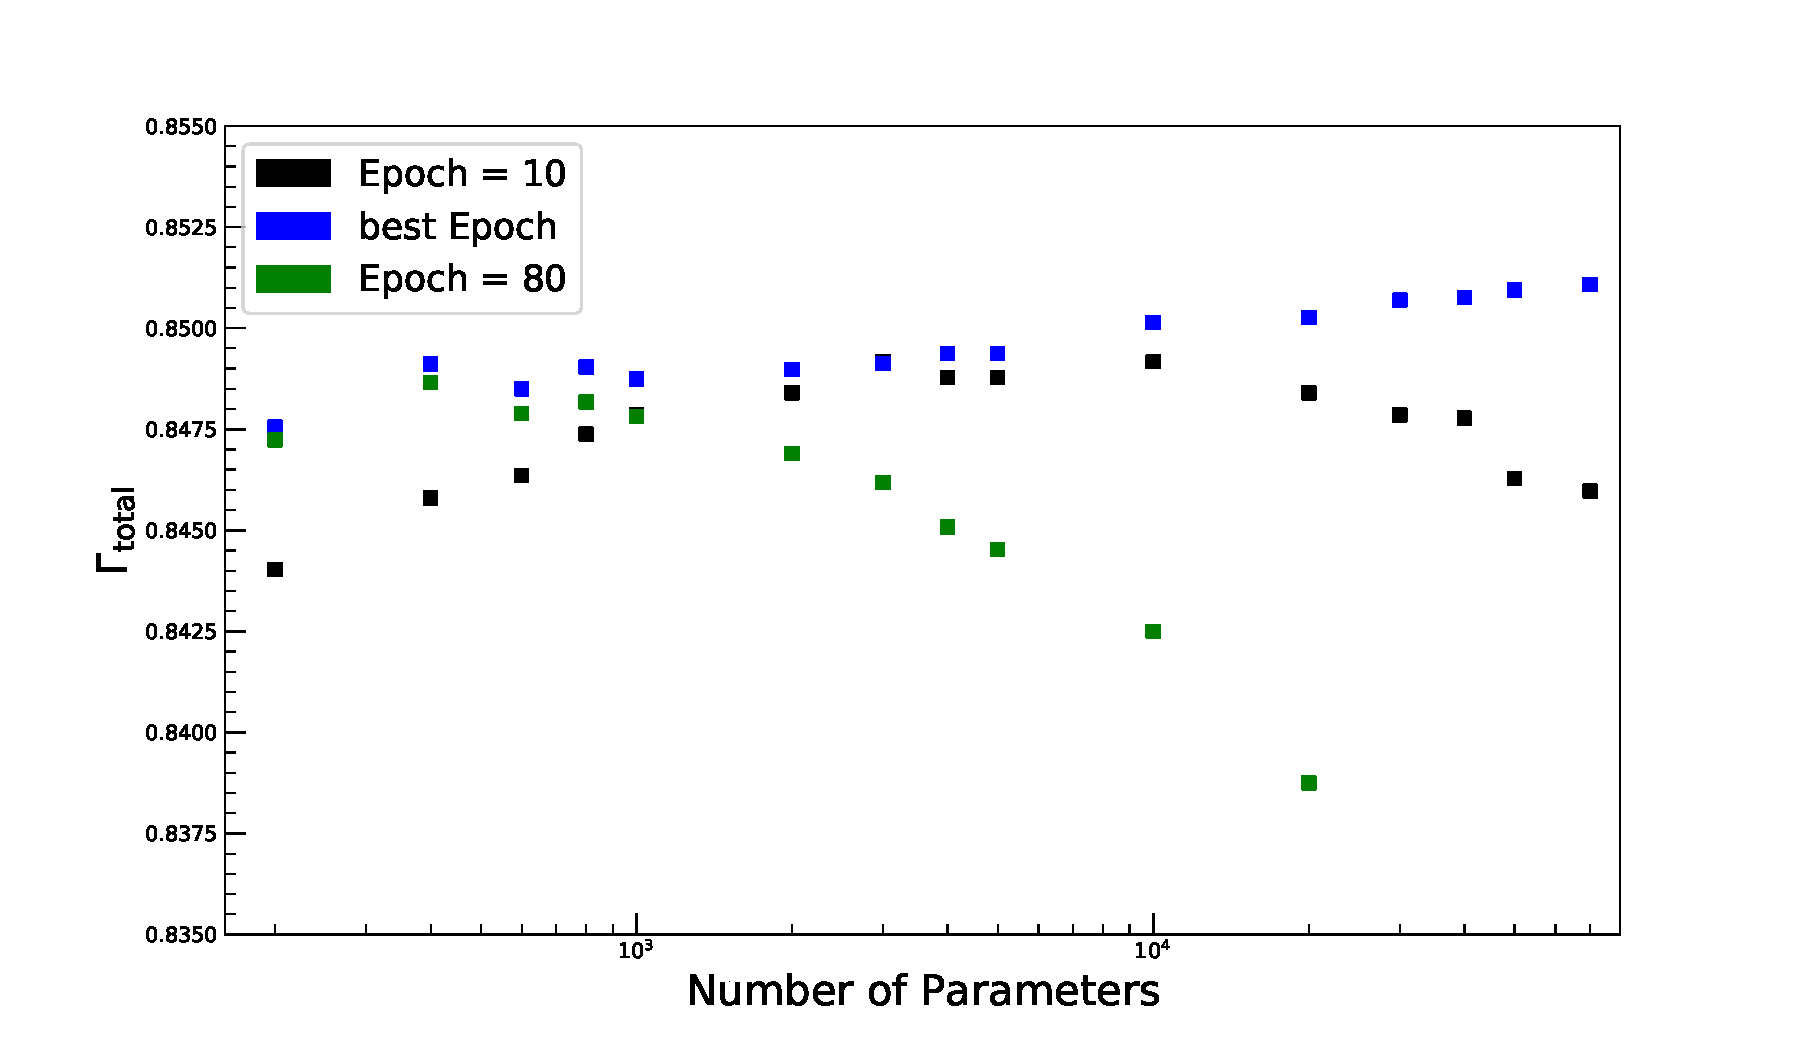
\includegraphics[width=\linewidth]{figs/FNN/AucPara_Fixed}
\caption{The averaged AUCs of FNNs with different number of parameters where the training is stopped after 10, 80 and at the best-performing Epoch. The average includes the AUCs of the 4 best-performing Neural Networks of different depth.}
\label{fig:AucPara}
\end{figure}


Figure \ref{fig:AucPara} shows the result of the search for the number of parameters where $\Gamma_{\text{total}}$ is the average of the 4 best-performing Neural Networks differing in the layer configuration. For all sizes, the standard deviation of the average is smaller than 0.001. For the blue squares, the Epoch with the highest AUC for each Neural Network was selected, whereas, for the black and green, the AUC at Epoch 10 and 80 is reported. \\
The $\Gamma_{\text{total}}$ for the best Epoch slightly increases with higher number of parameters. For Neural Networks with more than 10000 parameters, the performance gain per additional trainable parameter is minor, indicating that the current number of parameters is sufficient to obtain a reasonable separation between signal and background events. In the case of Neural Networks with few parameters, every weight needs to be fine-tuned so as to obtain the best possible performance, which can take several Epochs. On the other hand, for Neural Networks with many parameters, not all information available to a neuron is important. The learning process to identify which of the available information is key to obtain a good training result can also take several iterations. These behaviors are reflected in the distribution of the training results evaluated at Epoch 10 which show AUCs close to the best observed AUC only for Neural Networks of intermediate size.
The Neural Networks evaluated at Epoch 80 show a strong decrease in the $\Gamma_{\text{total}}$ (obtained on the test sets) with the number of parameters, indicating overtraining. The tendency of large Neural Networks to have high overtraining is especially apparent in Figure \ref{fig:OvPara} for high Epochs. However, when the AUC is calculated at the optimal Epoch, this dependency is significantly attenuated. \\

\begin{figure}[H]
\centering
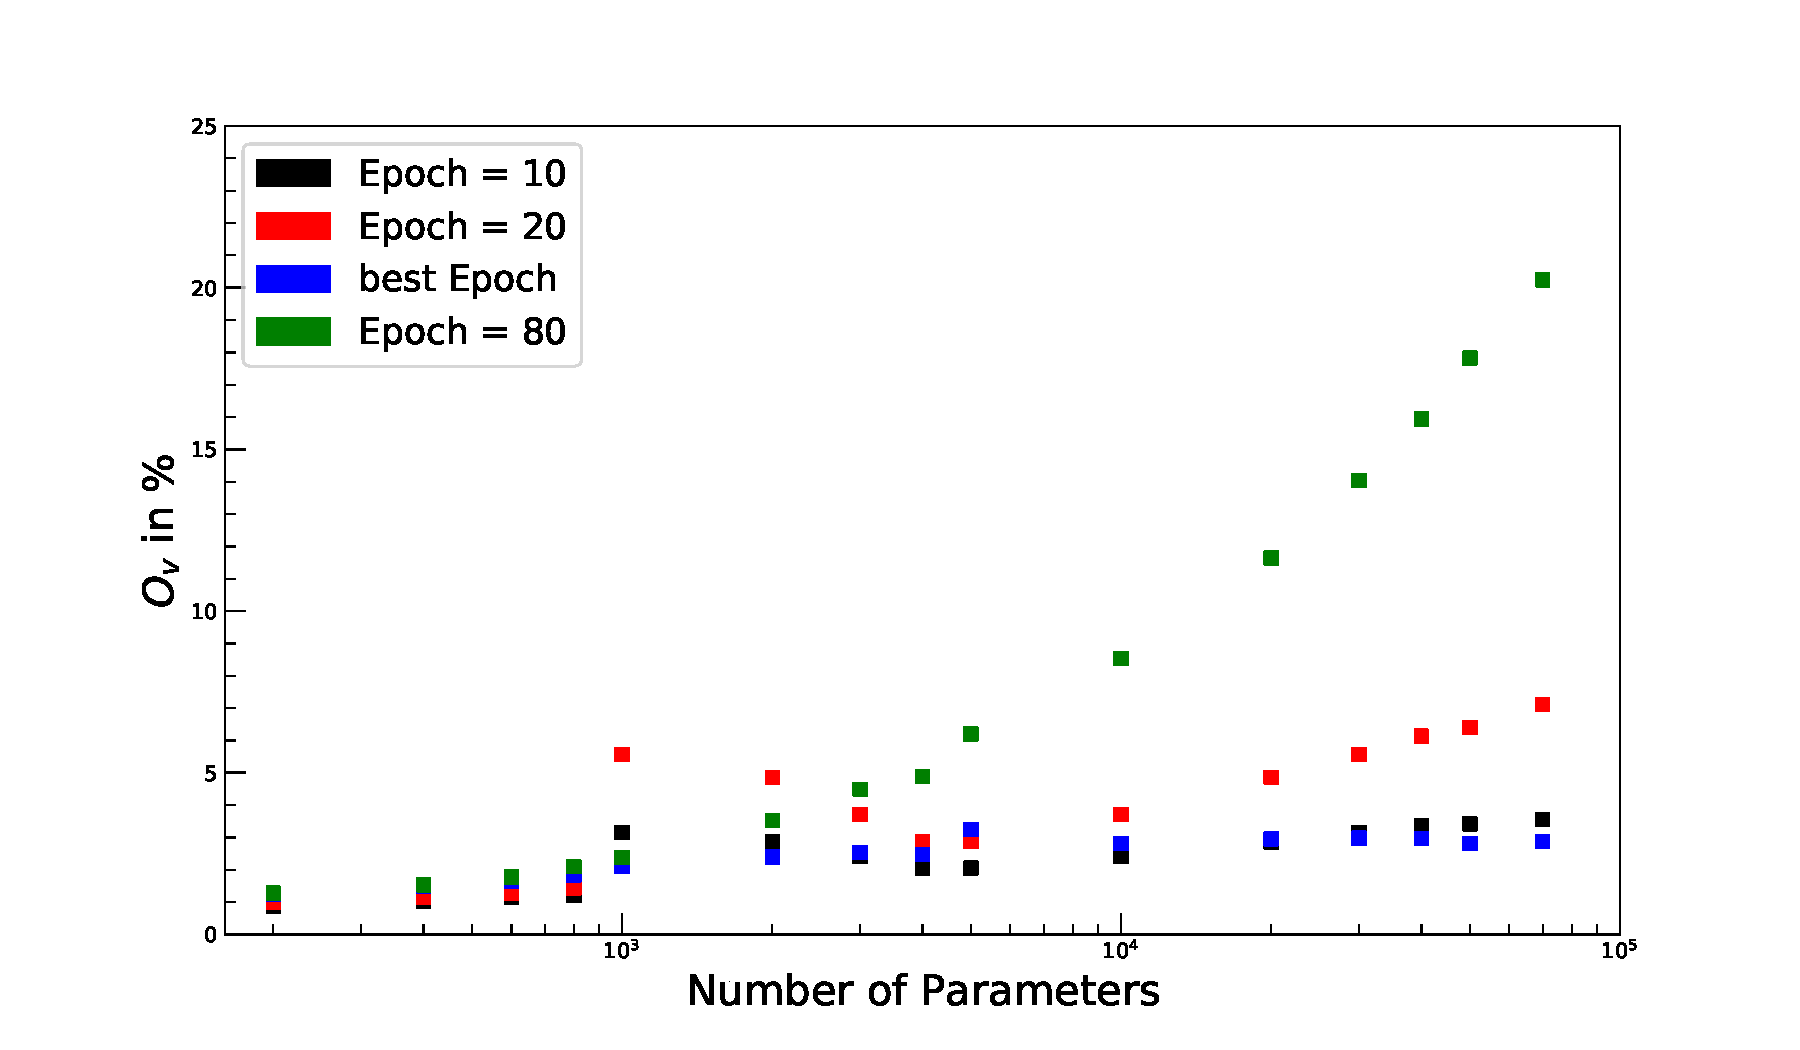
\includegraphics[width=\linewidth]{figs/FNN/OvPara_Fixed}
\caption{The average overtraining for different FNN configurations. The training is stopped after 10, 20, 80 and at the best-performing Epoch. The average includes the overtrainings of the 4 best-performing Neural Networks of different depth.}
\label{fig:OvPara}
\end{figure}

\begin{figure}[H]
\centering
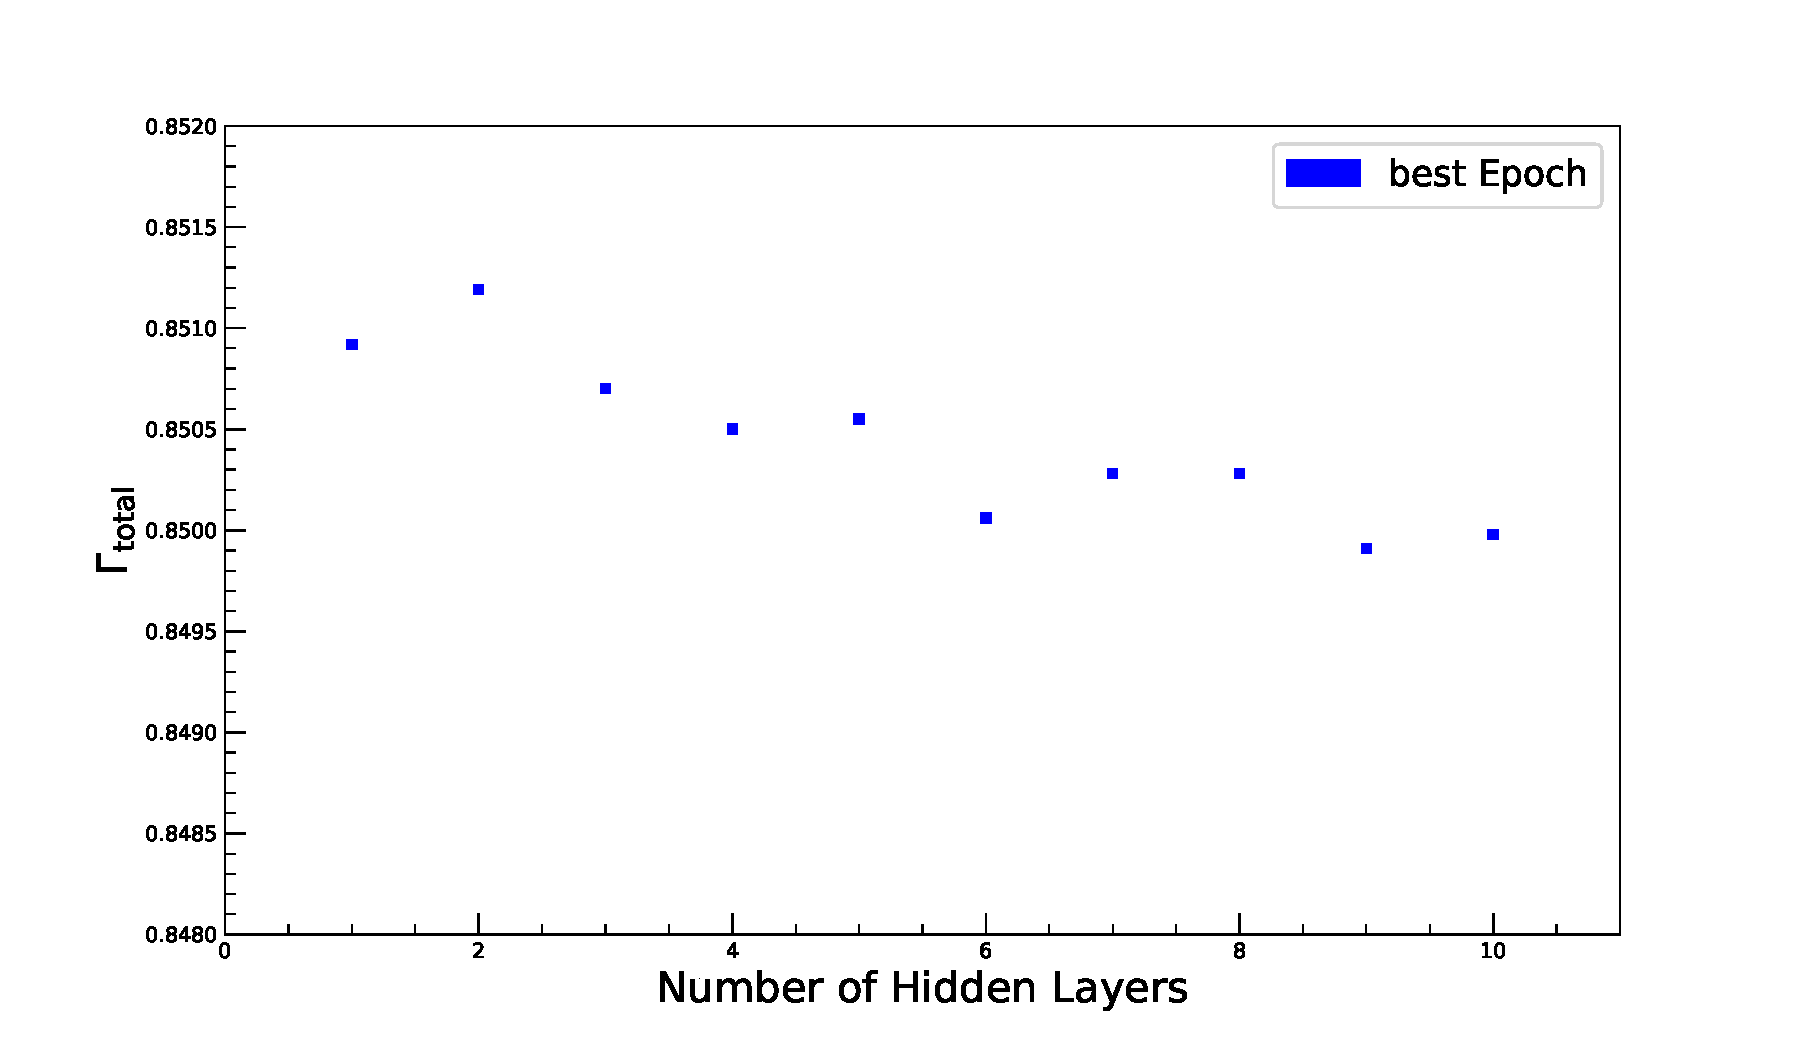
\includegraphics[width=\linewidth]{figs/FNN/Aver_LayersAuc}
\caption{The average AUC for FNNs with different numbers of hidden layers. The average includes the AUCs of the 4 best-performing Neural Networks of different size.}
\label{fig:AucLayers}
\end{figure}

\newpage

In Figure \ref{fig:AucLayers}, the average AUCs of Neural Networks with different numbers of hidden layers are shown. The average includes the 4 best-performing Neural Networks of different size. The FNNs showing the highest AUC are models with low numbers of hidden layers, especially those with two layers. The overtraining was observed to be independent of the number of hidden layers. \\
The overall performance gained by varying the number of parameters and layers is small compared to the performance gained by hyperparameter tuning. This is because the selected optimization algorithm Adam is very stable in its final performance, in combination with a reasonable initial learning rate. A cross-check using mini-batch Stochastic Gradient Descent (SGD) showed that, for this algorithm, the performance does depend more on the number of parameters. \\
Summarizing the obtained results, it can be stated that a Neural Network for hyperparameter tuning should have more than 10000 parameters to ensure high flexibility and less than 30000 to avoid high overtraining.
For the studies on learning rate, activation function, and weight initialization, a Neural Network with 20000 parameters and 2 hidden layers is selected. Its overtraining is shown in Figure \ref{fig:RegionPara} together with the overtraining of other Neural Networks in the region of interest.


\begin{figure}[H]
\centering
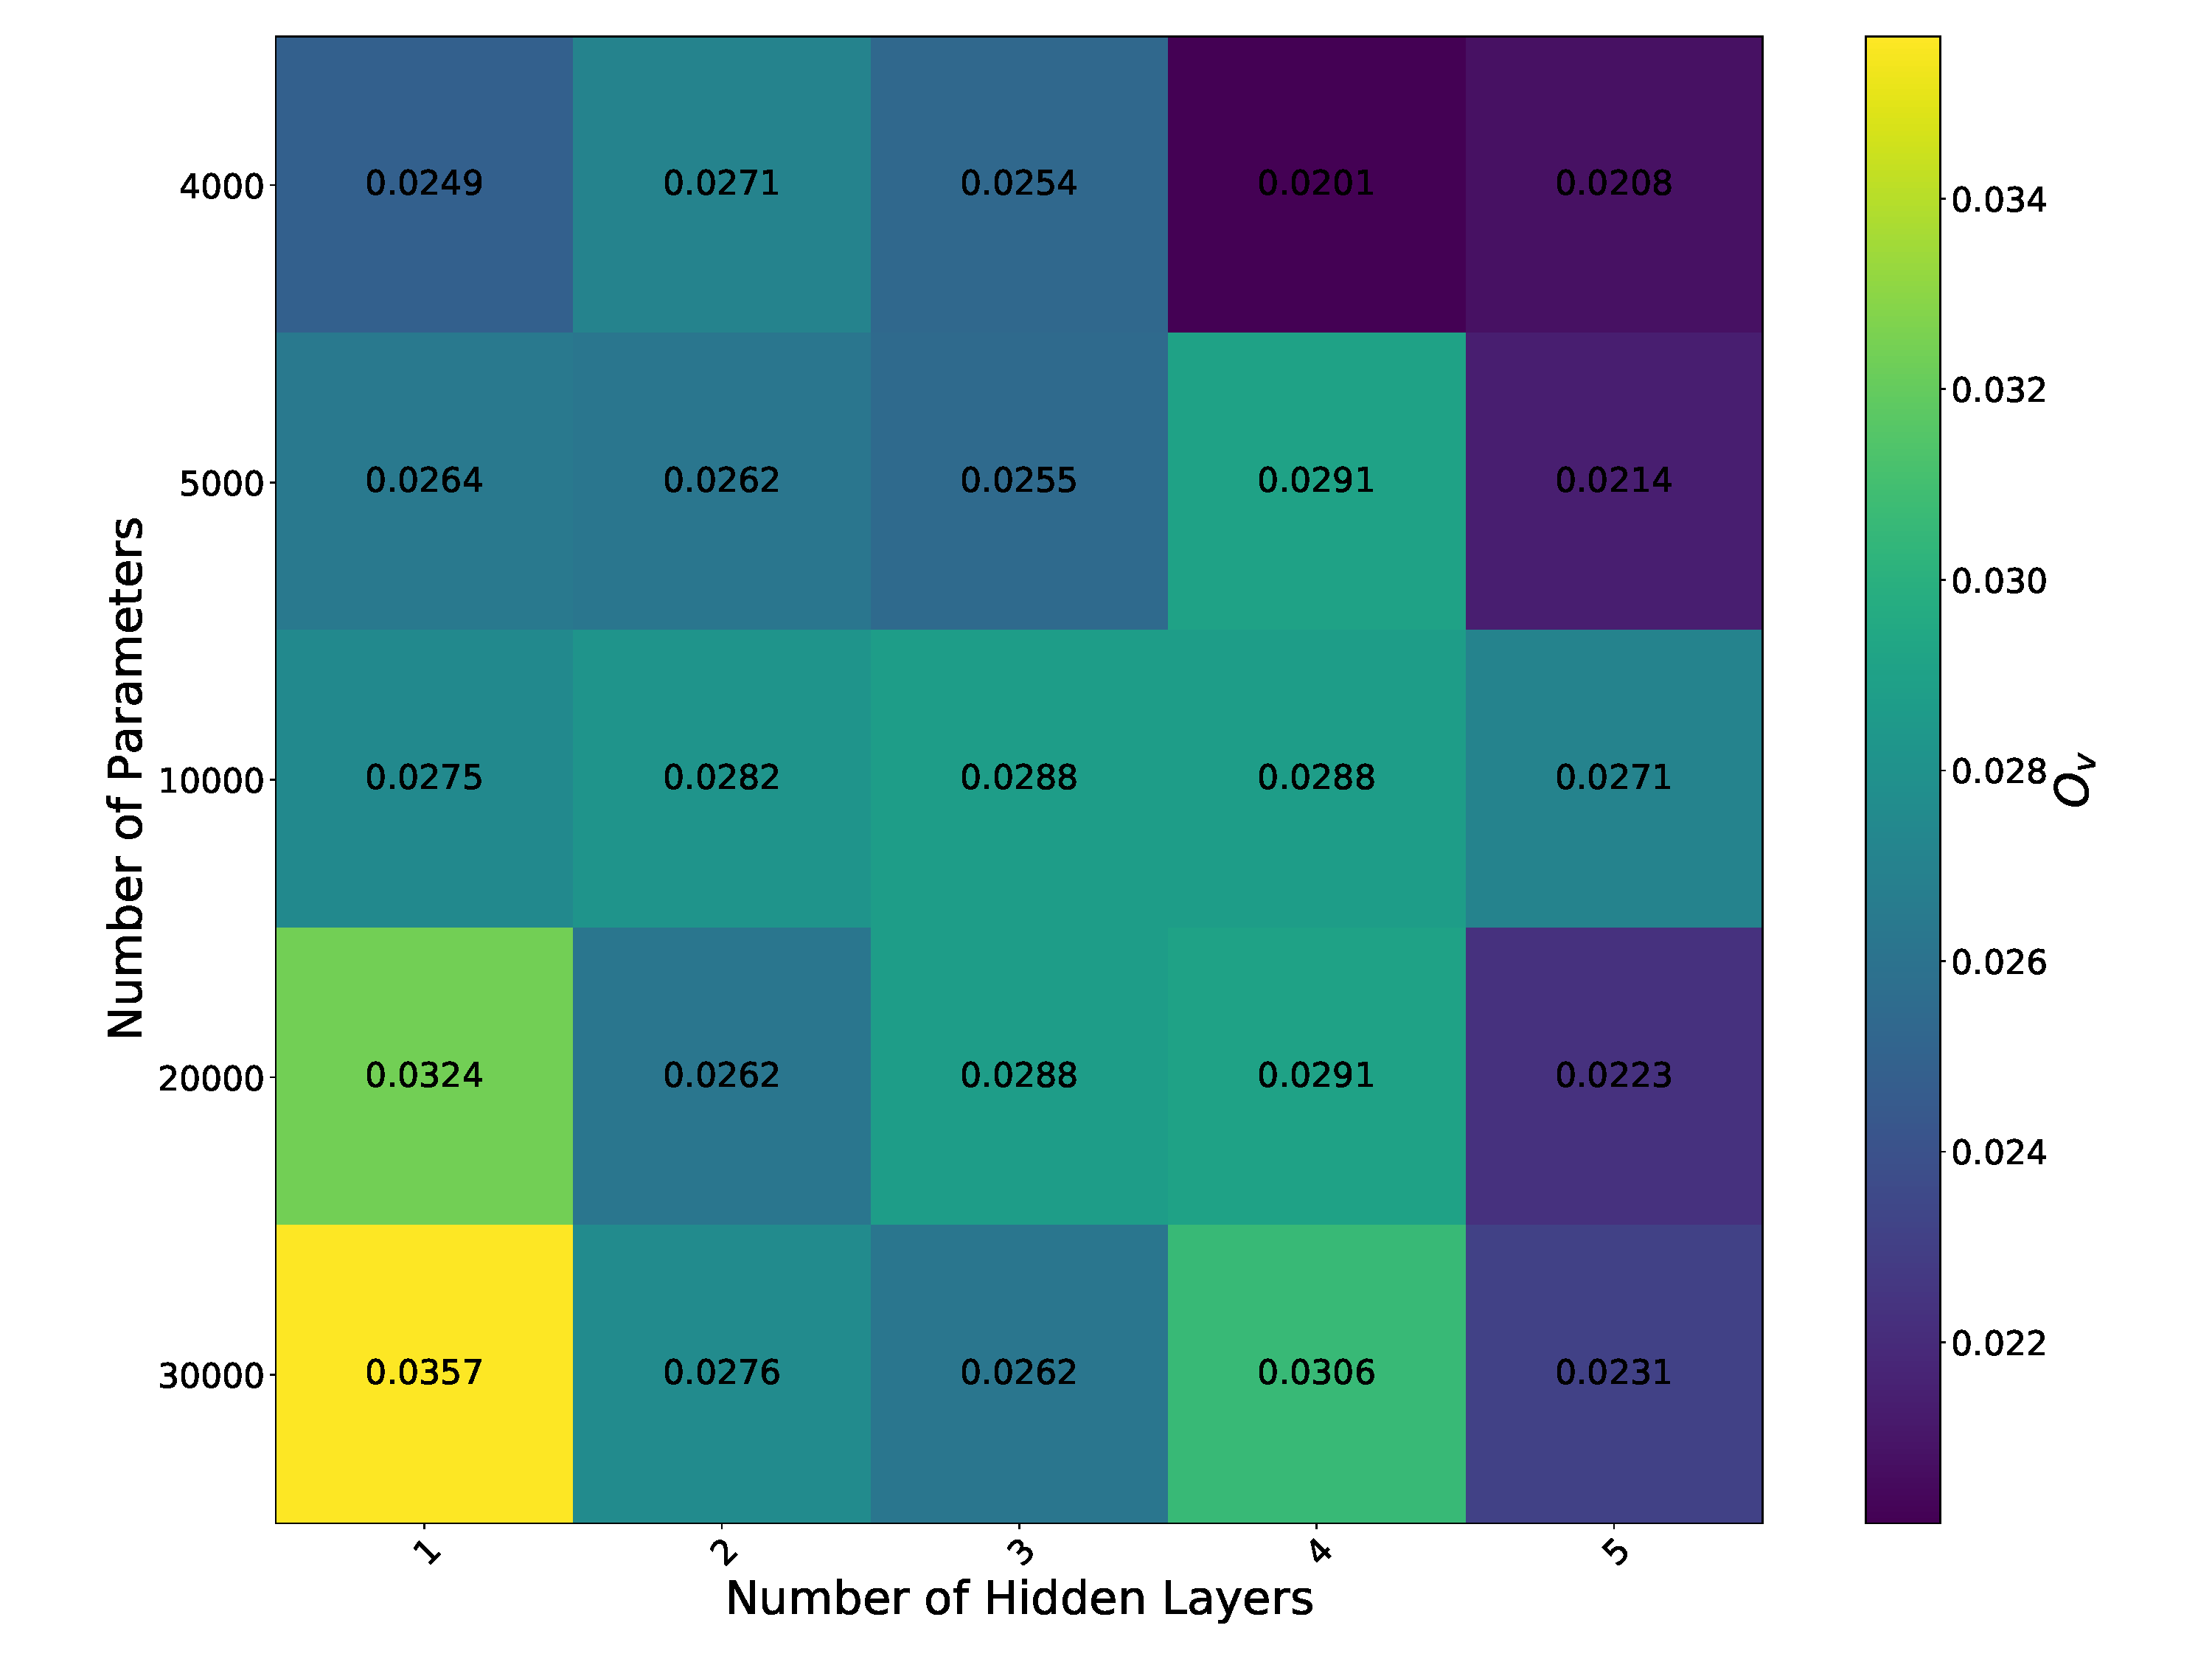
\includegraphics[width=\linewidth]{figs/FNN/Heat_ParaLayers}
\caption{The overtraining for FNNs of different sizes and depth, in the region where the observed AUCs are close to the best-performance obtained.}
\label{fig:RegionPara}
\end{figure}

\newpage

\paragraph{Weight Initialization and Activation Functions} \mbox{} \\

The Neural Networks architecture selected in the last sub-section is now selected to study the influence of activation functions and weight initialization on the AUC. As discussed in Section \ref{sec:optimization}, different weight initializations are designed to prevent the output of the activation functions from vanishing or exploding during the forward pass. Therefore, a high correlation between the two can be expected. \\
The effect of activation functions is studied by setting the activation function of all neurons in all hidden layers to either ReLU, leaky ReLU ($\alpha \in [0.1,0.3,0.5]$), ELU ($\alpha = 1$), or  SELU. For each activation function, different weight initializations namely Glorot, He, and Lecun with normal and uniform distributions are tested. The activation function of the output layer remains to be the Sigmoid function. The biases are initialized to zero. All other parameters are kept constant. \\

\begin{figure}[H]
\centering
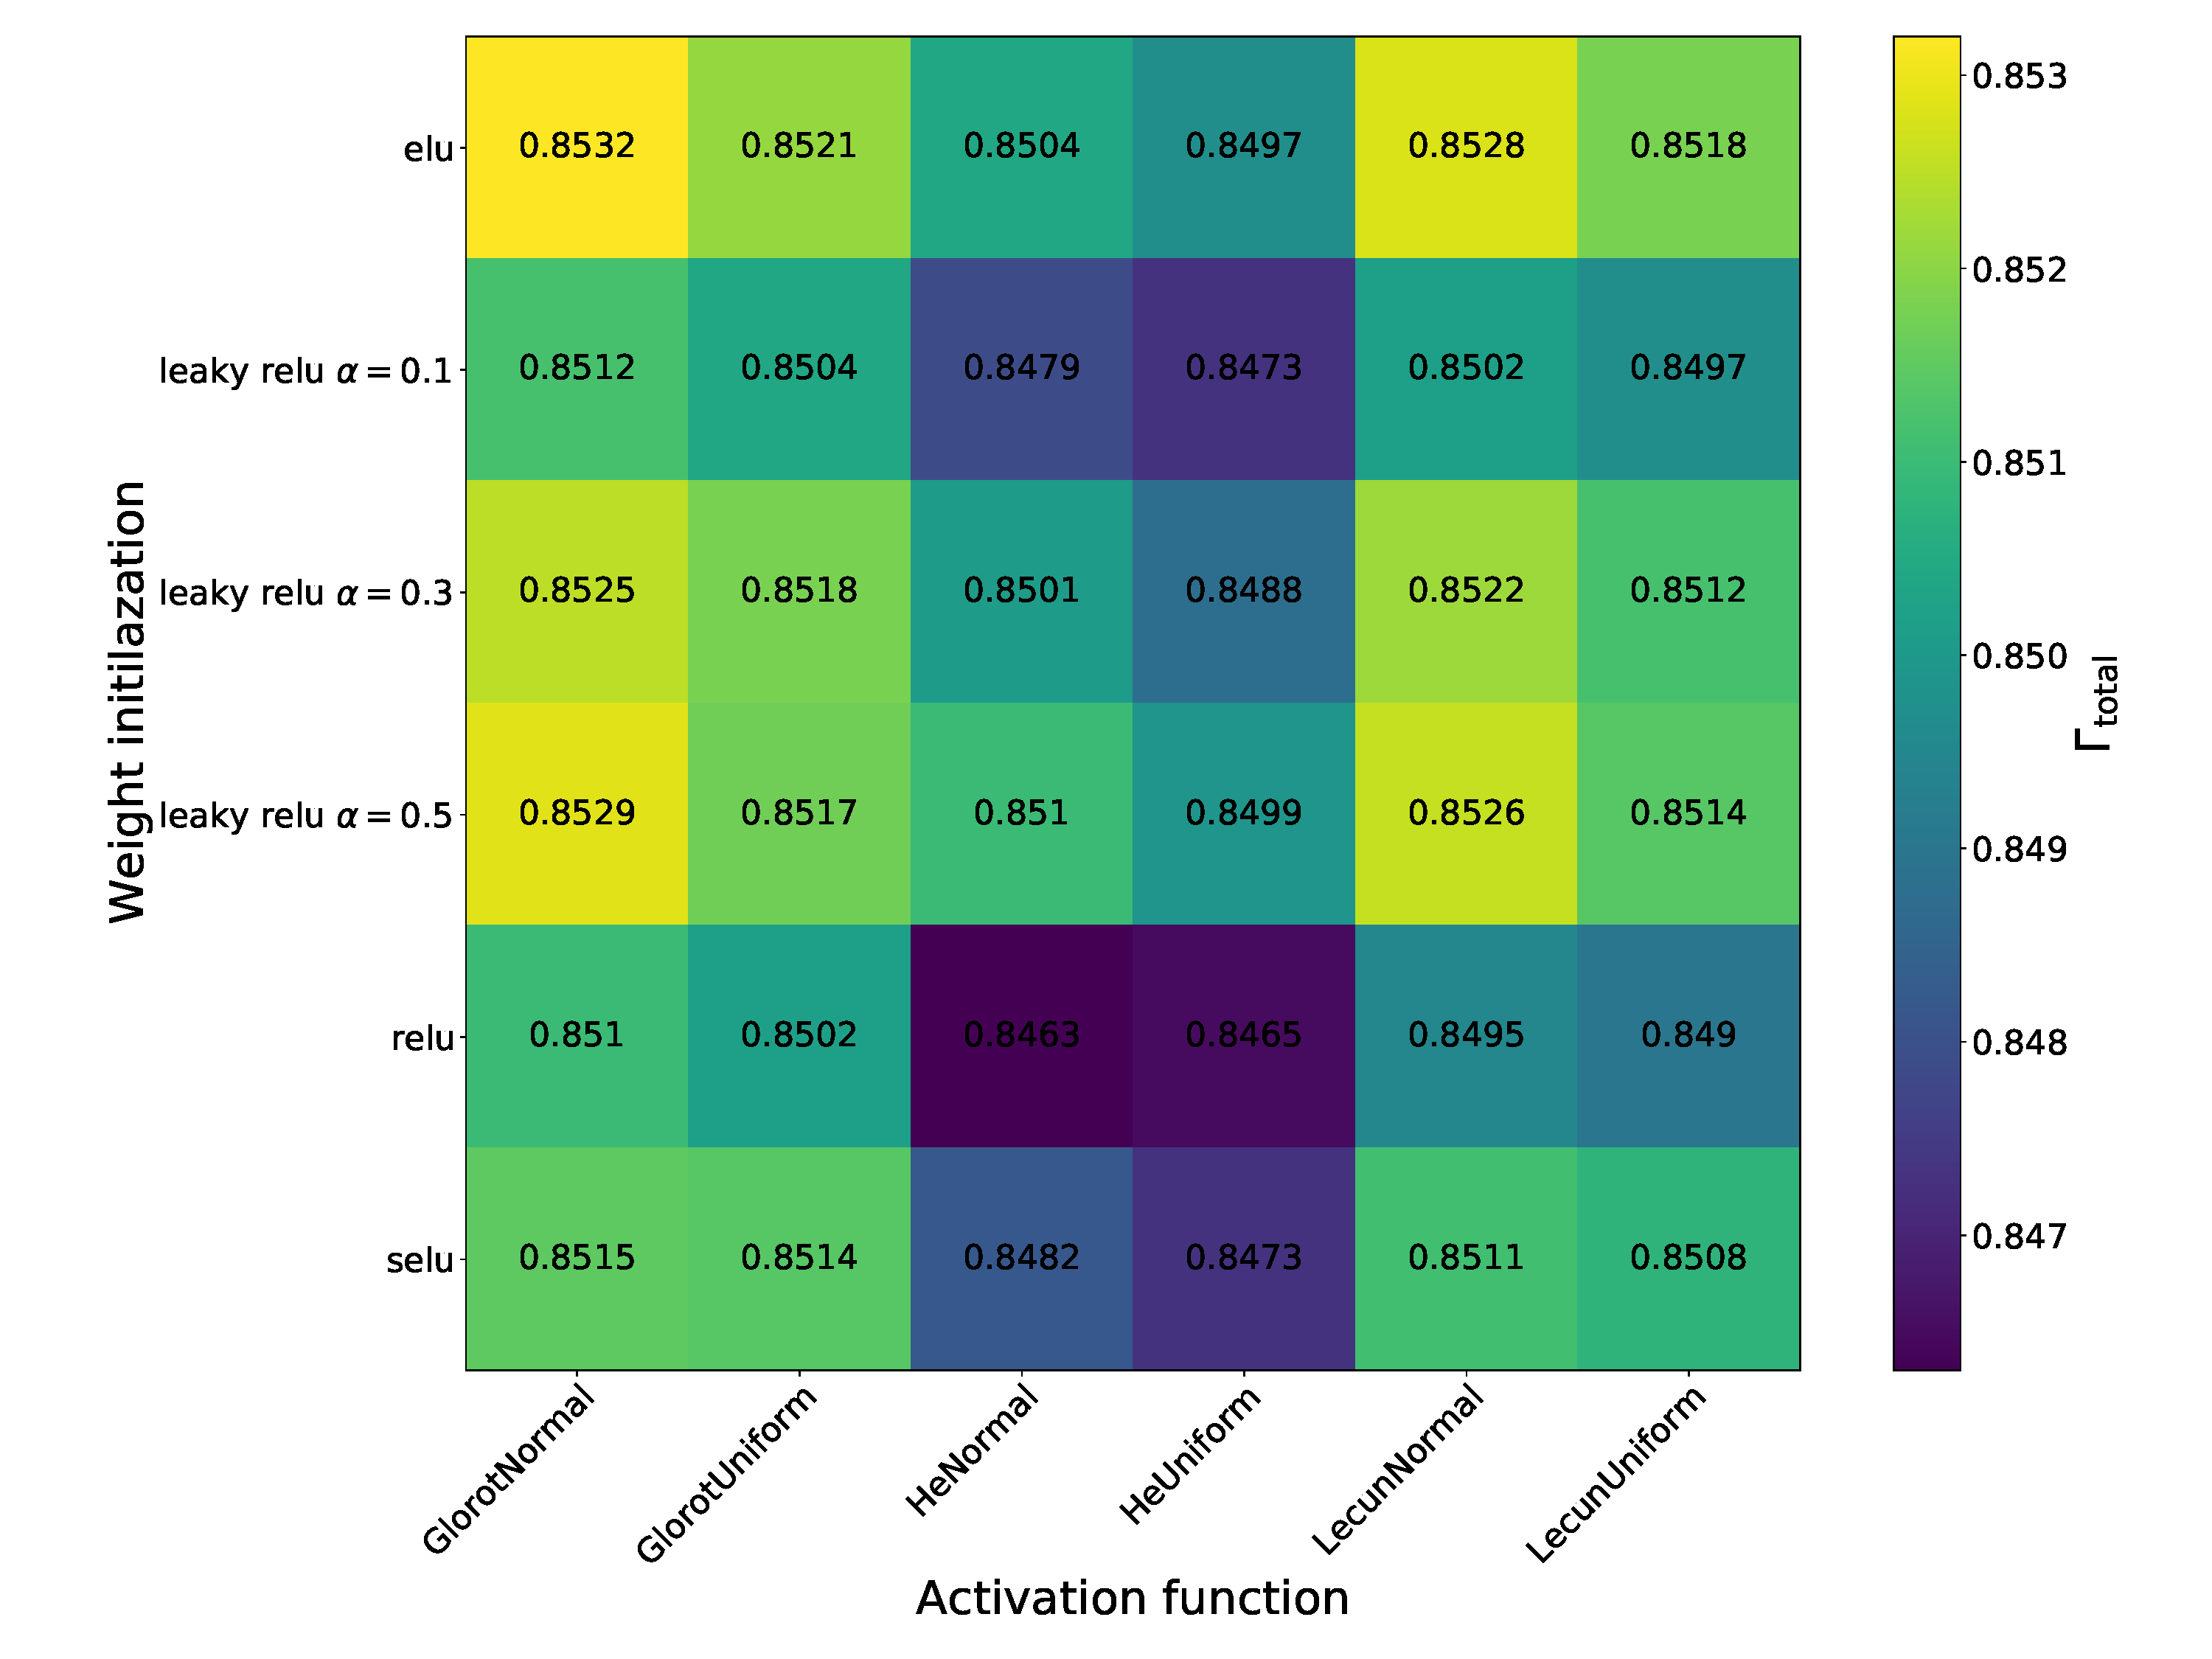
\includegraphics[width=\linewidth]{figs/FNN/Heat_Activ}
\caption{AUCs obtained for different choices of activation functions and weight initialization.}
\label{fig:HeatActiv}
\end{figure}

Figure \ref{fig:HeatActiv} shows the obtained AUCs for all combinations while Figure \ref{fig:OvActiv} shows the corresponding overtraining values. The best performance is reached when ELU is combined with the Glorot normal distribution weight initialization, which is the weight initialization that works best for all considered activation functions. The difference between normally and uniformly distributed weight initializations is minor but normally distributed initializations result in slightly higher AUC. \\
The ReLU activation function is outperformed for all considered by all other activation functions. This indicating that a training in which some weights are not updated, as is the case for ReLU, is not beneficial for this application. In fact, the performance increases with the slope constant $\alpha$ for leaky ReLU. In the case of ELU, a smooth transition between the output values for negative and positive net input results in the best $\Gamma_{\text{total}}$ for all weight initializations. The SELU activation function, specifically designed for FNNs, does not lead to an improved result compared to ELU. \\
The overtraining for all considered activation functions and weight initializations remains below 5\%. Counter-intuitively, the Neural Networks with the highest AUC also have the smallest overtraining and the lowest $\Gamma_{\text{total}}$ on the training dataset. Therefore, the additional performance gains come from the reduction of overtraining by the activation functions and weight initializations.

\begin{figure}[H]
\centering
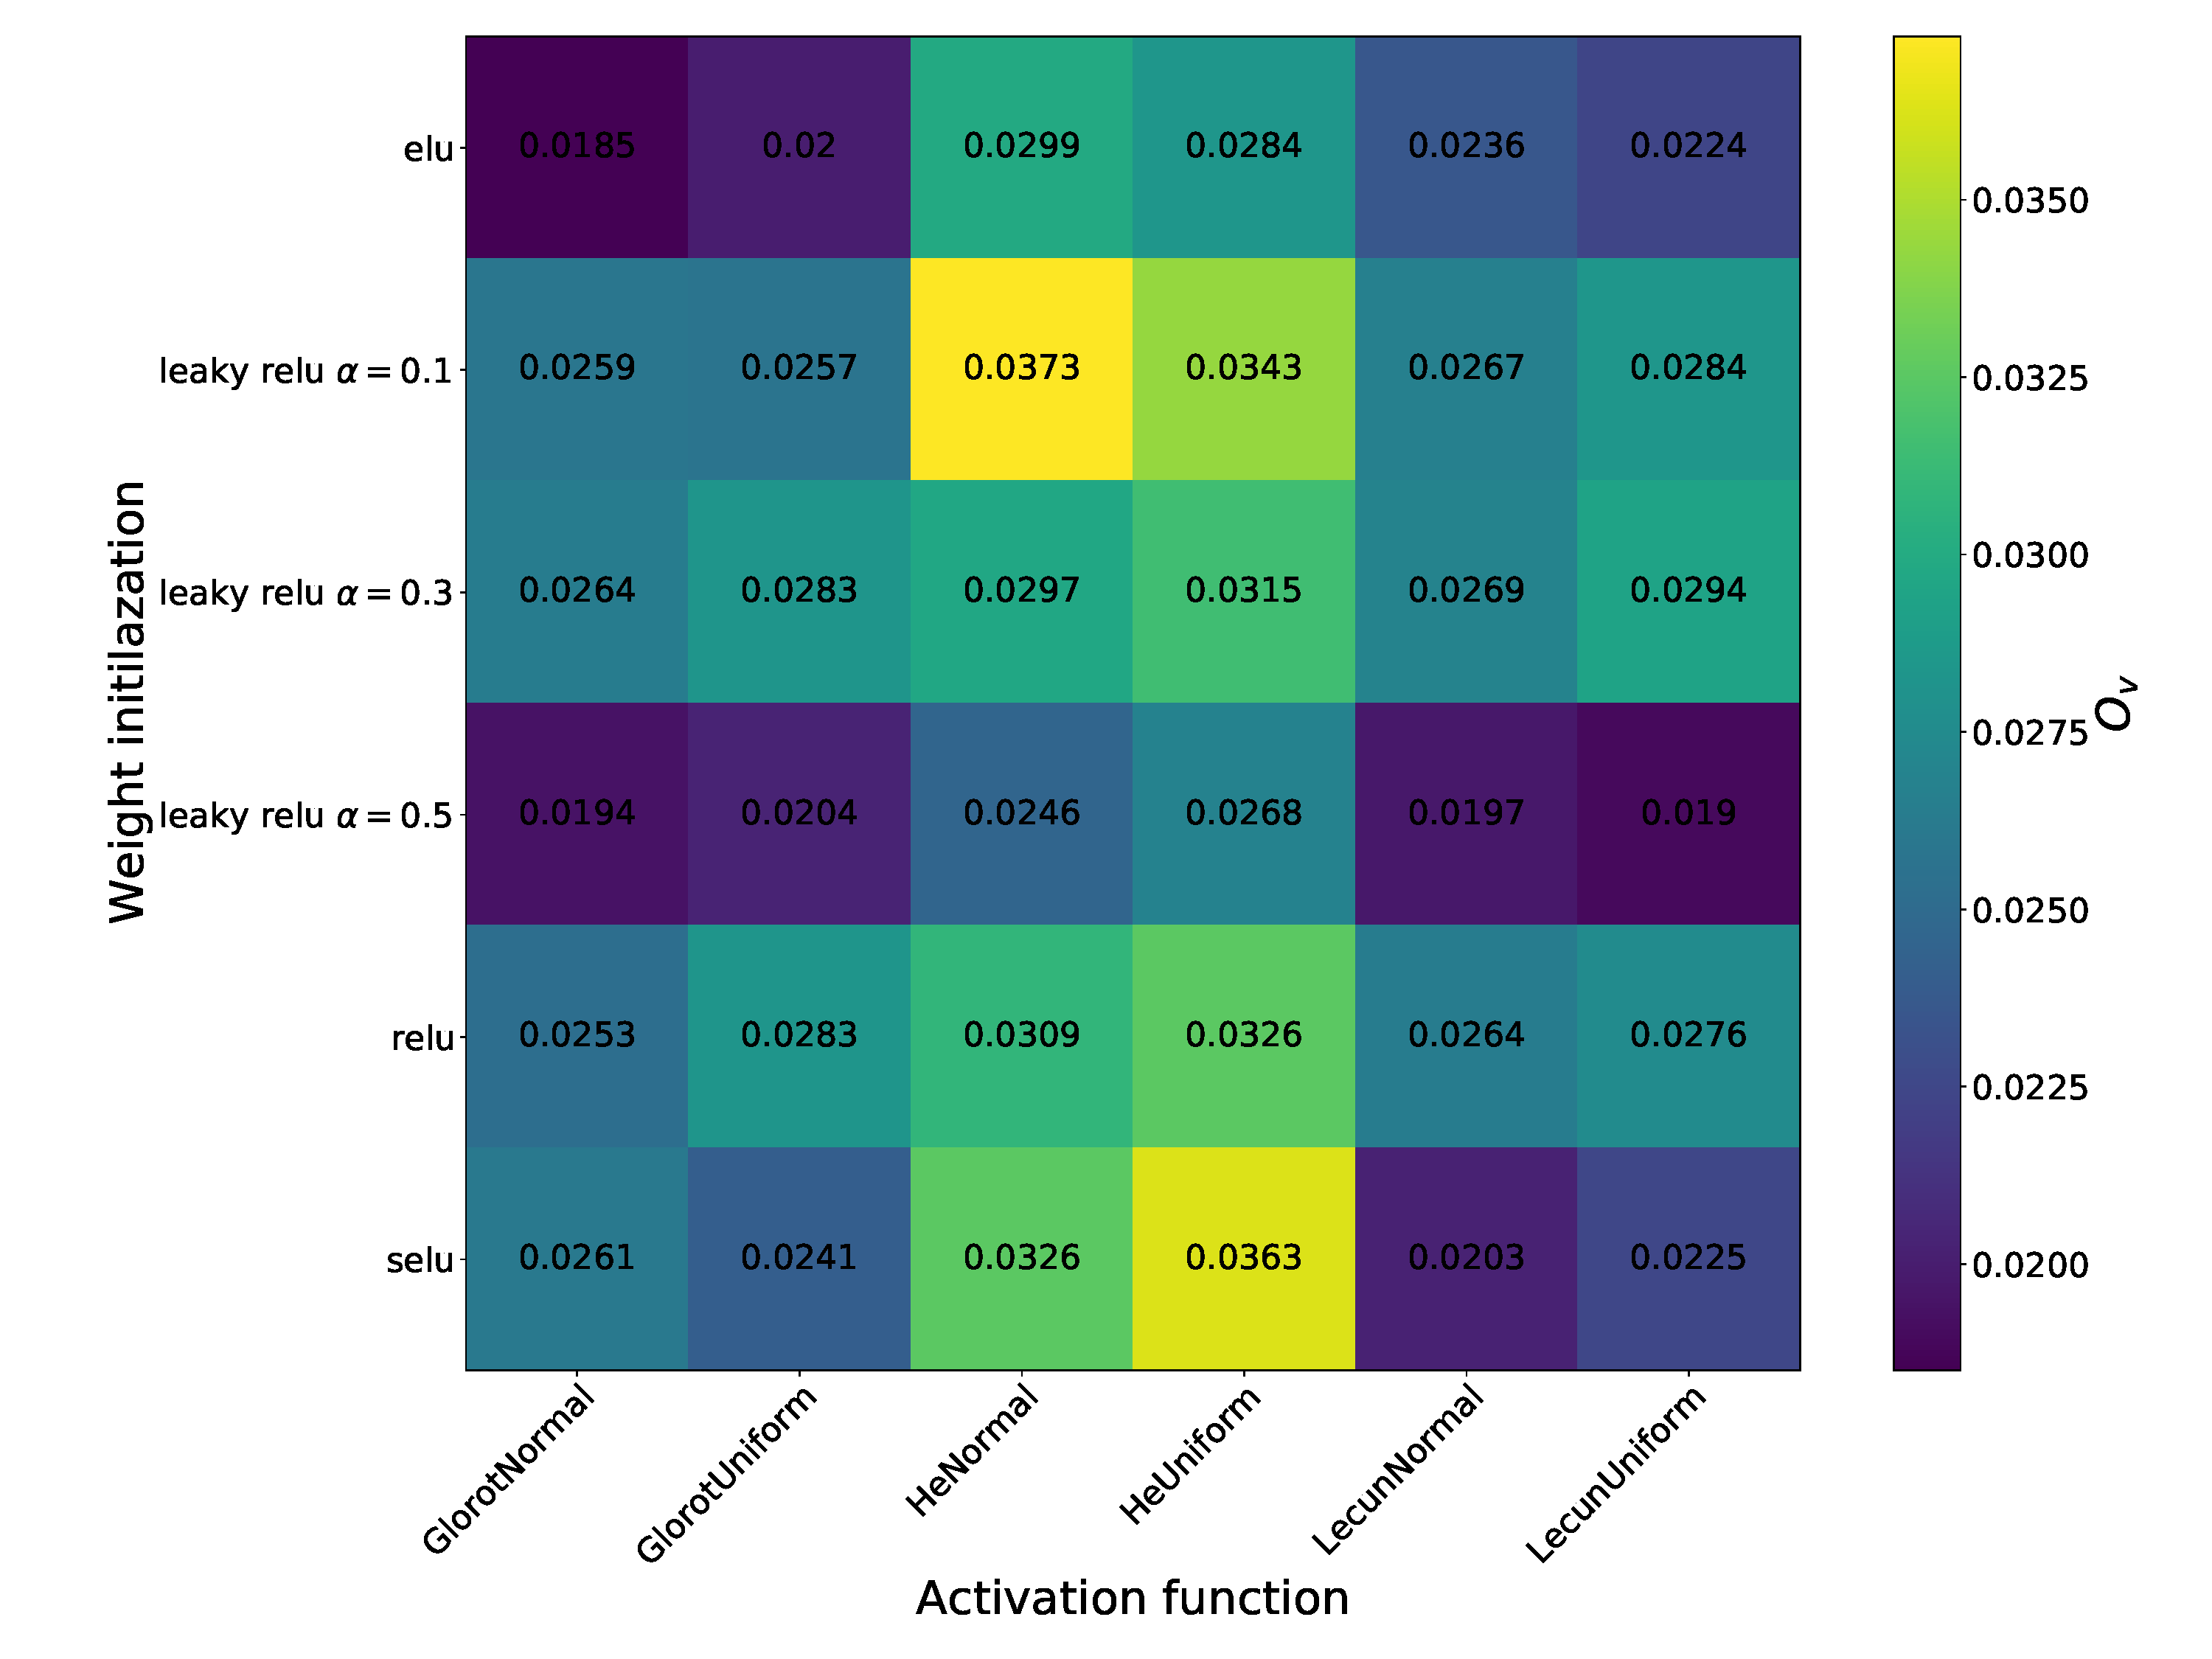
\includegraphics[width=\linewidth]{figs/FNN/Heat_Ovactiv}
\caption{The overtraining for different choices of activation functions and weight initialization.}
\label{fig:OvActiv}
\end{figure}

\newpage

\paragraph{Learning Rate and Optimization Algorithms}  \mbox{} \\

Building upon the results obtained in the first two studies, the performance for different optimization algorithms is investigated. The most impactful hyperparameters of the optimization algorithm are the learning rate, determining the step size of every weight update, and the batch size which is the number of events used during one iteration of the training. \\
Three different optimization algorithms are considered in this thesis: SGD, Adam, and Rmsprop. For each optimization algorithm, distinct learning rates are investigated together with varying the batch size. The different batch sizes are selected as powers of 2 and range from $2^8 = 256$ to $2^{14} = 16384$. All other ingredients of the Neural Network are kept constant. \\


\begin{figure}[H]
\centering
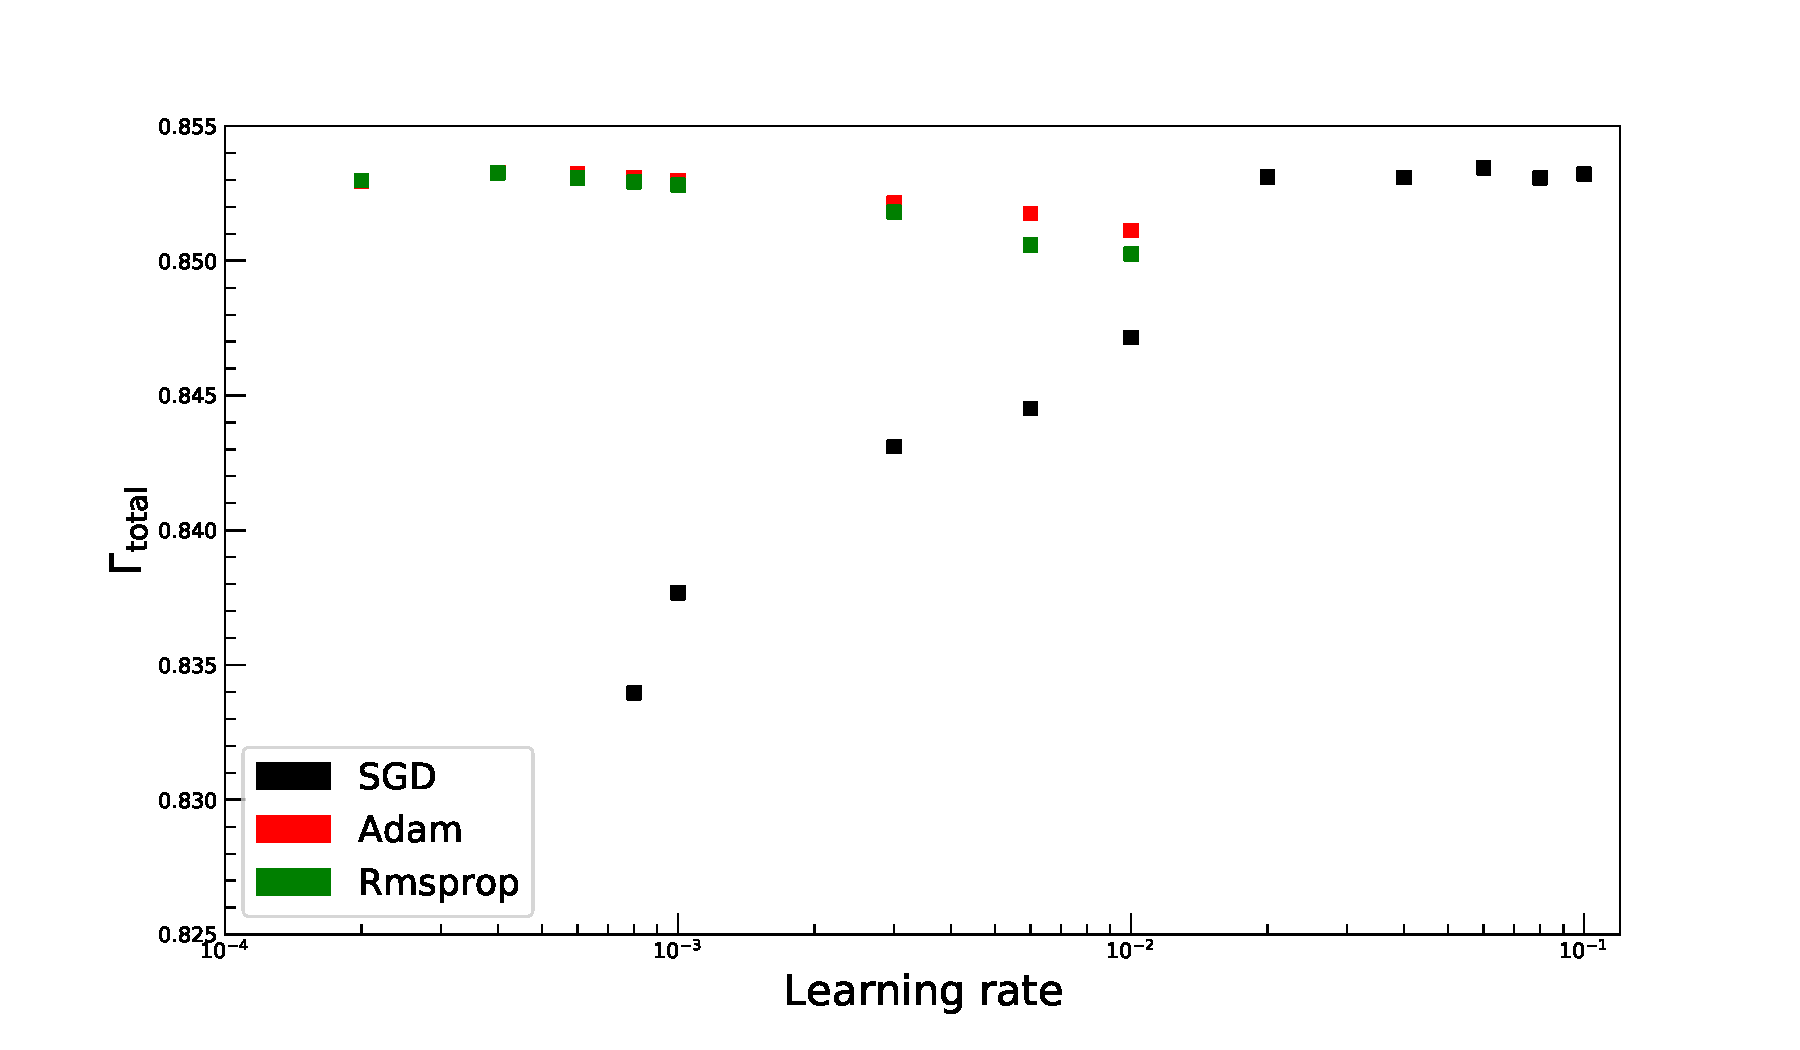
\includegraphics[width=\linewidth]{figs/FNN/LrAuc_All}
\caption{The obtained average AUC of FNNs with different learning rates and three distinct optimization algorithms.  The average includes the AUCs of the 3 best-performing Neural Networks with different batch sizes.}
\label{fig:LrAuc}
\end{figure}

Figure \ref{fig:LrAuc} shows the observed $\Gamma_{\text{total}}$ values for different learning rates and optimization algorithms while averaging over the 3 best-performing batch sizes for each learning rate. All three investigated optimization algorithms show a similar peak performance. The improvements gained by fine-tuning the learning rate within one order of magnitude are minor. For Adam and Rmsprop, even learning rates of one order of magnitude higher than the optimal observed learning rate result in only slightly worth AUCs while SGD is more sensitive. The reason being, Adam and Rmsprop calculate individually optimized learning rates for different parameters (weights and biases) based on the initial learning rate. On the other hand, SGD always applies the same learning rate for all parameters. This internal optimization is also reflected in the fact that Neural Networks trained with SGD tend to need more Epochs until the best AUC is reached, compared to Neural Networks trained with Rmsprop or Adam. All considered models have a similar overtraining for all considered learning rates, shown in Figure \ref{fig:OvLr}. The choice of the optimization algorithm used for training did not influence the overtraining. The Neural Networks with less than 1\% of overtraining are the models that have poor AUC, indicating that the training for these models did not converge. \\

\begin{figure}[H]
\centering
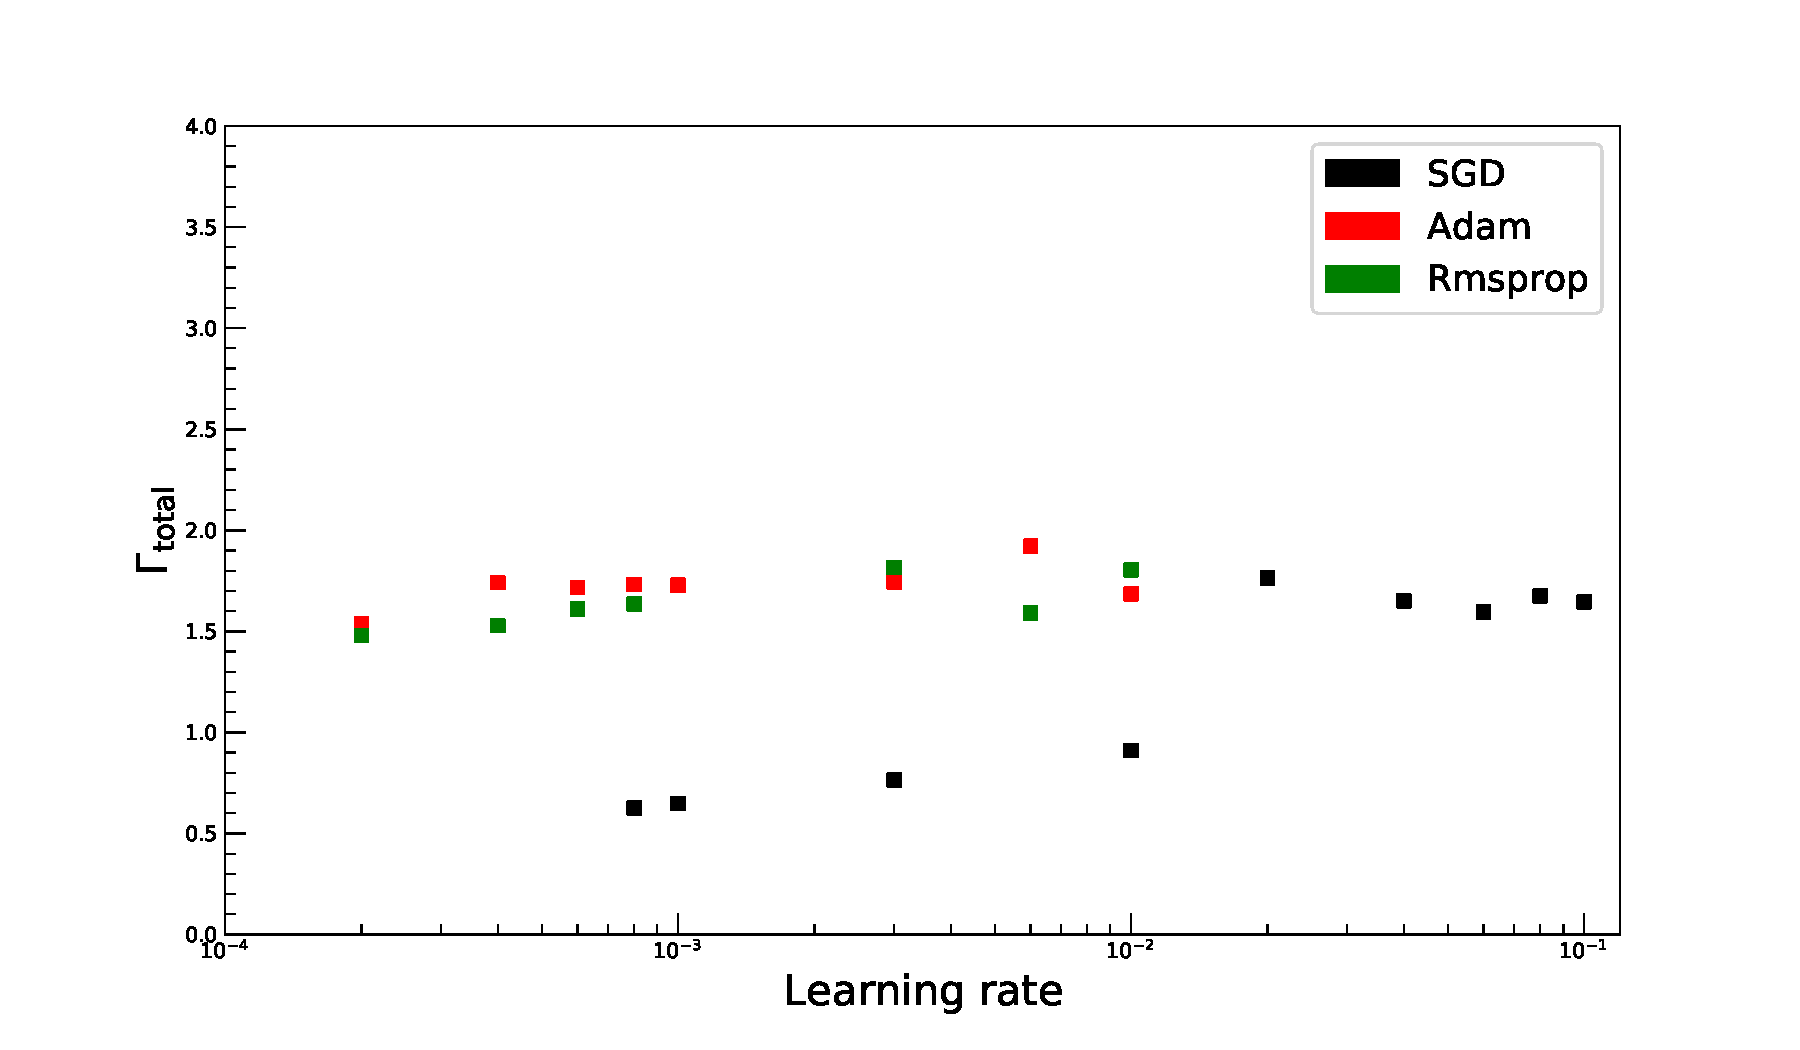
\includegraphics[width=\linewidth]{figs/FNN/LrOv_Fixed}
\caption{The overtraining of FNNs for different learning rates $Lr$ and three distinct optimization algorithms.}
\label{fig:OvLr}
\end{figure}

\begin{figure}[H]
\centering
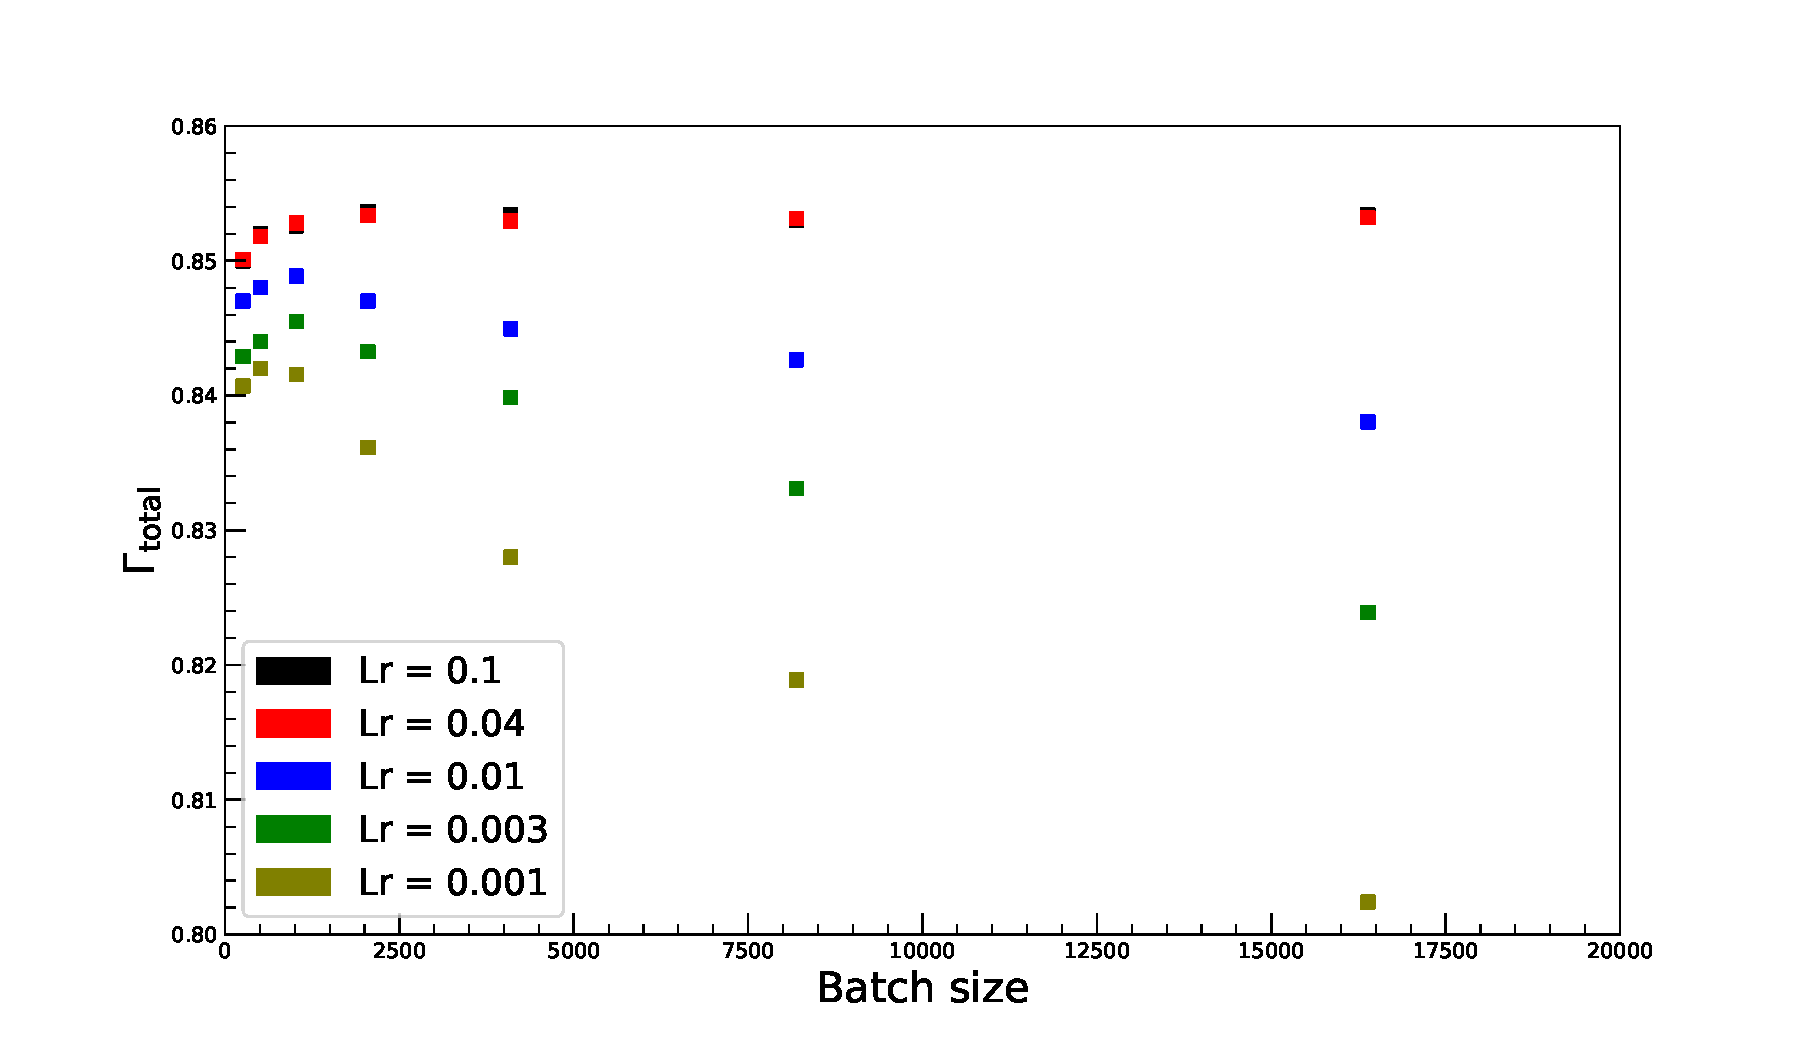
\includegraphics[width=\linewidth]{figs/FNN/BatchAuc_SGD}
\caption{The AUC as a function of the batch size and the learning rate. The Neural Networks are trained using SGD.}
\label{fig:SGDBatch}
\end{figure}

In order to study the dependence of $\Gamma_{\text{total}}$ on the batch size, Figure \ref{fig:SGDBatch} exclusively shows the results obtained by using SGD as the optimization algorithm. The AUC for learning rates close to the optimal observed choice (black and red) is almost independent of the batch size. On the other hand, for smaller learning rates, the batch size has a significant impact. This is because, for those Neural Networks the maximum considered number of 120 Epochs is reached which in turn is a direct consequence of the small batch size. Neural Networks trained with small batch sizes perform less weight updates per Epoch. When the maximum number of Epochs is not sufficiently high, the small number of weight updates leads to a non-optimal weight configuration that decreases the obtained AUC. The drop in peak performance for small batch sizes ($< 2000$) can be attributed to the fact that a small batch may not contain events from all backgrounds. The weight updates calculated based on this batch may not be accurate enough to lead to the optimal weight configuration during training. \\
The best Neural Network obtained uses Adam with a learning rate of 0.003 and a batch size of 2048.  The maximum  $\Gamma_{\text{total}}$ reached is 0.853, with an overtraining of 0.016 on the testing set.




\paragraph{Polynomial Learning Rate Decay} \mbox{} \\
 

\begin{figure}[H]
\begin{subfigure}{.33\textwidth}
  \centering
  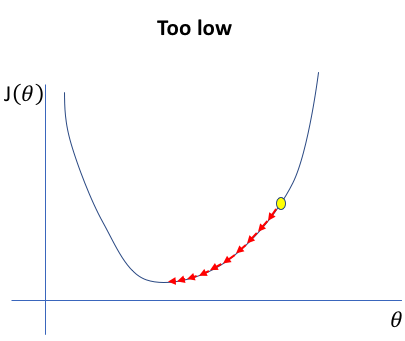
\includegraphics[width=.99\linewidth]{figs/TooLow}
  \caption{}
  \label{fig:TooLow}
\end{subfigure}%
\begin{subfigure}{.33\textwidth}
  \centering
  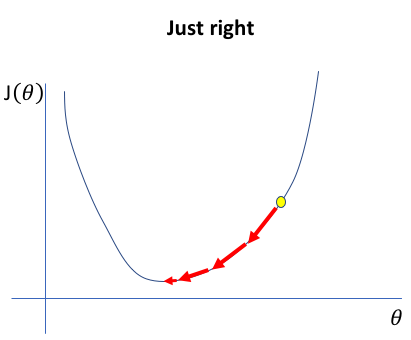
\includegraphics[width=.99\linewidth]{figs/JustRight}
  \caption{}
  \label{fig:JustRight}
\end{subfigure}
\begin{subfigure}{.33\textwidth}
  \centering
  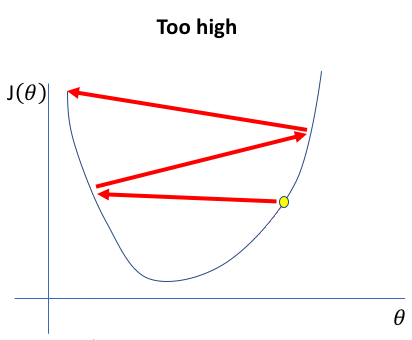
\includegraphics[width=.99\linewidth]{figs/TooHigh}
  \caption{}
  \label{fig:TooHigh}
\end{subfigure}%
\caption{Training of a Neural Network trained with a too low (a), a too high and a polynomial decaying learning rate. \cite{lrdecay} }
\label{fig:PolyTrain}
\end{figure}


Three different trainings scenarios for the same problem are shown in Figure \ref{fig:PolyTrain}. In the first case (\ref{fig:TooLow}), the learning rate is too low to reach the minimum of the Loss functions $J(\theta)$ during the training. On the other hand, if the learning rate is too large (\ref{fig:TooHigh}), the weight updates overshoot the point of best performance, resulting in a decreased AUC. Both cases can be avoided when using polynomial learning rate decay (\ref{fig:JustRight}). In polynomial learning rate decay, the initial learning rate $Lr_{\text{int}}$ is adjusted for each Epoch according to
\begin{equation}
Lr(E) = Lr_{\text{int}} \cdot (1-\frac{E}{E_{\text{tot}}})^{n}
\end{equation}
where $Lr(E)$ is the learning rate at Epoch $E$, and $n$ is the used polynomial power. For this technique, the total number of Epochs $E_{\text{total}}$ has to be fixed. Using polynomial learning rate decay results in a more smooth coverage of the training towards the minimum. \\
For the studies on polynomial learning rate decay in this thesis, SGD was selected as the optimization algorithm to investigate the gained improvements independently of the parameter-by-parameter optimization used by Adam and Rmsprop. The initial learning is varied between 0.02 and 0.3, building upon the knowledge gained in the previous sub-section. Considered polynomials have the power of 1 to 3. The other parameters of the Neural Network are kept constant. \\

\begin{figure}[H]
\centering
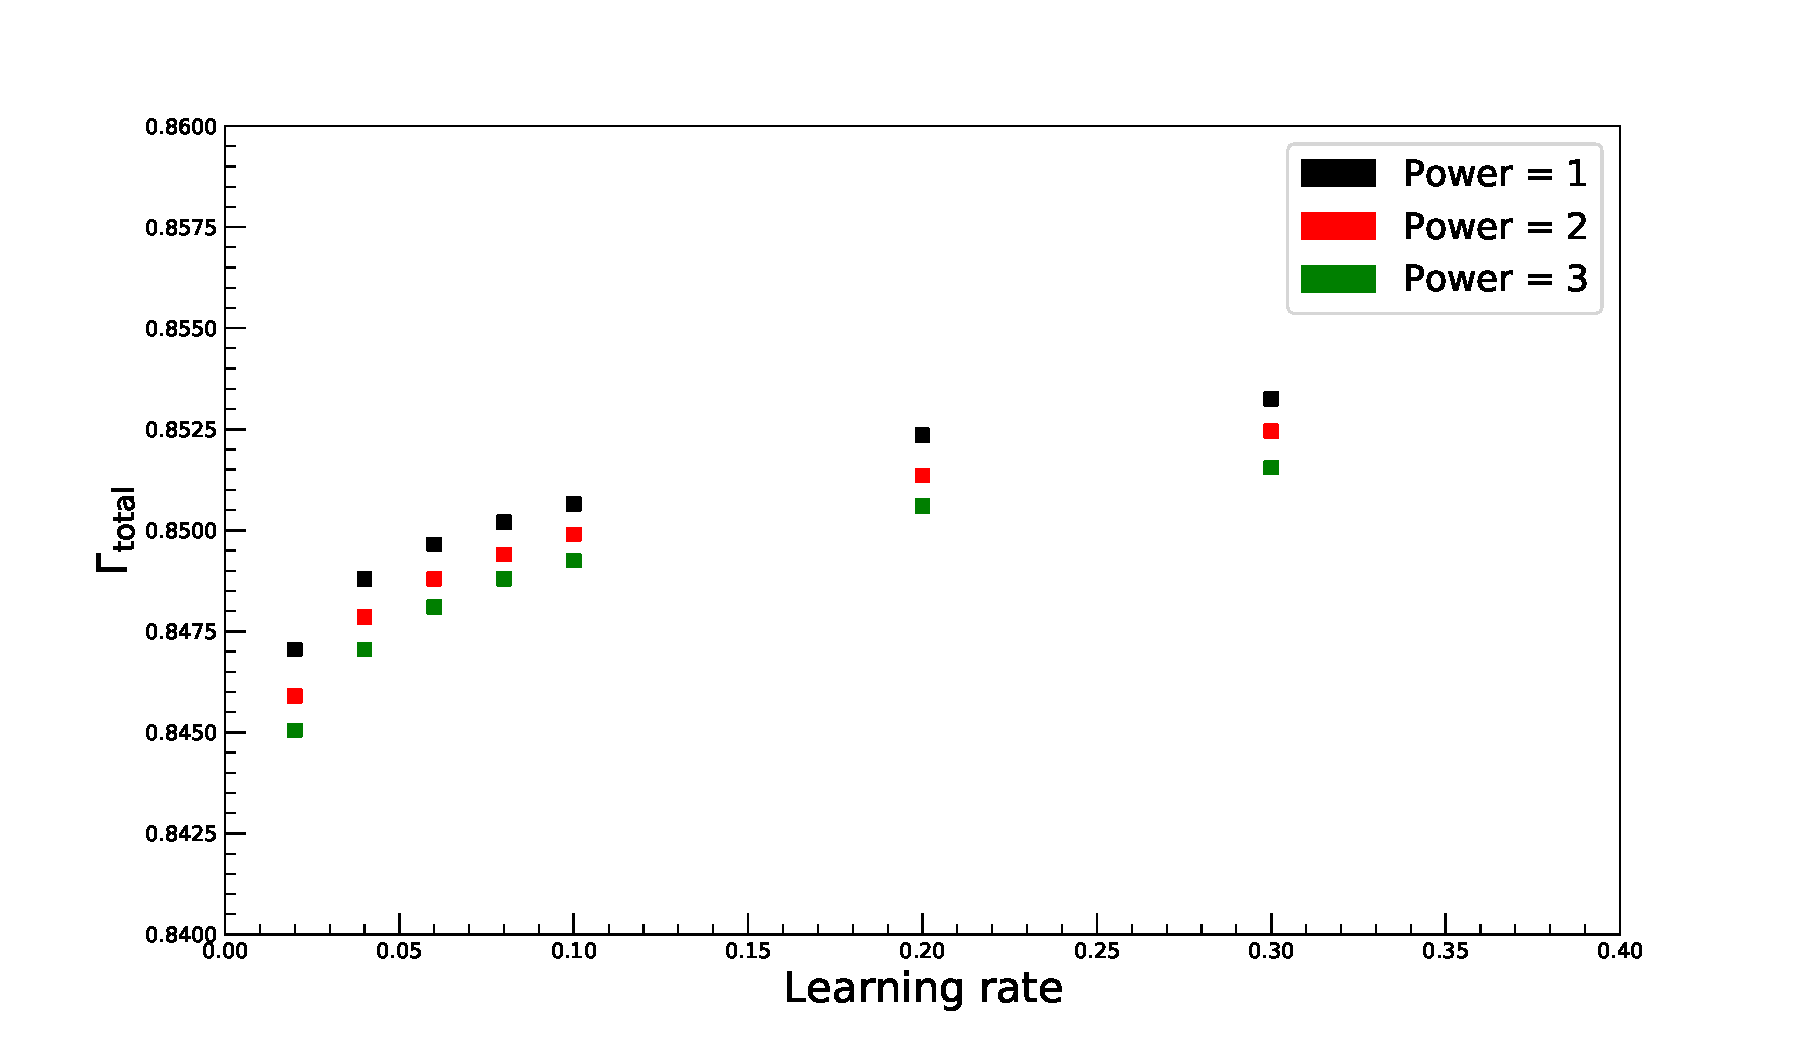
\includegraphics[width=0.93\linewidth]{figs/FNN/PolyAuc}
\caption{Obtained AUCs for FNNs trained using polynomial learning rate decay.}
\label{fig:PolyAuc}
\end{figure}

Figure \ref{fig:PolyAuc} shows the results of the polynomial learning rate decay.
Within the considered hyperparameter ranges, no improvement of the peak performance is observed compared to the training with fixed learning rates. Learning rate decays with polynomials of power 1 perform best among all investigated learning rates. The reason for this is not apparent and needs further investigations in the future. One drawback of polynomial learning rate decay is that Neural Networks, on average, have to be trained longer until the Epoch with the best performance is reached. However, for all learning rates considered with the exception of $Lr_{\text{int}} = 0.02$ the Epoch having the best performance is more than 5 Epochs away from $E_{\text{tot}} = 80$. The overall stability of the best AUC against different learning rates is only improved slightly (cf. Figure \ref{fig:LrAuc}). \\

\begin{figure}[H]
\centering
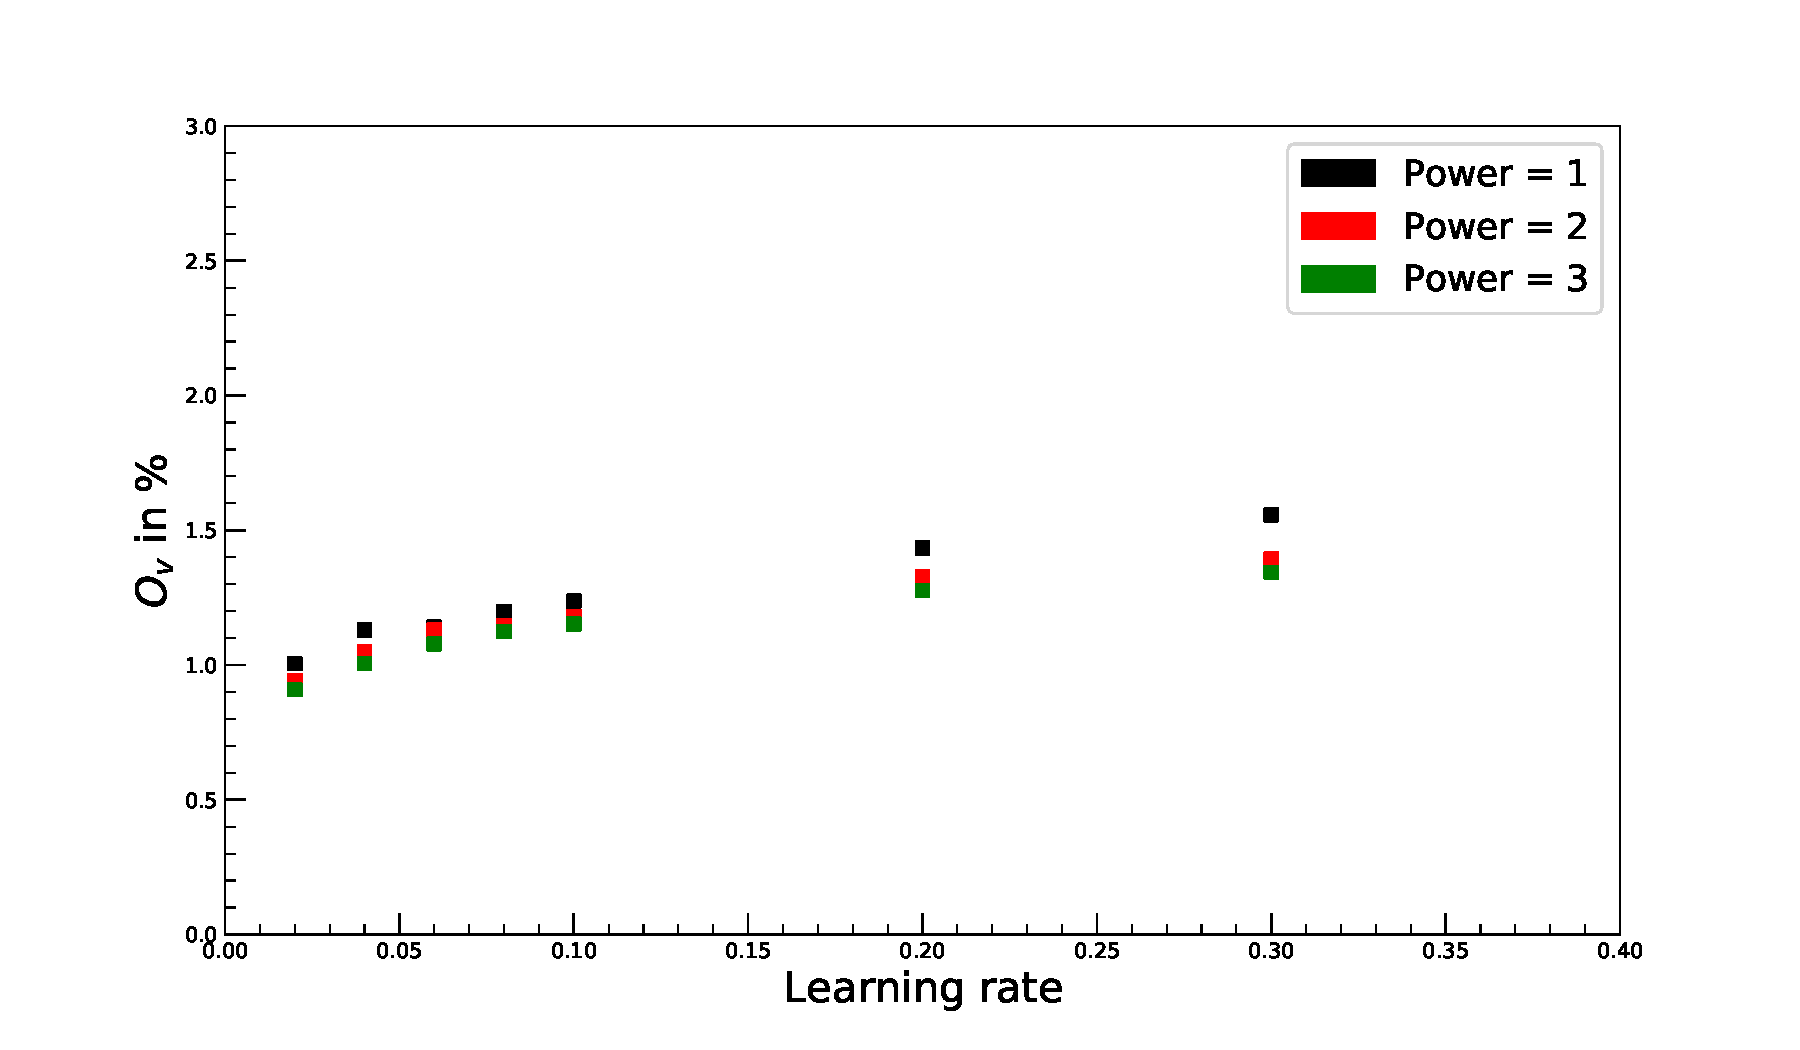
\includegraphics[width=0.93\linewidth]{figs/FNN/PolyOv}
\caption{The overtraining for FNNs trained using polynomial learning rate decay.}
\label{fig:PolyOv}
\end{figure}

The overtraining of the Neural Networks trained with polynomial learning rate decay, shown in Figure \ref{fig:PolyOv}, decreases with the learning rate and is independent of the power of the polynomial used. Similar to the overtraining observed for SGD using a fixed learning rate, all trained models have an overtraining below 1.5\%.




\paragraph{Cyclic Learning Rate Decay} \mbox{} \\

\begin{figure}[H]
\begin{subfigure}{.5\textwidth}
  \centering
  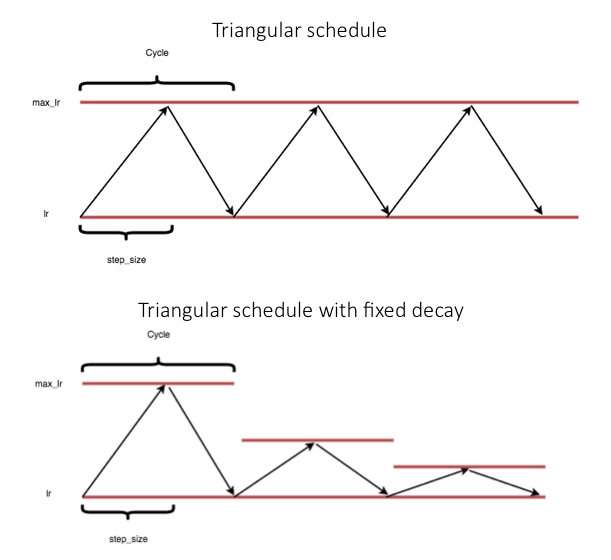
\includegraphics[width=.95\linewidth]{figs/Cycle}
  \caption{}
\end{subfigure}%
\begin{subfigure}{.5\textwidth}
  \centering
  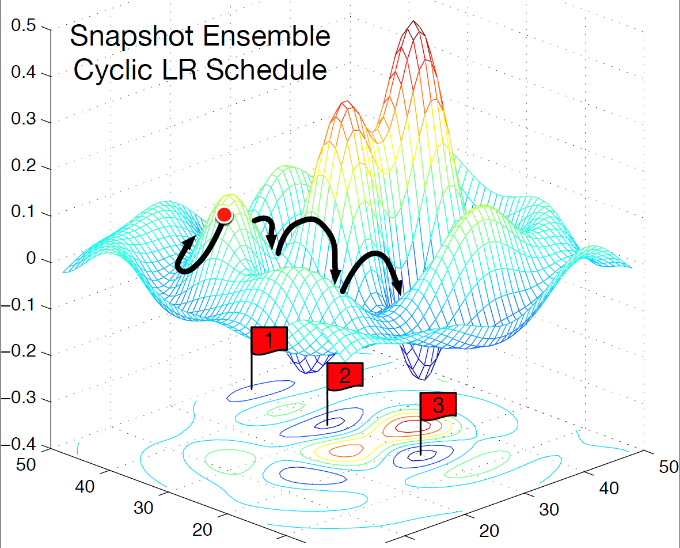
\includegraphics[width=.97\linewidth]{figs/topolgy}
  \caption{}
\end{subfigure}
\caption{a) The learning rate schedule for cyclic learning rate decay with and without additional decay of the maximum learning rate ``max\_ lr''. b) The topology of a Loss function for which cyclic learning rate decay can improve the performance of a Neural Network. The flags 1, 2 indicate the position of local minima where as flag 3 indicates the position of the global maximum. \cite{cyl1,cyl2}}
\label{fig:CylicTrain}
\end{figure}

Another attempt to improve the AUC by varying the learning rate during training is cyclic learning rate decay. The functionality is illustrated in Figure \ref{fig:CylicTrain}; during one cycle, the learning rate is linearly increased from a predefined minimum learning rate to a predefined maximum learning rate and after that linearly decreased until the minimum learning rate is reached. The number of batches needed to move from the maximum to the minimum learning rate or the other way around, is a tunable hyperparameter called \textit{stepsize}. Moreover, the maximum learning rate can be decreased after every cycle. This learning rate schedule is designed to prevent the training from getting stuck in a local minima or on a saddle points. \\
The cyclic learning rate decay study conducted 3 different parameters. The maximum learning rates considered are of the magnitude $10^{-1}$, while the minimum learning rates are of the magnitude $10^{-2}$. Simultaneously 5 different stepsizes are considered, which are chosen close to the suggested $2-8$ iterations per Epoch ($\sim 160 - 640$) in \cite{stepsize}. Each combination is trained with a static maximum learning rate and a maximum learning rate that decreased to its half value after each cycle. All other parameters are the same parameters used for the previous learning rate study. \\

\begin{figure}[H]
\centering
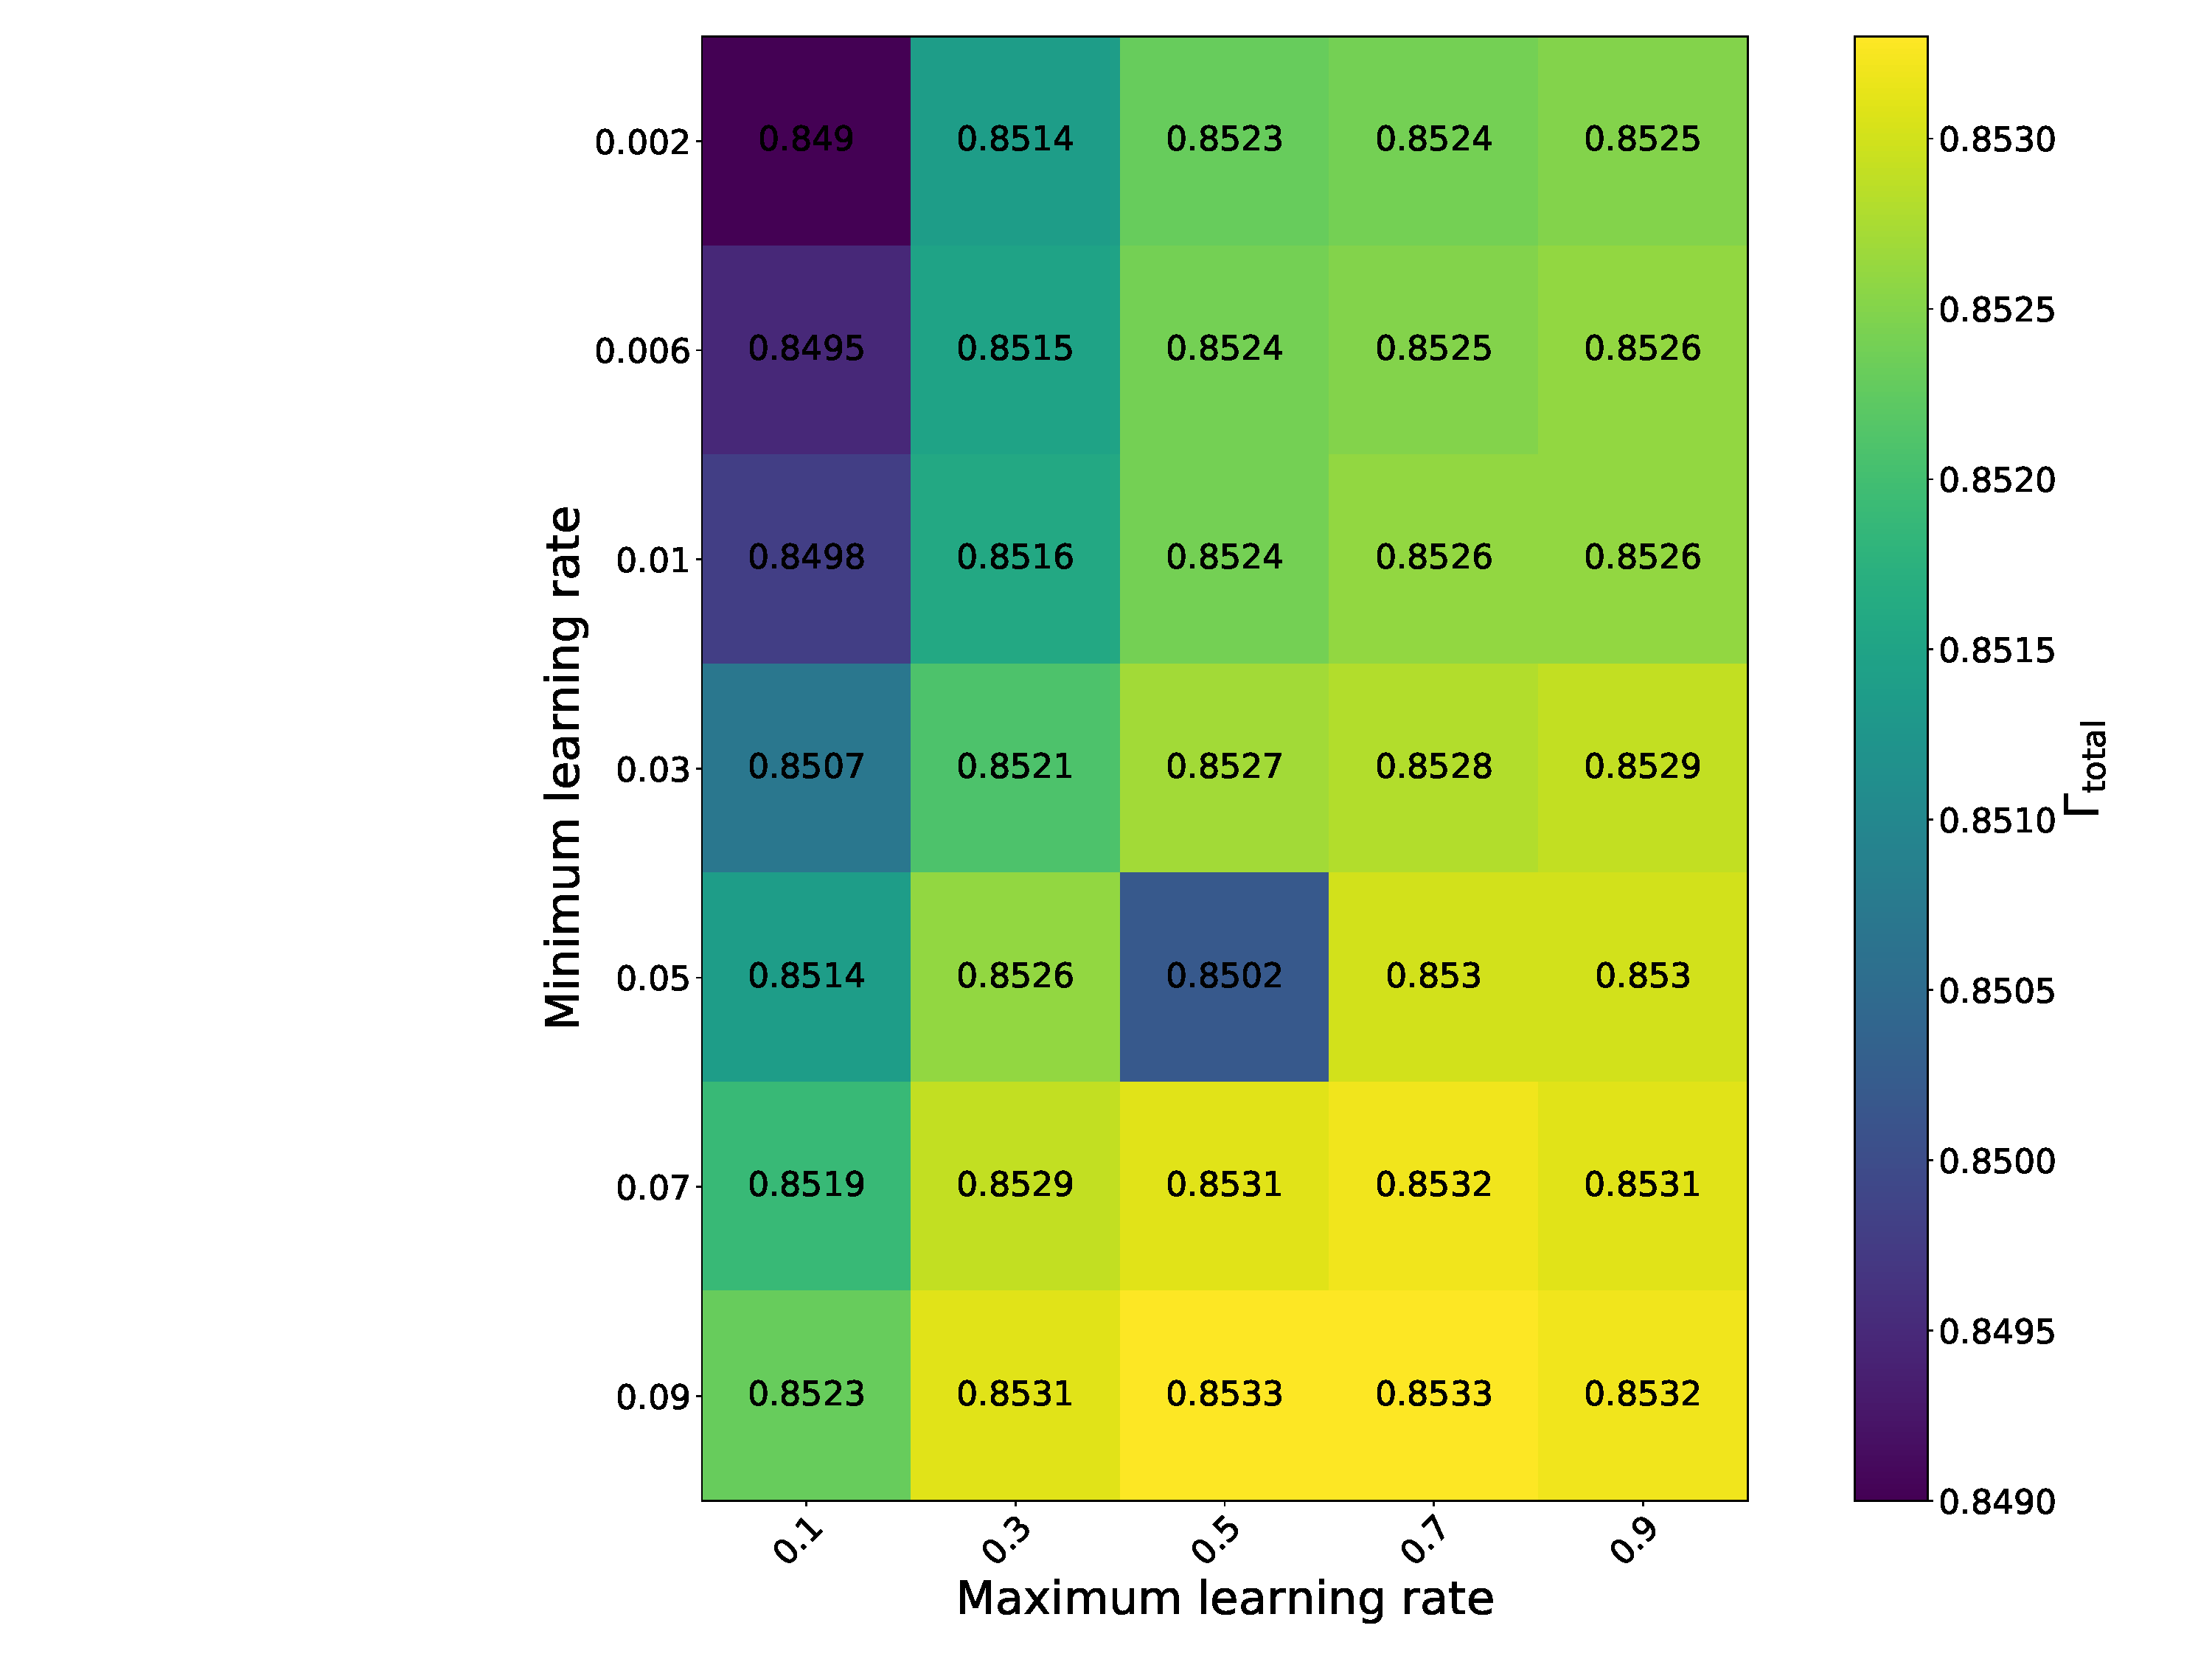
\includegraphics[width=\linewidth]{figs/FNN/Heat_MinMax}
\caption{The dependence between the maximum and the minimum learning rates of FNNs trained with cyclic learning rate decay.}
\label{fig:CylicHeatLr}
\end{figure}

\vspace{-0.1cm}

The heatmap in Figure \ref{fig:CylicHeatLr} shows the results obtained for the different combinations of minimum and maximum learning rates where the quoted $\Gamma_{\text{total}}$ values are the average AUC over all stepsizes for both the fixed and the decaying maximum learning rate training. Varying the minimum learning rate improves the performance of the Neural Networks more than varying the maximum learning rate. Therefore, no second minimum that results in a better performance is found. The drop in performance obtained for models trained with a maximum learning rate of 0.1 is most likely not an indication for a local minimum but rather due to the fact that the training did not converge during 120 Epochs. For minimum learning smaller than 0.3, the same problem occurred.  Similar to polynomial learning rate decay, Neural Networks trained with cyclic learning rate decay need more Epochs to until the best performance is found compared to Neural Networks trained with a fixed learning rate. \\
The comparison between cyclic learning rate decay with fixed maximum learning rate and with additional decay of the maximum learning rate is shown in Figure \ref{fig:CylicLr} where only the 5 best-performing Neural Networks were considered for each learning rate. No significant difference between the two learning schedules (red and black squares) is observable. \\

\begin{figure}[H]
\centering
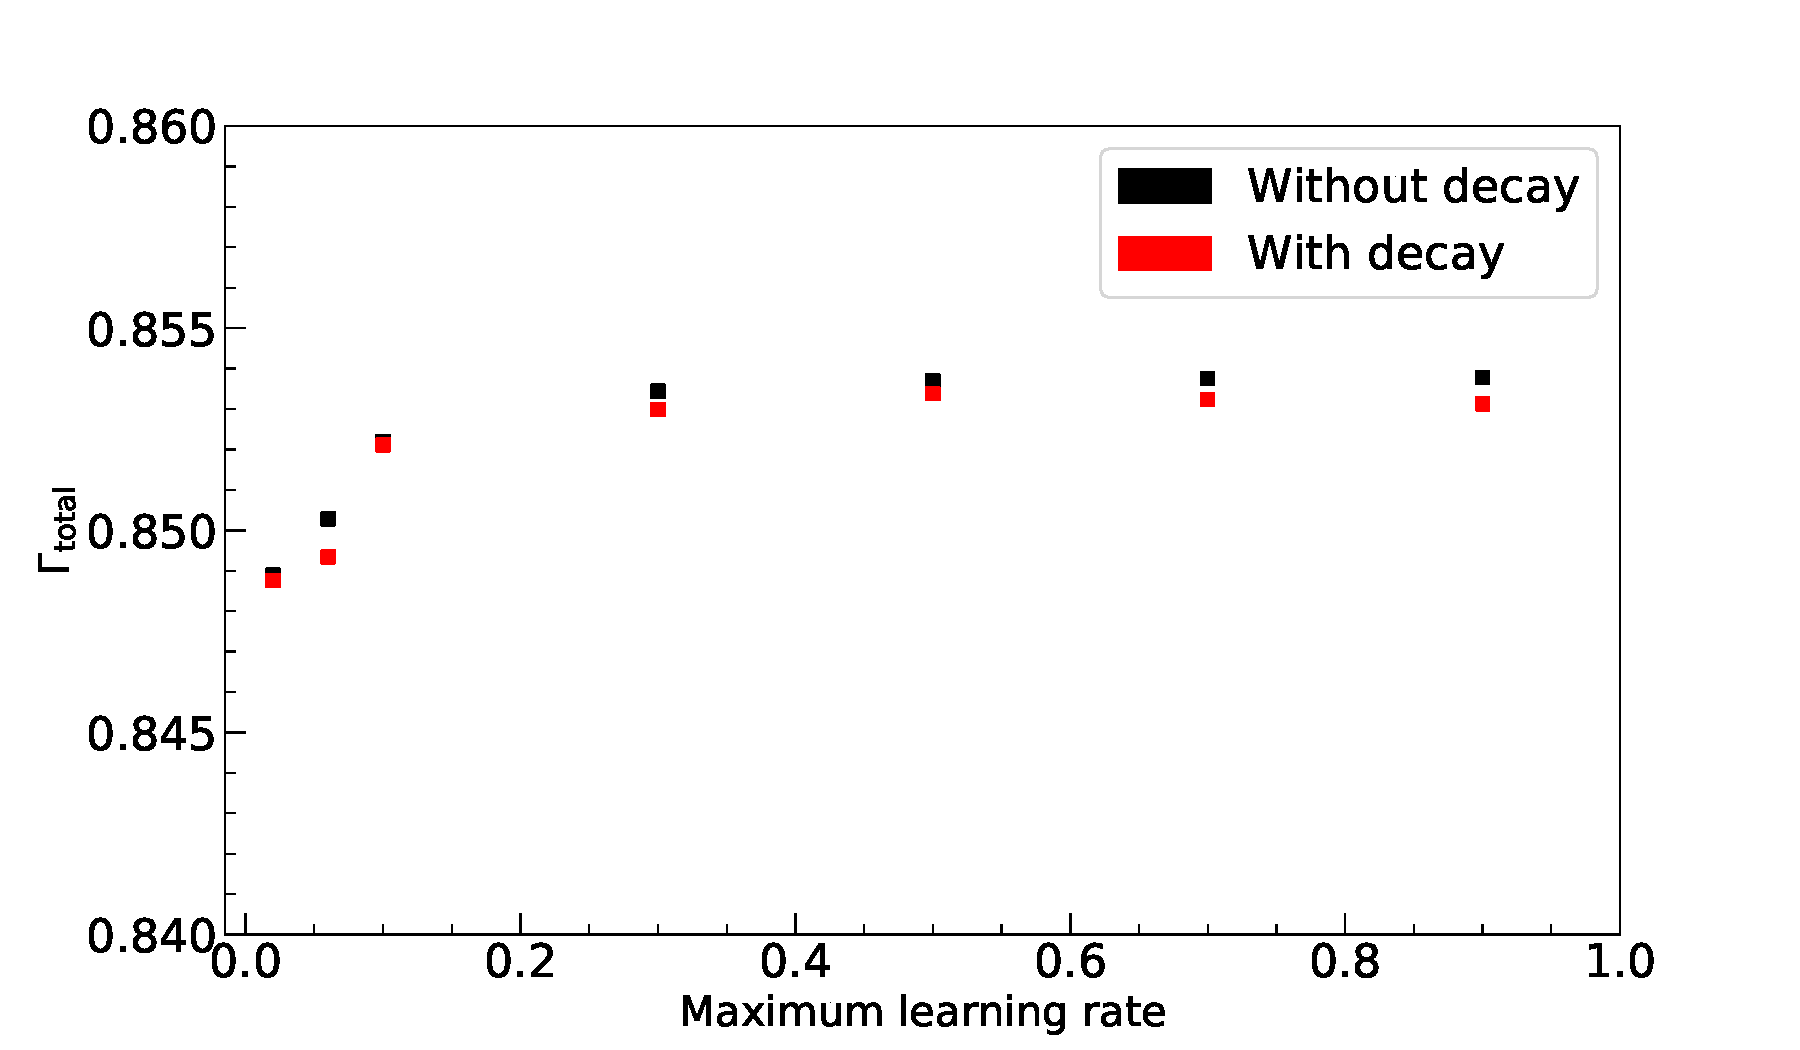
\includegraphics[width=0.95\linewidth]{figs/FNN/MaxAuc_Fixed}
\caption{The observed AUCs for different maximum learning rate using cyclic decay with and without additional decay.}
\label{fig:CylicLr}
\end{figure}

\begin{figure}[H]
\centering
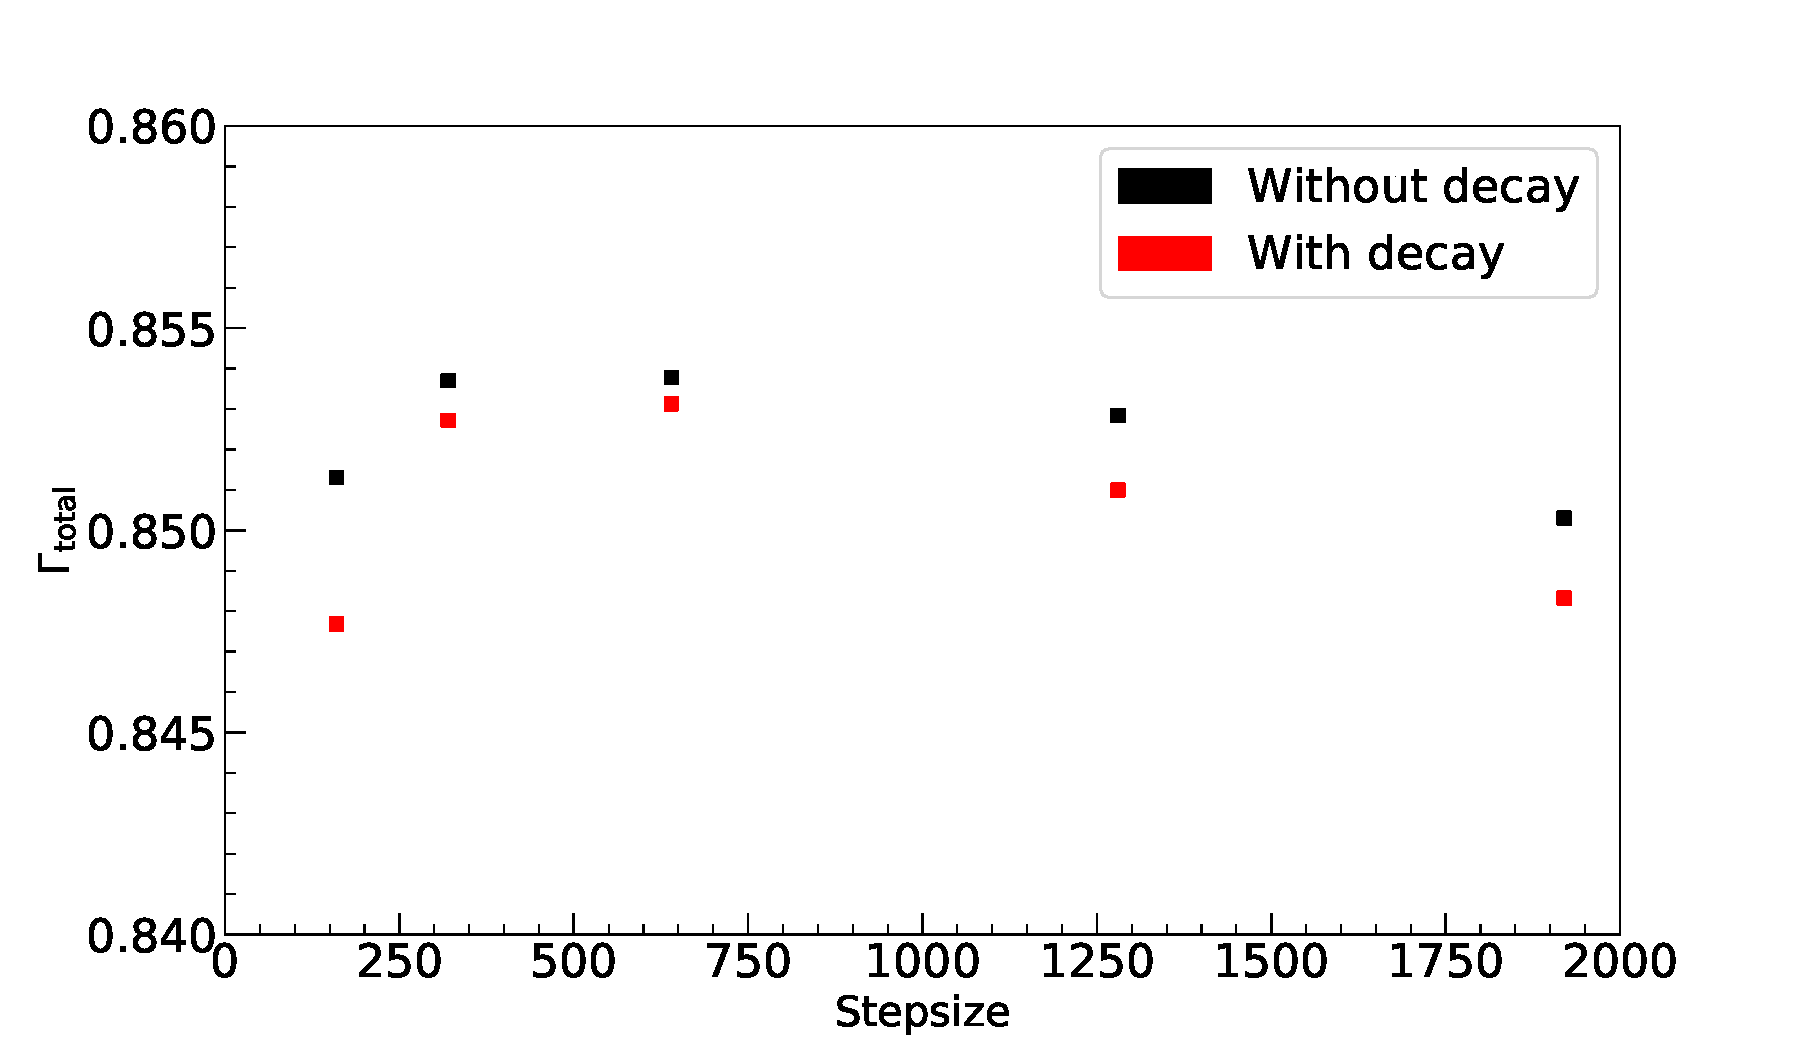
\includegraphics[width=0.95\linewidth]{figs/FNN/StepAuc_Fixed}
\caption{The dependence of the AUC on the stepsize chosen for the cyclic learning rate decay.}
\label{fig:CylicStepSize}
\end{figure}

Figure \ref{fig:CylicStepSize} shows obtained AUCs for the diverse stepsizes and different types of learning schedules. Stepsizes in the recommended region (between 160-640) result in the best AUCs while stepsizes below or above tend to decrease performance. The difference in performance between Neural Networks trained with the two distinctive learning rate schedules is small for stepsizes in the recommended region. Outside of the region, training without additional decay of the maximum learning rate works better. \\
The Neural Network with the best performance uses a constant maximum learning rate of 0.9, a minimum learning rate of 0.03, and a stepsize of 640. The obtained $\Gamma_{\text{total}}$ is 0.854 with an overtraining of 1.7\%.


\paragraph {Regularization} \mbox{} \\

The study of regularization aims to increase the AUC obtained on the testing dataset by decreasing the overtraining. Obtained models with under 2\% overtraining are already below the point of exceptions (5\%), and thus it is unlikely to obtain a higher AUC. \\
The two methods applied are the Dropout, govern by the probability $p$ for a neuron to be ignored during training and the Ridge regression, govern by $\alpha$ the scaling parameter of the additional Loss function term. The investigated values for $\alpha$ range from 0.001 (small regularization) to 0.1 (strong regularization) while the probability of Dropout is either 20\%, 40\%, or 60\%. The Dropout is only applied to the neurons in the hidden layer, giving the Neural Network the possibility of recovering performance during the training. To investigate the correlation between the learning rate and the different regularization methods, 5 different fixed learning rates between 0.0005 and 0.01 are investigated. The selected optimization algorithm is Adam since this optimization algorithm was used for the best-performing Neural Network in the fixed learning rate study. \\

\begin{figure}[H]
\centering
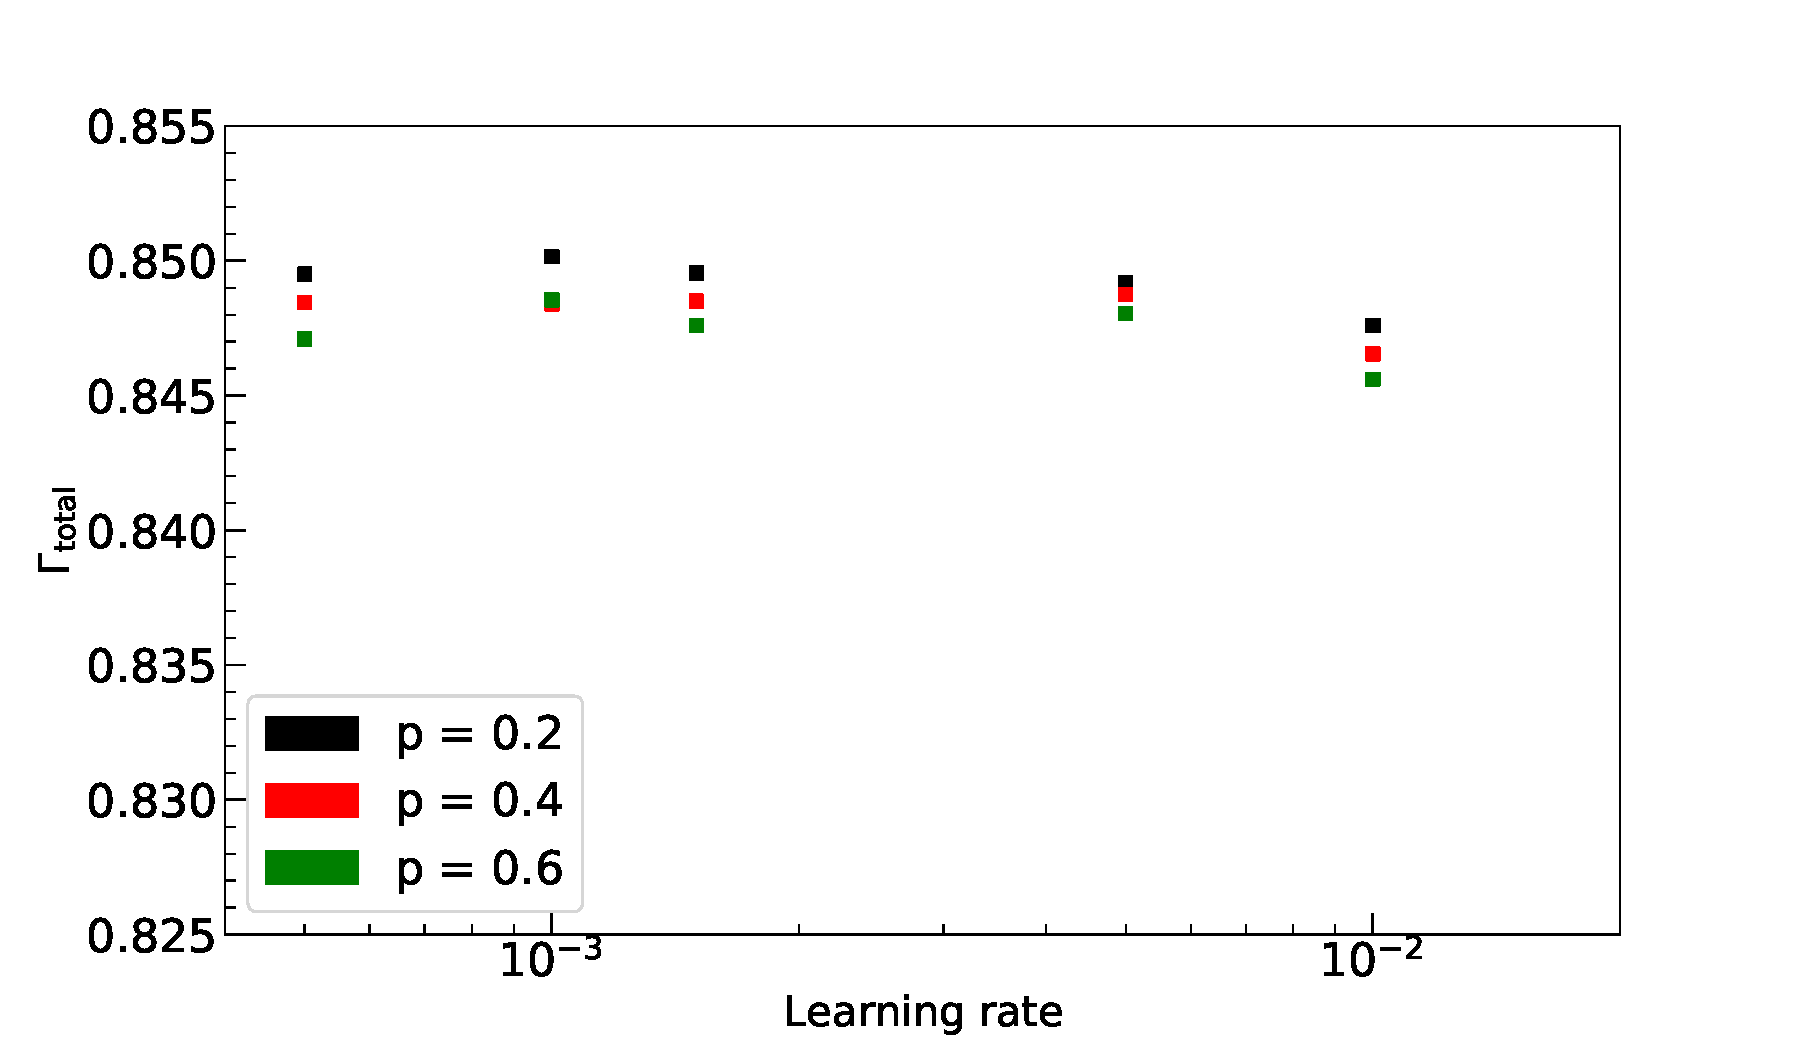
\includegraphics[width=\linewidth]{figs/FNN/Drop_Fixed}
\caption{Obtained AUCs for different learning rates and distinct choices of $p$, the Dropout probability.}
\label{fig:ReguDrop}
\end{figure}

Figure \ref{fig:ReguDrop} shows the obtained AUCs for the different learning rates and Dropout values, where $\alpha$ was fixed to 0.001. The peak performance has decreased by 0.003 compared to the results obtained without any regularization (cf. Figure \ref{fig:LrAuc}). Neural Networks with a lower probability of Dropout outperform those with a higher probability of Dropout as is to be expected for a regularization method. This behavior is also apparent in Figure \ref{fig:Regu}, where the learning rate is fixed to 0.001. The performances decrease continuously from the top left corner, where only little regularization is applied to the bottom right corner, where a strong regularization is applied. The overtraining of the trained Neural Networks, shown in Figure \ref{fig:ReguOv}, decreases with the amount of regularization applied as intended. \\
In the investigated parameter range, a large Ridge regression term is a stronger restriction than dropping out neurons in the first hidden layer with a high probability.

\begin{figure}[H]
\begin{subfigure}{.5\textwidth}
  \centering
  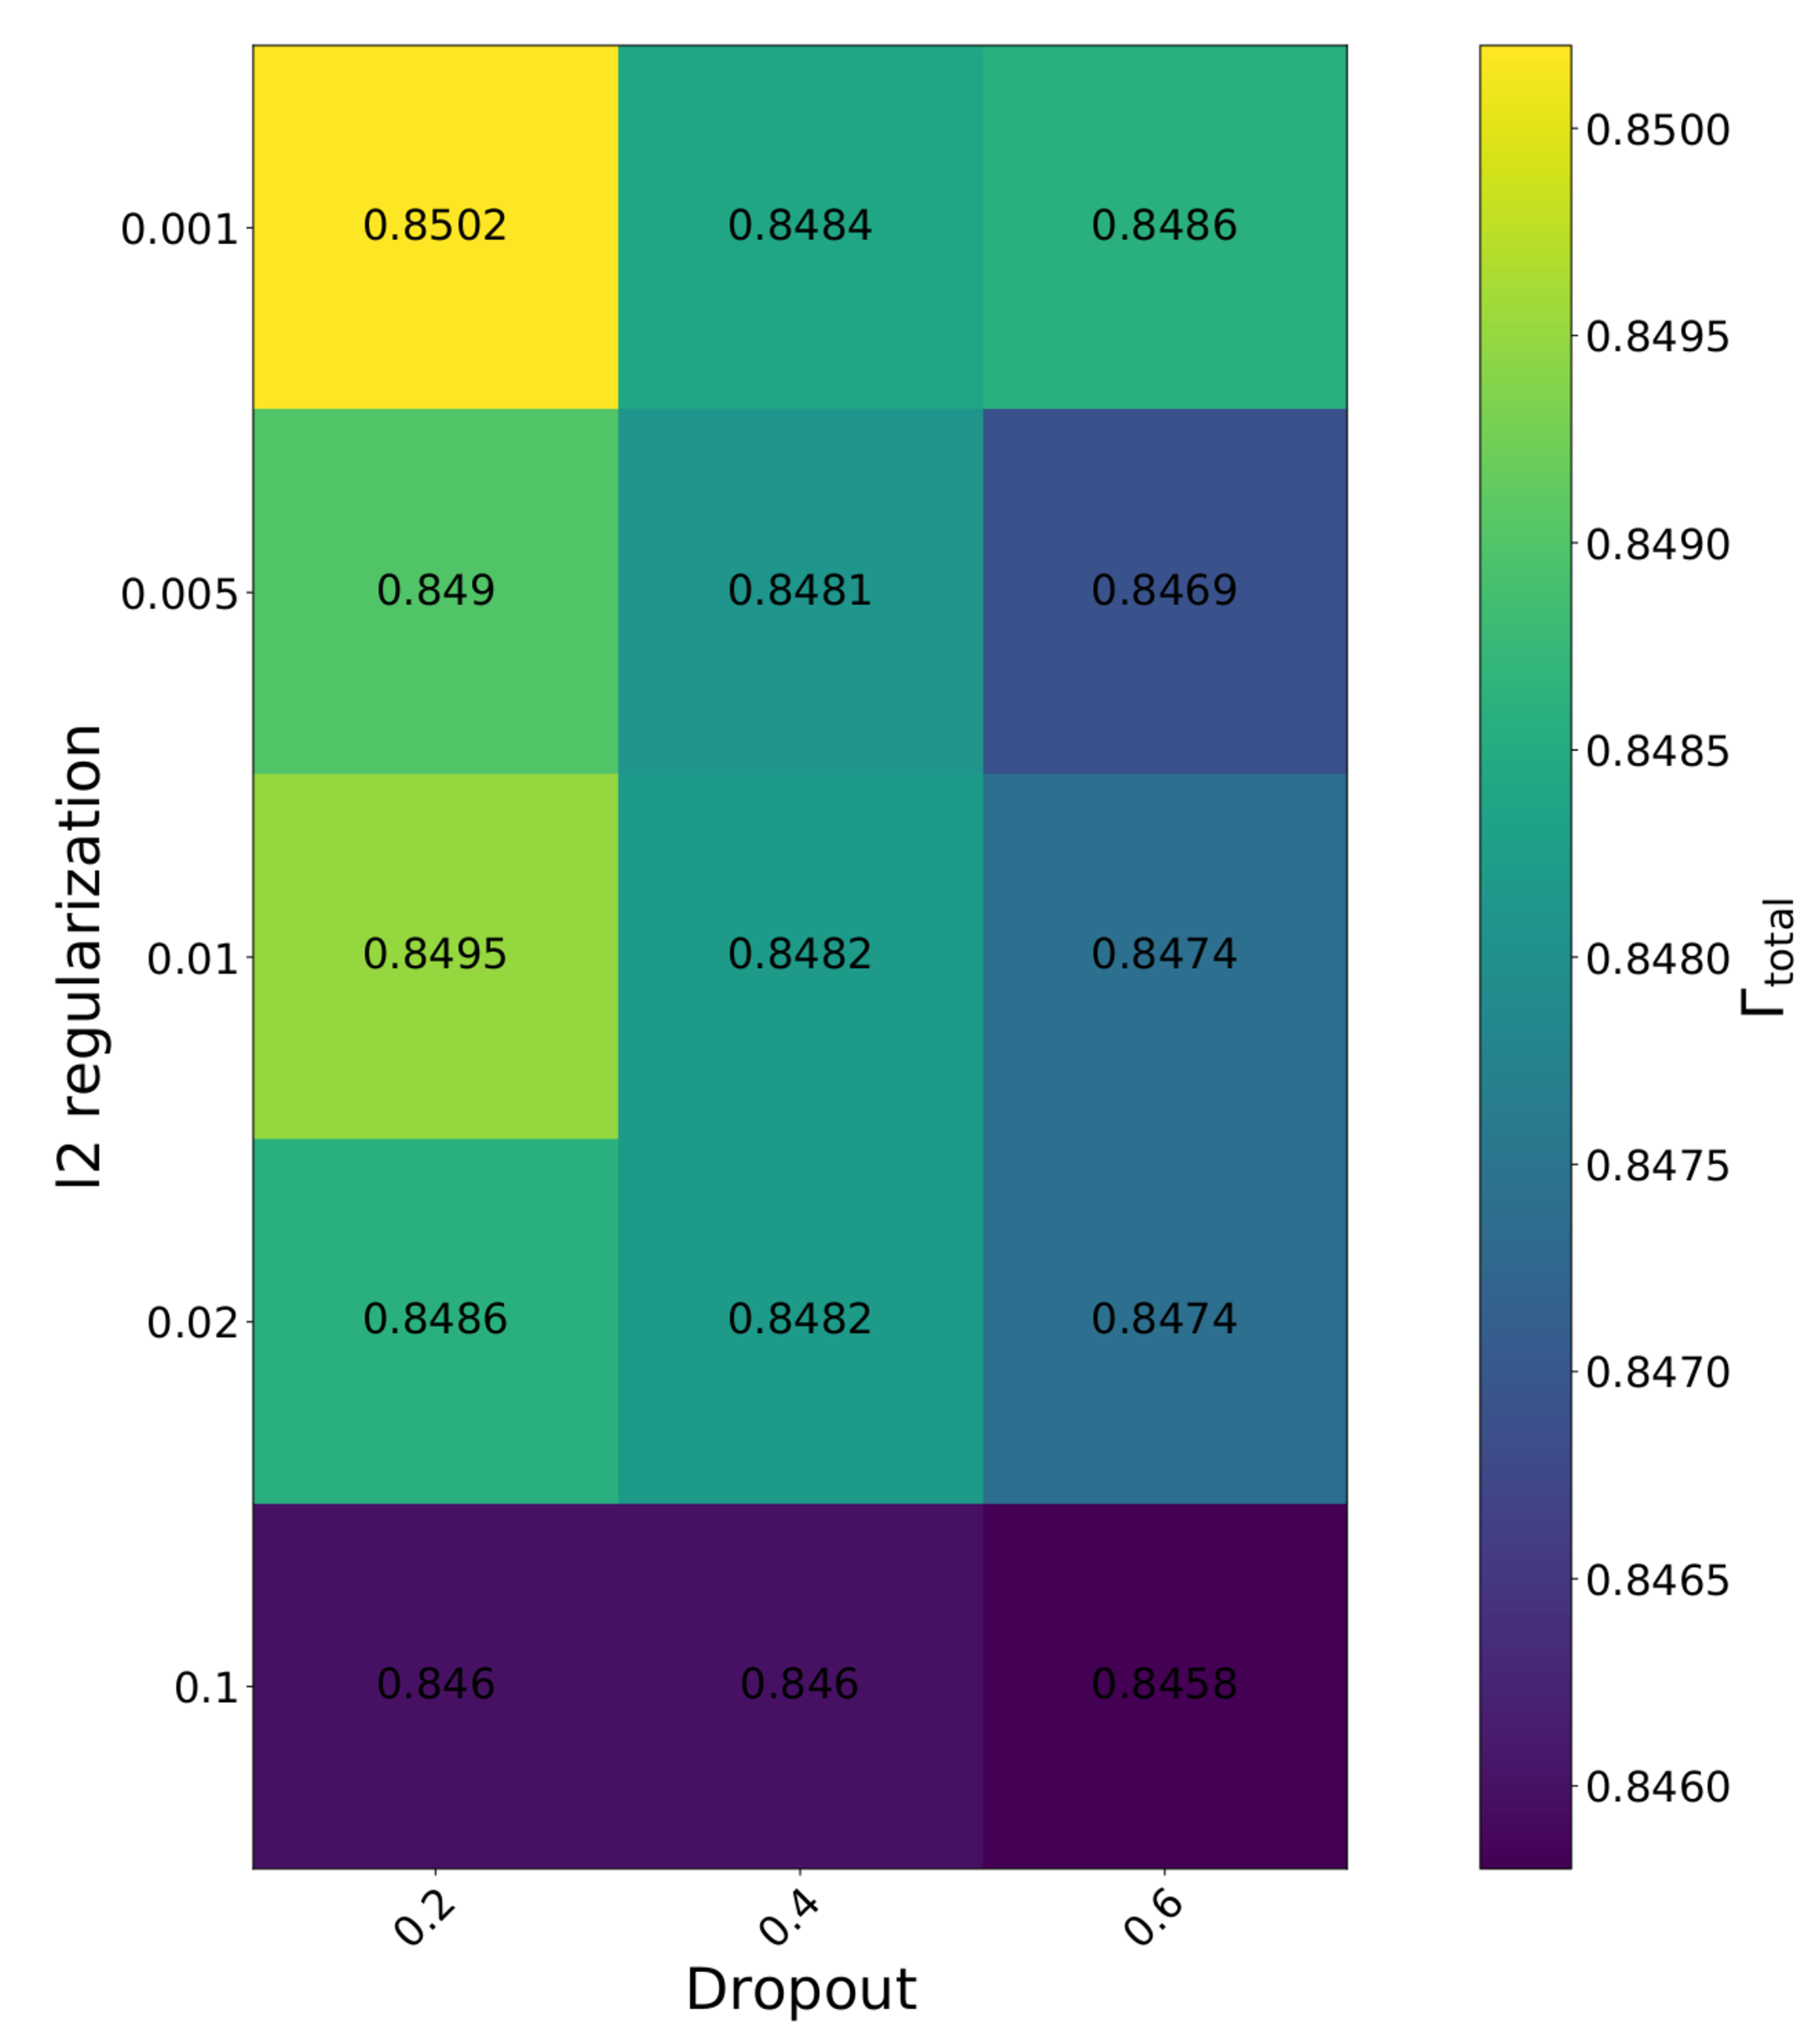
\includegraphics[width=.99\linewidth]{figs/FNN/Heat_l2DropAuc}
  \caption{}
  \label{fig:ReguLr}
\end{subfigure}%
\begin{subfigure}{.5\textwidth}
  \centering
  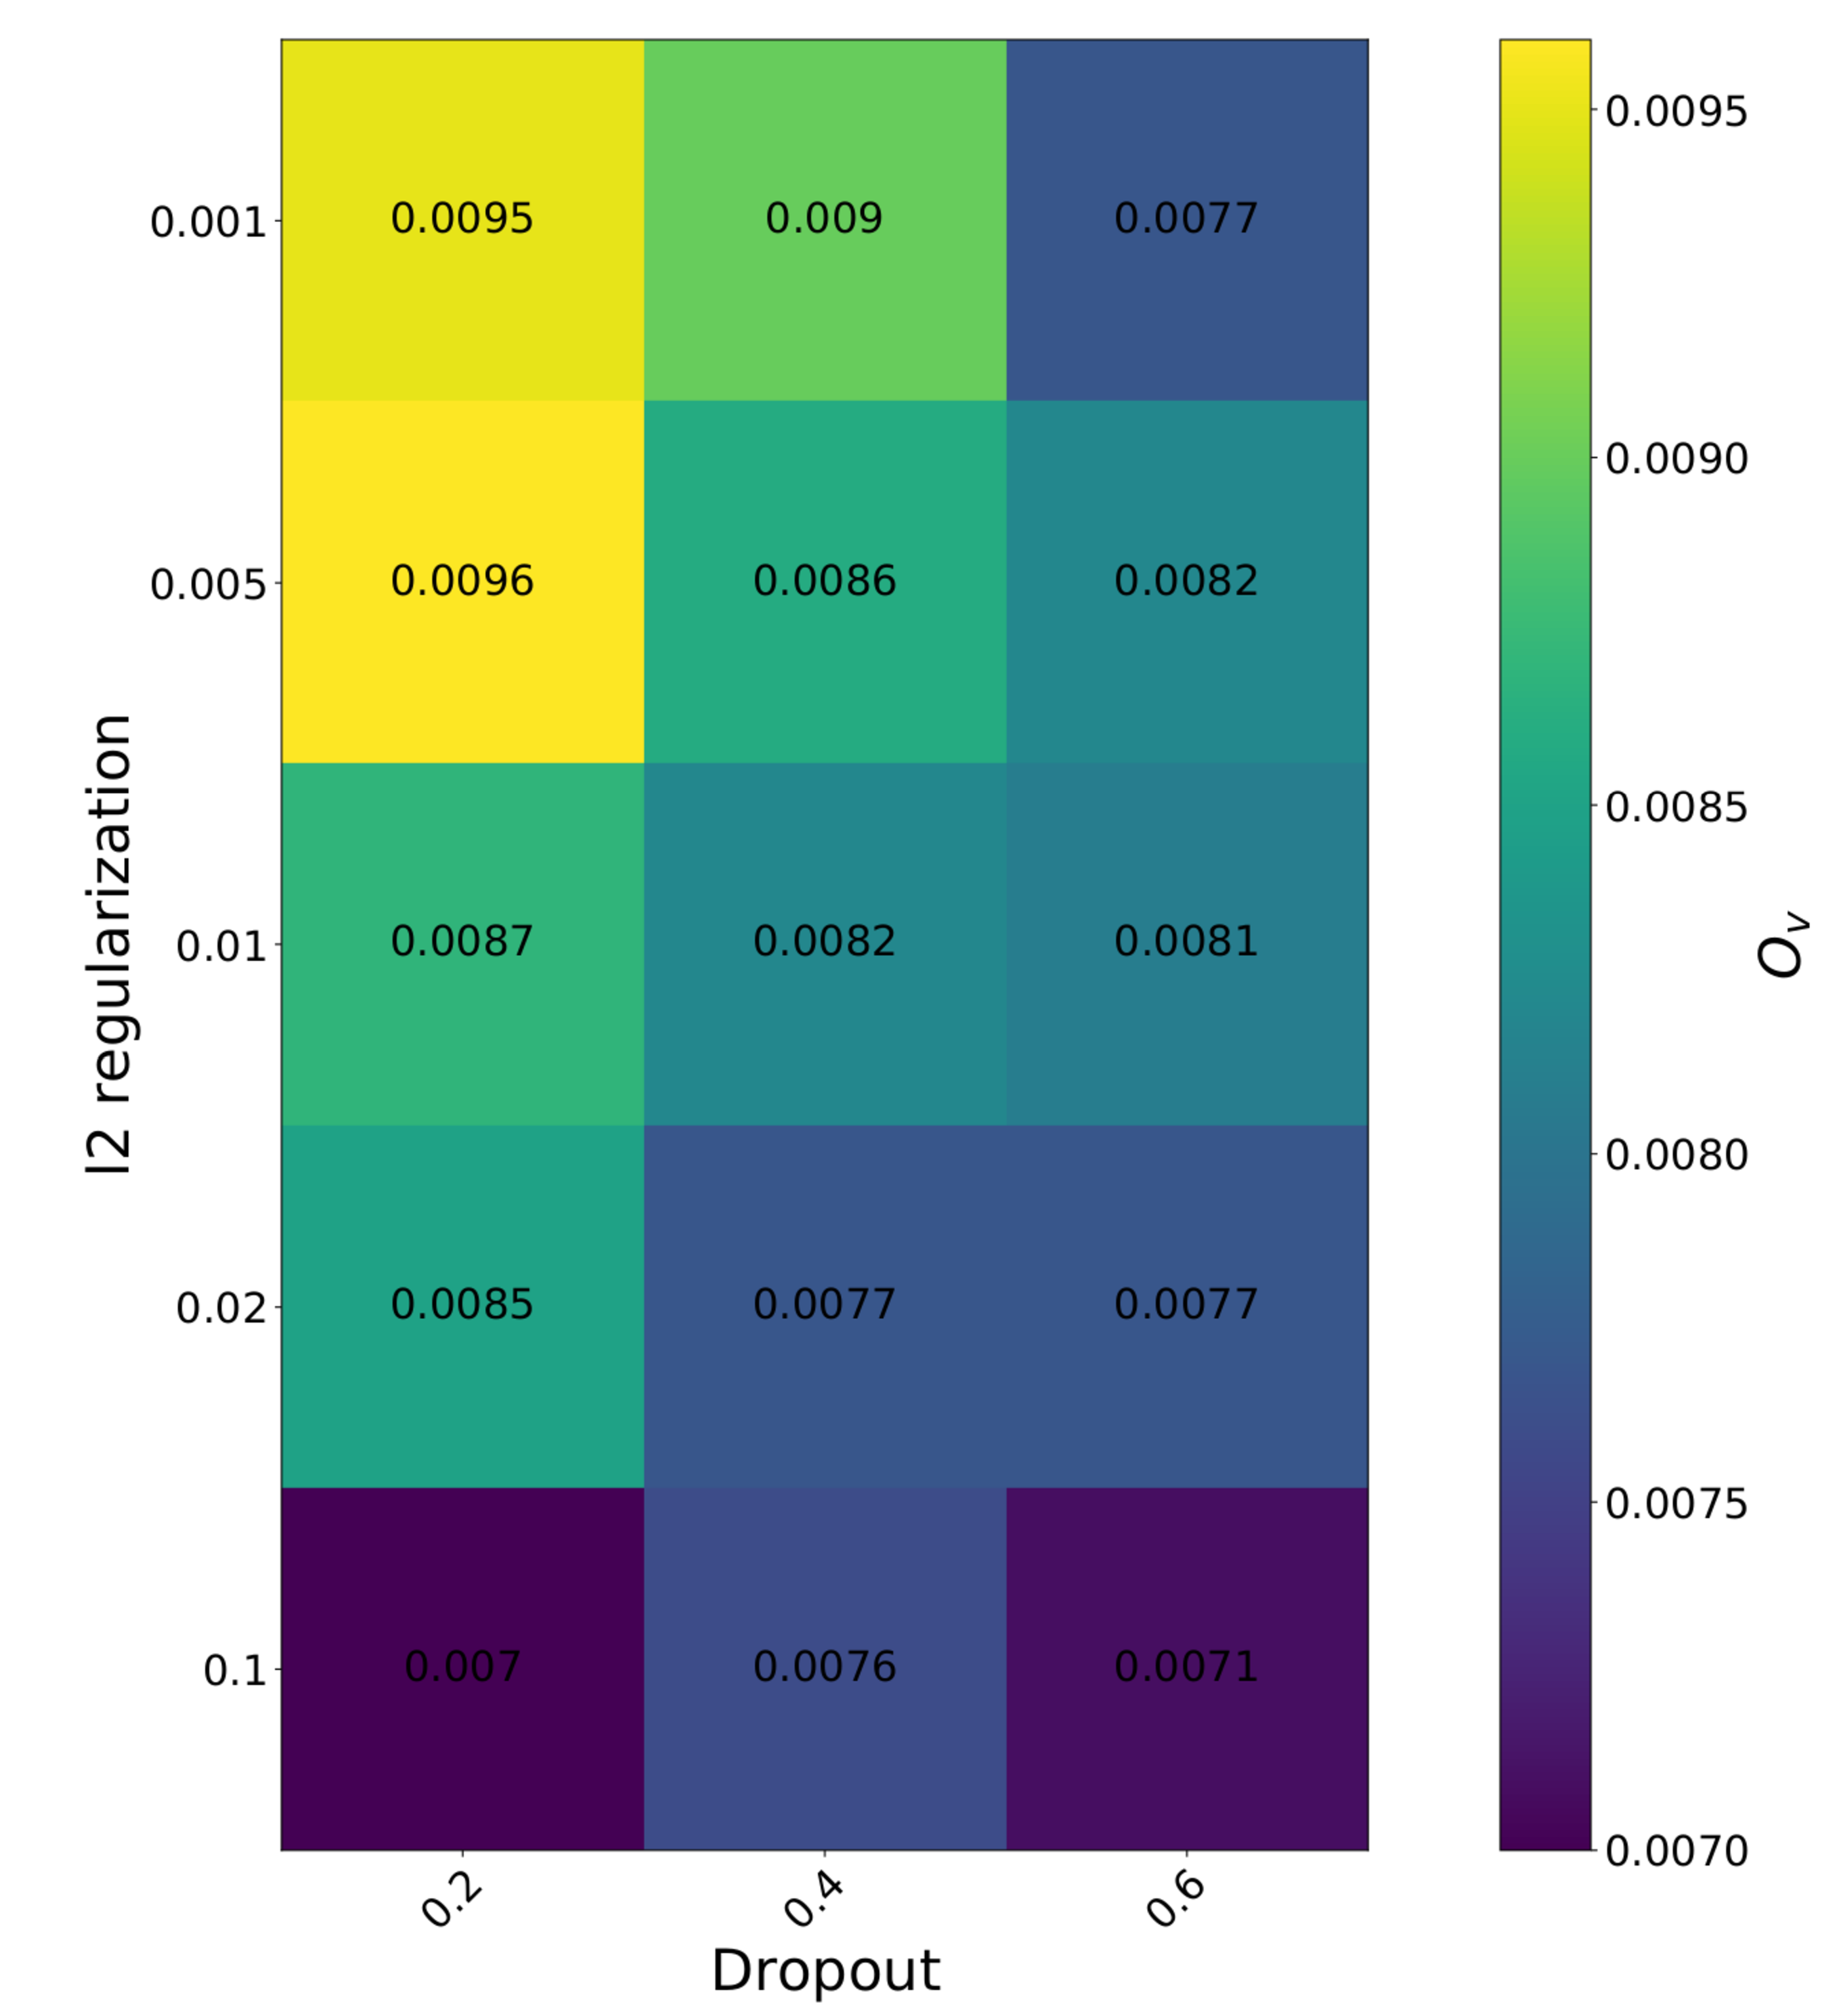
\includegraphics[width=.99\linewidth]{figs/FNN/Heat_l2DropOv}
  \caption{}
  \label{fig:ReguOv}
\end{subfigure}
\caption{The dependence of the AUC (a) and the overtraining (b) for different Dropout probabilities and l2 (Ridge) regularization.}
\label{fig:Regu}
\end{figure}


\paragraph{Achieved Separation} \mbox{} \\

\begin{figure}[H]
\begin{subfigure}{.5\textwidth}
  \centering
  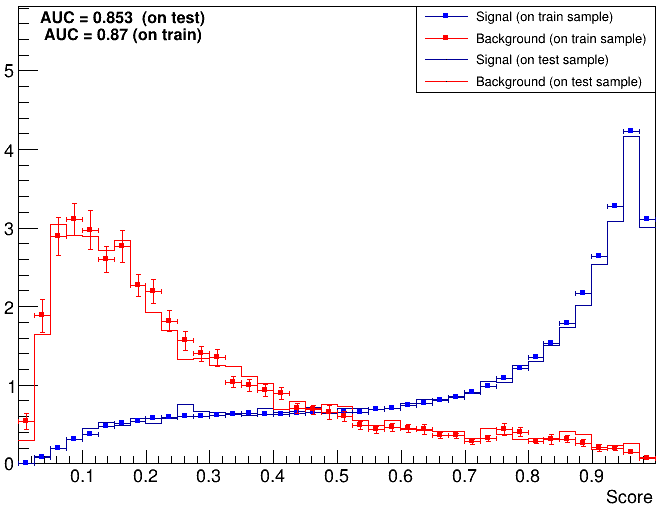
\includegraphics[width=.99\linewidth]{figs/FNN/ScoreFNN19Even}
  \caption{}
  \label{fig:ScoreEven}
\end{subfigure}%
\begin{subfigure}{.5\textwidth}
  \centering
  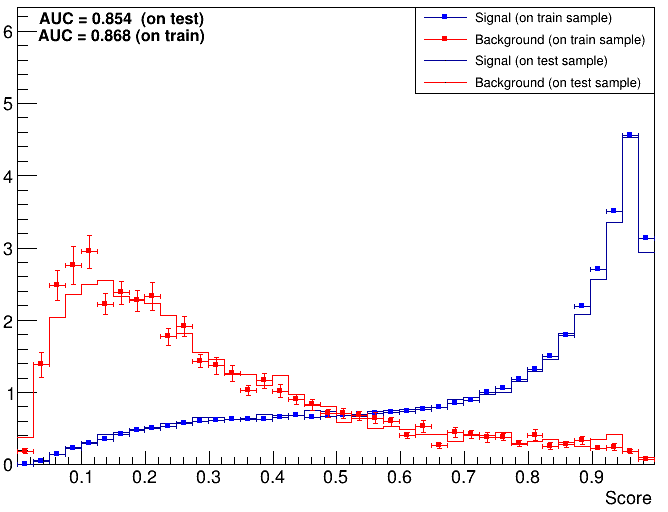
\includegraphics[width=.99\linewidth]{figs/FNN/ScoreFNN19Odd}
  \caption{}
  \label{fig:ScoreOdd}
\end{subfigure}
\caption{Observed Neural Network scores for the Neural Network trained with the background dataset containing even event numbers (a) and on the background dataset constraining odd event numbers (b).}
\label{fig:Scores}
\end{figure}

The Neural Network obtained in the sub-section about cyclic learning rate decay is the best-performing model obtained for the $t\bar{t}t\bar{t}$ application. The score for the training on the dataset containing the background events with even event numbers is shown in Figure \ref{fig:ScoreEven}, whereas the score for the training on the dataset containing the background events with odd event numbers is shown in Figure \ref{fig:ScoreOdd}. Both classifications assign most signal events to scores above 0.7, and background events scores below 0.5. This indicates that the Neural Network is better at identifying signal events than at identifying background events, which is expected since the background dataset contains many different processes. The distance in each bin between the dots and the solid lines is related to the overtraining of the model. Since the Neural Network used has a tiny overtraining, most dots and lines are very close. \\

\begin{figure}[H]
\begin{subfigure}{1\textwidth}
  \centering
  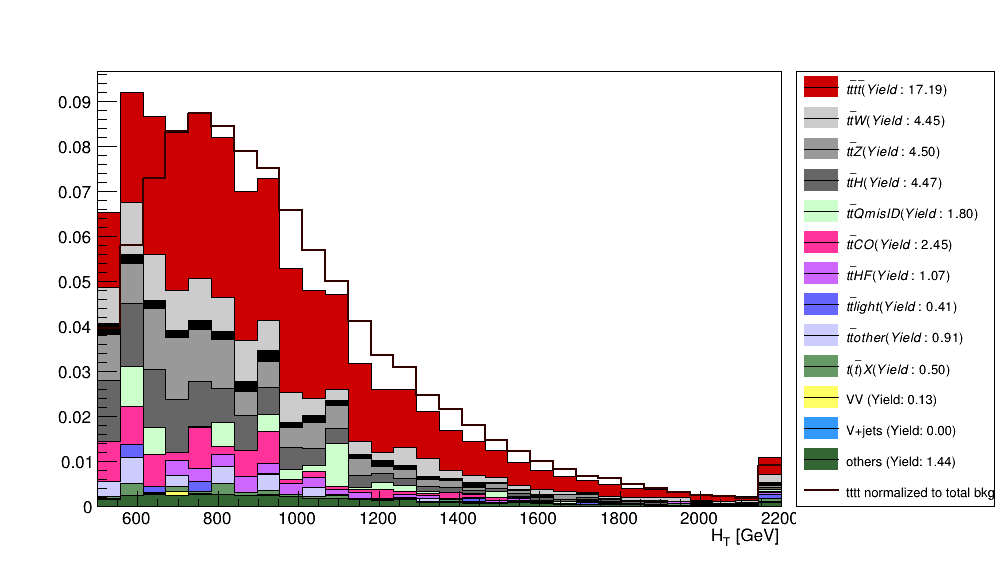
\includegraphics[width=.93\linewidth]{figs/FNN/HT_all_Even}
  \caption{Dataset with even numbered background events}
  \label{fig:HTEven}
\end{subfigure} \\
\begin{subfigure}{1\textwidth}
  \centering
  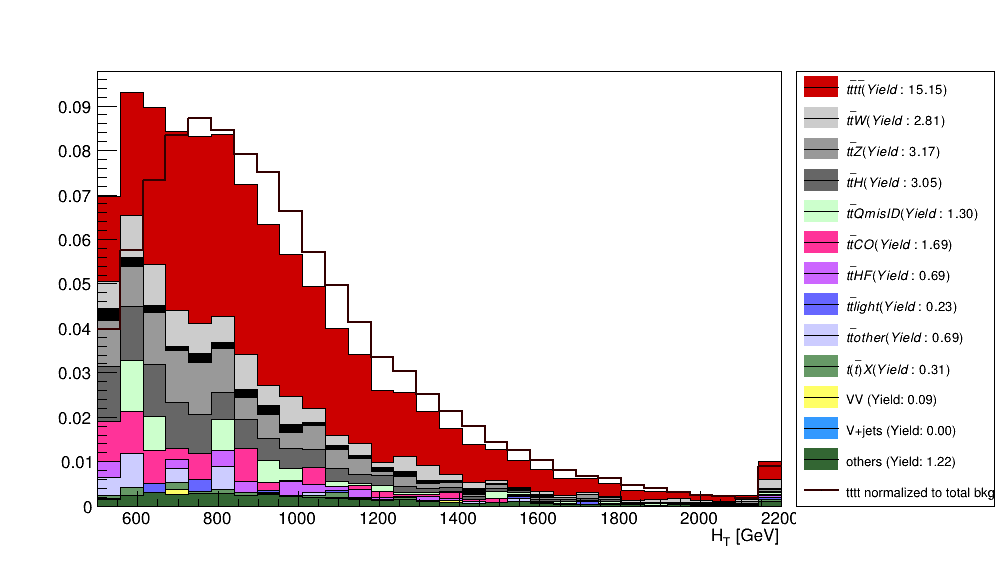
\includegraphics[width=.93\linewidth]{figs/FNN/HT_all_Odd}
  \caption{Dataset with odd numbered background events}
  \label{fig:HTOdd}
\end{subfigure}
\caption{$H_{\text{T}}$ distributions after applying a cut (optimized on the signal efficiency) to the FNN scores obtained for the training on the background dataset containing even event numbers (a) and the background dataset constraining odd event numbers (b). The last bin additionally contains all events with $H_{\text{T}} > 2200$.}
\label{fig:HTFNN}
\end{figure}

To investigate which backgrounds are particularly hard to separate from the $t\bar{t}t\bar{t}$, a cut on the scores is optimized based on the signal efficiency. For both trainings the optimal cut is determined to be 0.7 which increases the signal efficiency in the signal region from 1.8 to 3.0. The $H_{\text{T}}$ distributions for the two cases are shown in Figure \ref{fig:HTFNN}. The dominant backgrounds after applying the cut are still $t\bar{t}W$, $t\bar{t}Z$ and $t\bar{t}H$. The model trained on the backgrounds with even event numbers is better in rejecting $t\bar{t}CO$ while the model trained on the backgrounds with odd event numbers is better in rejecting $t\bar{t}$others. However, the difference is minor and therefore most likely a coincidence. The rejection of all other backgrounds is approximately equally good for both setups when normalized to the signal yield in the investigated region. The signal yield is reduced by a factor of 2 while most other backgrounds are reduced by a factor of $\sim 25$. The background  yield of the dataset ``others'' mainly containing $t\bar{t}t$ is the background that is hardest to distinguish from $t\bar{t}t\bar{t}$ and is only reduced by a factor of 3. A similar result was obtained by the BDT used in the official ATLAS $t\bar{t}t\bar{t}$ analysis at $\sqrt{s} = \SI{13}{TeV}$ which used the same datasets. In fact, for the high BDT region a significant $t\bar{t}t$ contamination was observed. This can be especially problematic because the $t\bar{t}t$ cross section, is only known at leading order $\sigma_{t\bar{t}t} = \SI{1.9}{fb}$ (at $\sqrt{s} = \SI{14}{TeV}$) \cite{3t}. If the  $\sigma_{t\bar{t}t}$ at NLO is higher than the LO cross section $t\bar{t}t$ could become the dominant background for $t\bar{t}t\bar{t}$. \\

\paragraph{Validation and Error Estimation} \mbox{} \\

\begin{figure}[H]
\centering
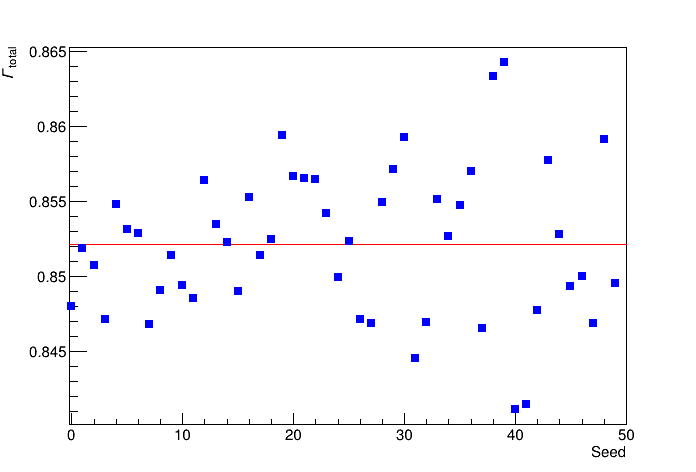
\includegraphics[width=\linewidth]{figs/FNN/BootStrap}
\caption{AUCs observed by using the bootstrap method on the validation set. The seed quoted (times 365) is the random seed used to generate the different resampled versions of the validation set. The red line indicates the mean of all observed AUCs.}
\label{fig:BootStrapFNN}
\end{figure}

As mentioned preciously in Section \ref{sec:splitting} the generalization of the optimized Neural Network has to be validated on the restrained validation dataset. The error of observed AUC can than be obtained by boostrapping. The selected number of resampled datasets is 50. \\
The bootstrapping results for the selected Neural Network performed on the validation set is shown in Figure \ref{fig:BootStrapFNN}. The seed quoted on the x-axis is the random seed (times 365) used for resampling the validation set. The average of all 50 AUCs obtained is indicated by the red line.
The obtained average $\Gamma_{\text{total}}$  is $0.852 \pm 0.005$, where the error is the standard deviation of the obtained distribution. The error is larger than the performance gained by fine-tuning the learning rate within one order of magnitude. The AUC achieved on the testing set ($0.854$) is within the error observed by bootstrapping. This means during the hyperparmeter optimization no addition bias was introduced.


\newpage

\section{Multi Classification using Feedforward Neural Networks}
\label{sec:Multi}

The Feedforward Neural Networks trained in the last section had one neuron in the output layer and classified signal events against background events. The Neural Networks considered in this section all have several neurons in the output layer in order to individually treat different background processes. The outputs of the Neural Network are $M$ probabilities, where $M$ is the number of classes considered. Each probability is the likelihood of the given event to belong to a class $c$. Two different multi classifications will be investigate in the following one with 14 classes and on with 3 classes. \\
The AUCs quoted in the following sub-section are calculated in the same way that AUCs were calculated for the binary classification approach (single against all combined backgrounds). The number of parameters is increased to approximately 300000 to account for the increased complexity of the problems considered.\\
For convenience, $V$ is redefined excessively for this section to be either a $W$, a $Z$, or a Higgs boson.

\paragraph{Fourteen Classes} \mbox{} \\

\begin{figure}[H]
\begin{subfigure}{.55\textwidth}
  \centering
  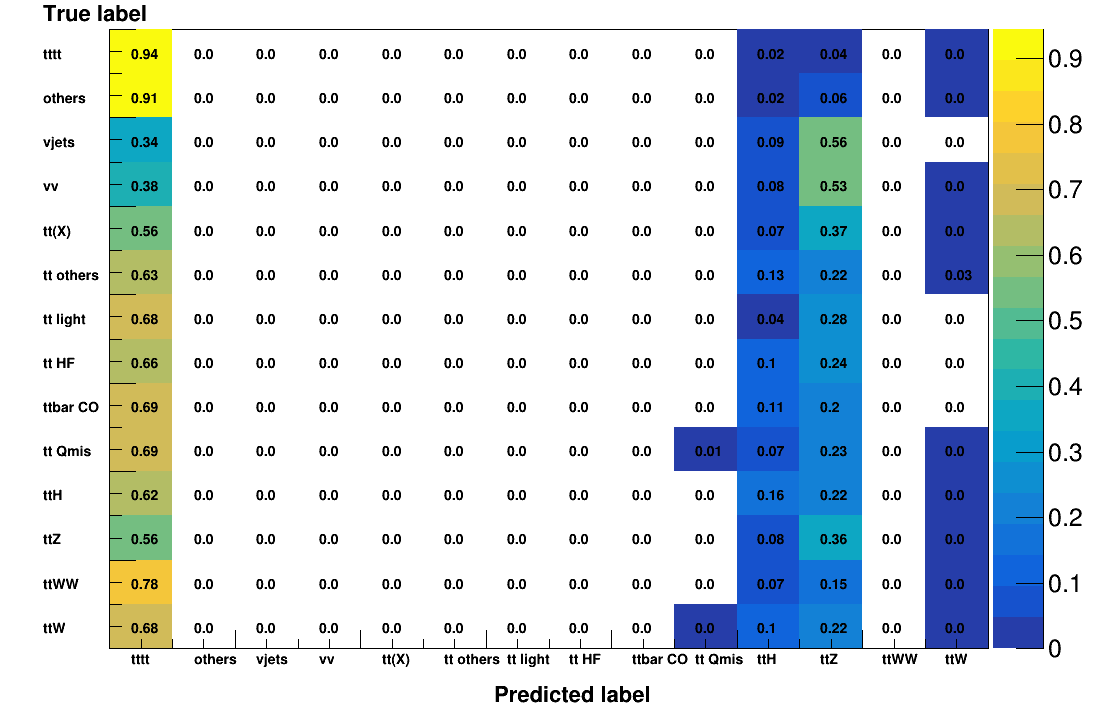
\includegraphics[width=.99\linewidth]{figs/MultiClass/Cm_unweighted}
  \caption{}
  \label{fig:CMunW}
\end{subfigure}%
\begin{subfigure}{.45\textwidth}
  \centering
  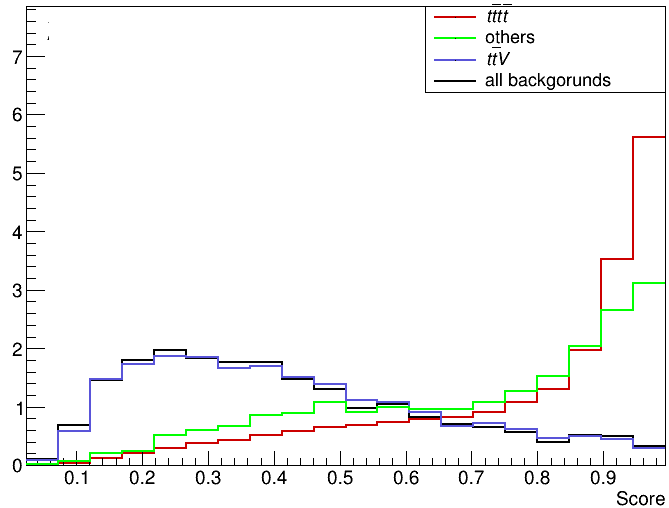
\includegraphics[width=.99\linewidth]{figs/MultiClass/Score_tttt_ttWothers}
  \caption{}
  \label{fig:Score14}
\end{subfigure}
\caption{The confusion matrix (a) and the Neural Network score (b) for the multi classification with 14 classes.}
\label{fig:14Class}
\end{figure}

The first multi classifier approach treats every background process as an individual class. Presenting the Neural Network with the opportunity to optimize the selection for each background. The best obtained $\Gamma_{\text{total}}$ is 0.852 and it did not increase the performance compared to the binary classification used previously. \\
Figure \ref{fig:Score14} shows the score for the most important backgrounds. The similarity between the $t\bar{t}t\bar{t}$ (red) and the $t\bar{t}t$ (green) observed in Section \ref{sec:FNN_results} is apparent since the highest fraction of events for both processes end up in highest bins. The dominant backgrounds $t\bar{t}V$ (blue) are most commonly assigned a score below 0.5 but also have considerable contributions up to scores of 0.8. All other backgrounds (black) have a similar distribution to $t\bar{t}V$. \\
In Figure \ref{fig:CMunW} the confusion matrix of the obtained classification is shown. The y-axis gives the information about the true event class. The predicated labels on the x-axis are determined by assigning an event to the class for which it has the highest probability. The numbers given in the different cells correspond to fractions of total events in the same row or column. A perfect classification would only have entries of 1 on the diagonal. The trained classifier has almost exclusively entries for three classes, which correspond to the processes with the highest yields. The $t\bar{t}t\bar{t}$ yield was renormalized to the combined total background yield as discussed in Section \ref{sec:transformation}. Therefore, it is beneficial for the Neural Network to focus on the correct identification of  $t\bar{t}t\bar{t}$ events rather than rejecting background events.

\newpage

\paragraph{Class Weights} \mbox{} \\

\begin{figure}[H]
\centering
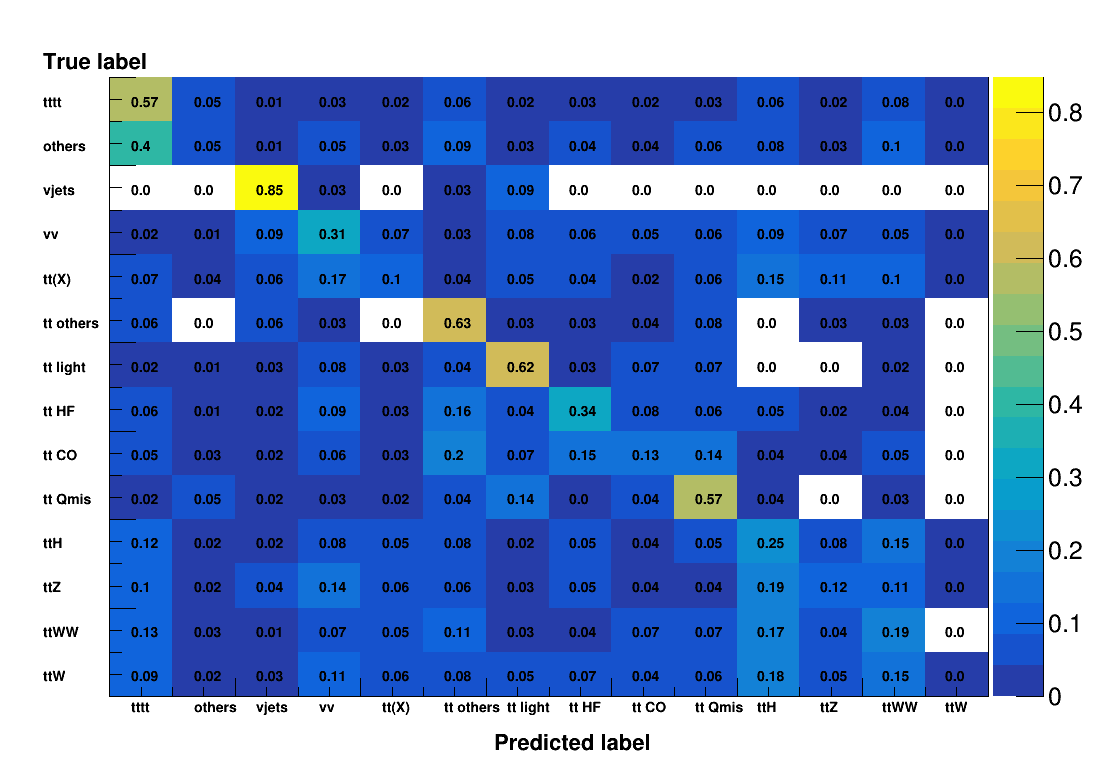
\includegraphics[width=\linewidth]{figs/MultiClass/Cm_classweights}
\caption{The confusion matrix for the multi classification with 14 classes where an additional class weight was applied during the training of the Classifier.}
\label{fig:CMWed}
\end{figure}

A way to force the neural network to pay more ``attention'' to minor backgrounds is to scale all processes to the same yield using class weights. This reweighting will decrease the AUC of the obtained classification. However insights about which backgrounds are most difficult to distinguish for $t\bar{t}t\bar{t}$ can be gained. Thus, providing a possibility to validate the observations about $t\bar{t}t$ (others). The class weights $w_{c}$ are calculated according to
\begin{equation}
w_{c} = \frac{N_{\text{total}} }{M \cdot N_{c}}
\end{equation}
where $N_{\text{total}}$ is sum of all yields and $N_{c}$ is the yield of class $c$. \\
The confusion matrix obtained by applying class weights is shown in Figure \ref{fig:CMWed}. As intended, most classes have their largest fraction of events on the diagonal. The separation between different classes is limited by the choice of the input variables that were selected to discriminate signal from all backgrounds and not to discriminate between different backgrounds individually. In agreement with the previous studies, the dataset ``others'' is the background with the highest fraction of events predicted to be signal events (0.4). The other signal like backgrounds for this classification are $t\bar{t}H$ and $t\bar{t}WW$.

\newpage

\paragraph{Three Classes} \mbox{} \\

In this approach, only three different classes are considered, namely a signal class, a class containing the most dominant backgrounds $t\bar{t}V$, and a class for all other backgrounds called ``rest''. No additional class reweighting is applied. This study aims to improve the AUC compared to the result obtained in the binary approach. The additional class of $t\bar{t}V$ is meant to help further reduce the dominant background.

\begin{figure}[H]
\begin{subfigure}{.55\textwidth}
  \centering
  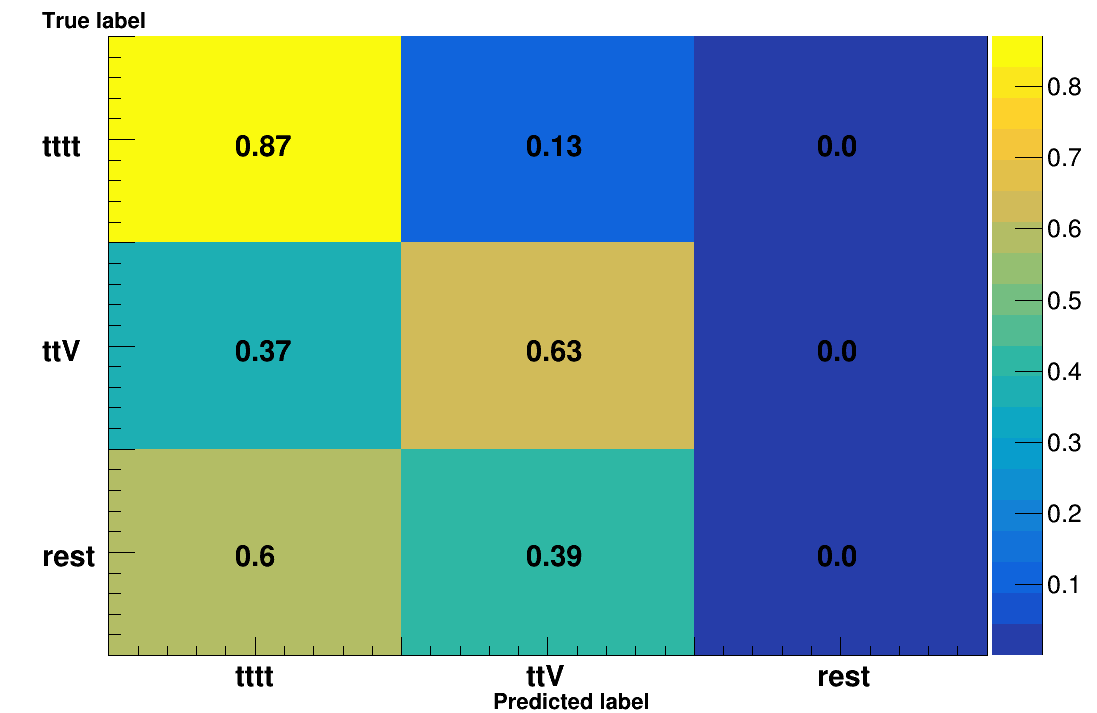
\includegraphics[width=.99\linewidth]{figs/MultiClass/CmOther}
  \caption{}
  \label{fig:CM3}
\end{subfigure}%
\begin{subfigure}{.45\textwidth}
  \centering
  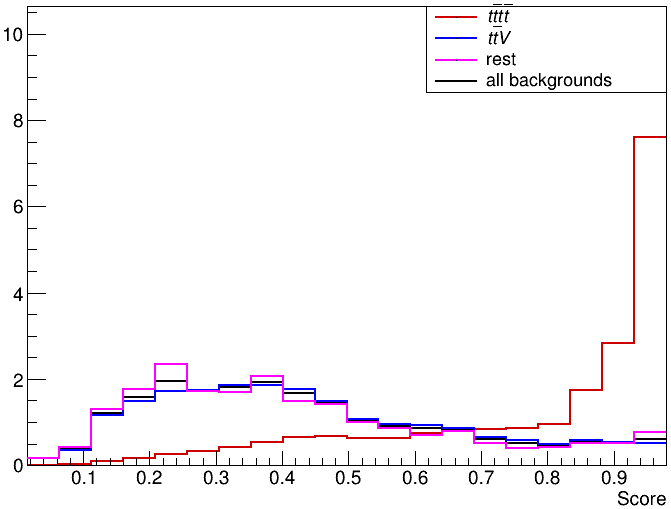
\includegraphics[width=.99\linewidth]{figs/MultiClass/ScoreFNN14Even_0}
  \caption{}
  \label{fig:Score3}
\end{subfigure}
\caption{The confusion matrix (a) and the Neural Network score (b) for the multi classification with 3 classes.}
\label{fig:3Class}
\end{figure}

The results of this approach is shown in Figure \ref{fig:3Class}. The events belonging to the ``rest'' class are identified as a signal or $t\bar{t}V$ event. This is because this class has a low combined yield of $\sim 86$ whereas $t\bar{t}V$ has a yield of 151 and $t\bar{t}t\bar{t}$ a yield of 237, during training. The identification of $t\bar{t}V$ has significantly improved compared to the previous multi classifier approaches. On the other hand, the identification of $t\bar{t}t\bar{t}$ has decreased from 0.94 (cf. Figure \ref{fig:14Class}) to 0.87. \\
The observed AUC for the classification with three classes is 0.854. This result seems to be contradict to the result of the binary classification approach with a AUC 0.853 where in the high score region (cf. \ref{fig:HTFNN}) better rejections of $t\bar{t}V$ and all the remainder backgrounds than 0.37 and 0.6 were found. However, the confusion matrix in Figure \ref{fig:CM3} assigns the event to the most likely category. Reviewing the background events ending up in the $t\bar{t}t\bar{t}$ category showed that most of them had scores below 0.8 but higher scores for $t\bar{t}t\bar{t}$ than for the other two categories.

\newpage


\section{Signal Classification using Recurrent Neural Networks}
\label{sec:RNN_results}

Compared to Feedforward Neural Networks, Recurrent Neural Networks are more complicated to train and more computationally expensive. A single neuron of the used LSTM neuron structure has 5 activation functions, each of which has specific functionalities that control the different cell states. Therefore, they different choices for this activation functions will not be considered. \\
The strategy chosen to study RNNs is restricted to the most impactful parameters, namely the number of parameters, the number of hidden layers, and the learning rate. The optimization algorithm selected is SGD and it is used in combination with polynomial learning rate decay to ensure that the training converge if a minimum is found in the parameter space. The maximum number of Epochs is restricted to 80, while the AUC is computed at every Epoch. The mean and the standard deviation needed to transform the input features are obtained based on all objects in the considered feature. To be more concrete, to transform the leading electron's pseudorapidity into a normal distribution, the $\eta$ of all electrons is considered during the calculation of mean and standard deviation. Only the 7 objects with the highest $p_{\text{T}}$ for each particle type and event are considered to avoid using variables with significant mismodeling. Since several of the $ 7 \cdot 13 = 84$ input features contain many zeros (due to zero padding), Lasso regression must be applied. The scaling constant $\alpha_1$ is fixed to 0.002.


\paragraph{Architecture} \mbox{} \\

\begin{figure}[H]
\centering
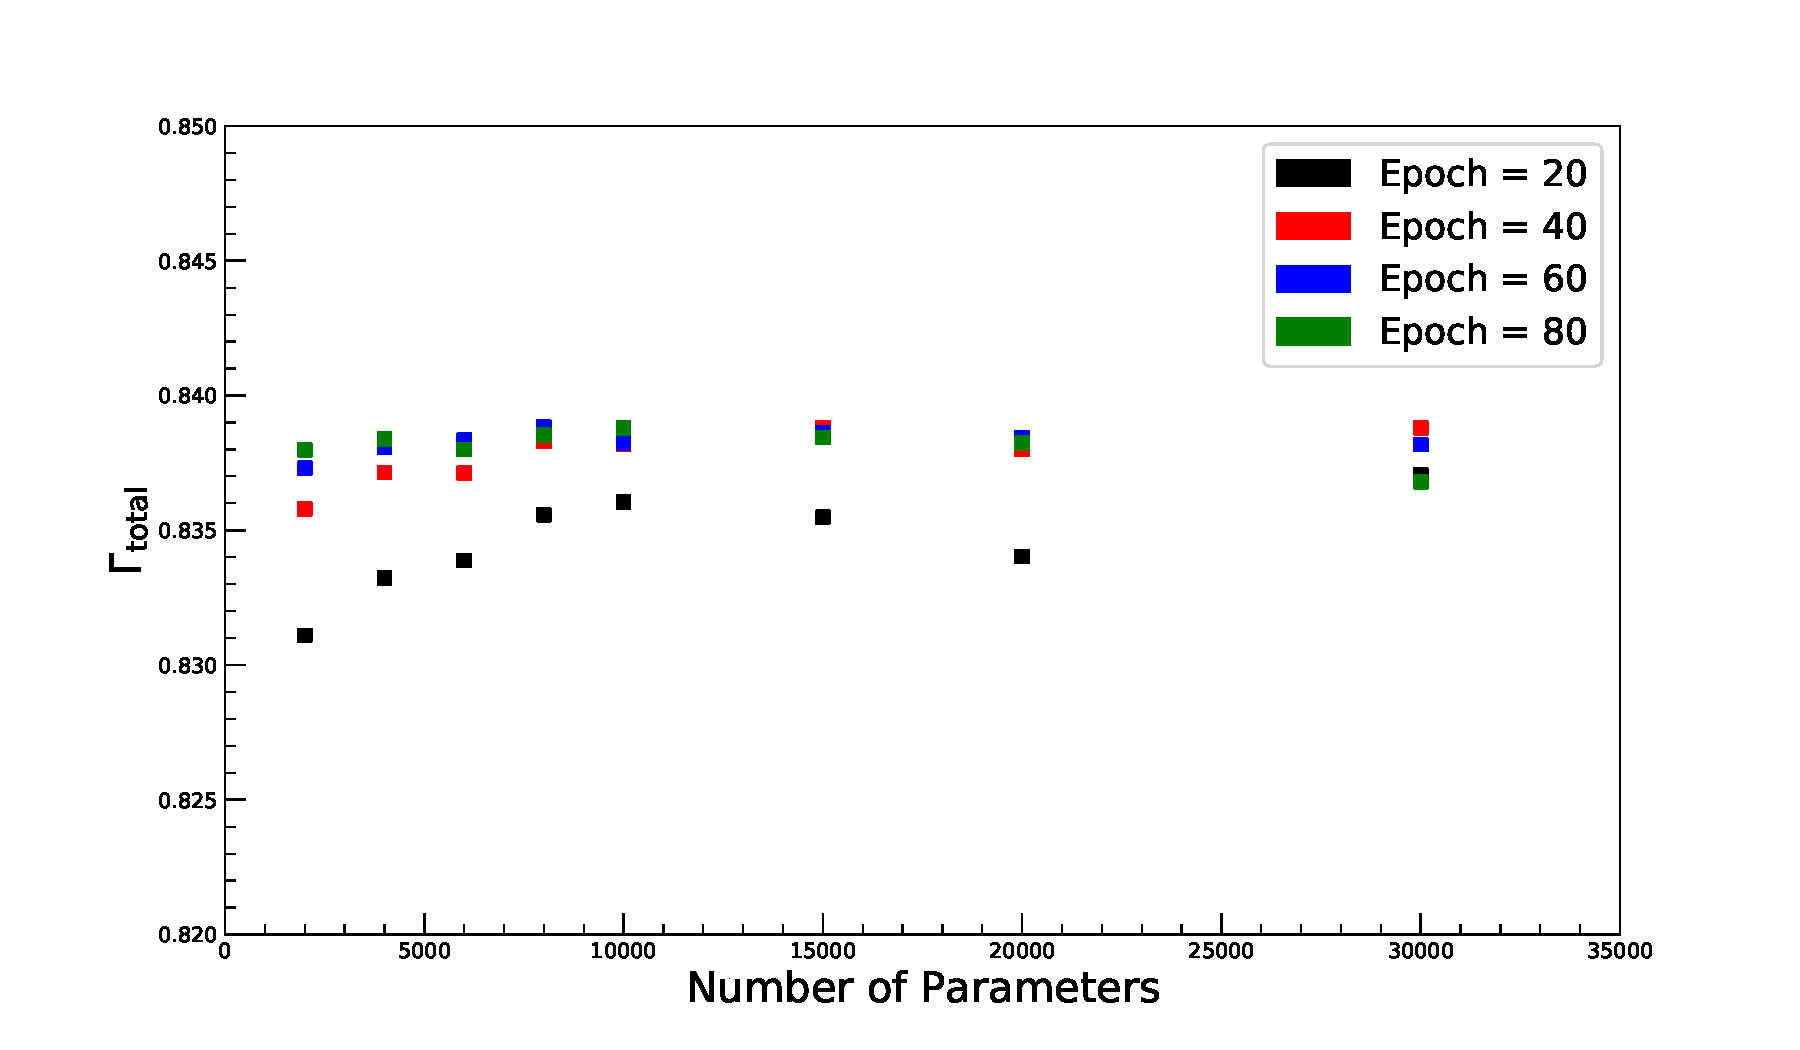
\includegraphics[width=\linewidth]{figs/RNN/AucPara_RNN}
\caption{The average overtraining for different RNNs configurations. The training is stopped after 20, 40, 60 and after 80 Epochs. The average includes the overtrainings of the 4 best-performing Neural Networks of different depth.}
\label{fig:ParaRNN}
\end{figure}


As for the FNNs, the number of parameters and the number of layers is investigated first. Based on the knowledge gained in the first architecture study (Section \ref{sec:FNN_results}), the range for the number of parameters considered is between 2000 and 30000. The number of hidden layers tested is restricted to a maximum of 4 hidden layers. \\
Figure \ref{fig:ParaRNN} shows the AUCs of Neural Networks with varying number of trainable parameters obtained at 20 (black), 40 (red), 60 (blue), and 80 (green) Epochs. Every quoted $\Gamma_{\text{total}}$ is average over the 4 different hidden layer configurations considered. The performance for 40, 60, and 80 Epochs is similar for the most studied sizes, while the training at 20 Epochs has not converged yet. The Neural Networks with 30000 parameters evaluated at Epoch 80 show a decrease in performance, which hints to the fact that these models started to overtrain. \\
Almost all models have an overtraining below 3\%, implying that the applied regularization is sufficient. The overtraining is independent of the number of parameters and hidden layers in the Neural Networks, which indicates that all trainings converged. \\
The Neural Networks with 1 or 2 hidden layers outperformed Neural Networks with 3 or 4 hidden layers in all cases considered. The peak performance of $\Gamma_{\text{total}} = 0.838$ is reached by a Neural Network with 15000 parameters and two hidden layers.

\paragraph{Learning Rate and Batch size} \mbox{} \\

\begin{figure}[H]
\centering
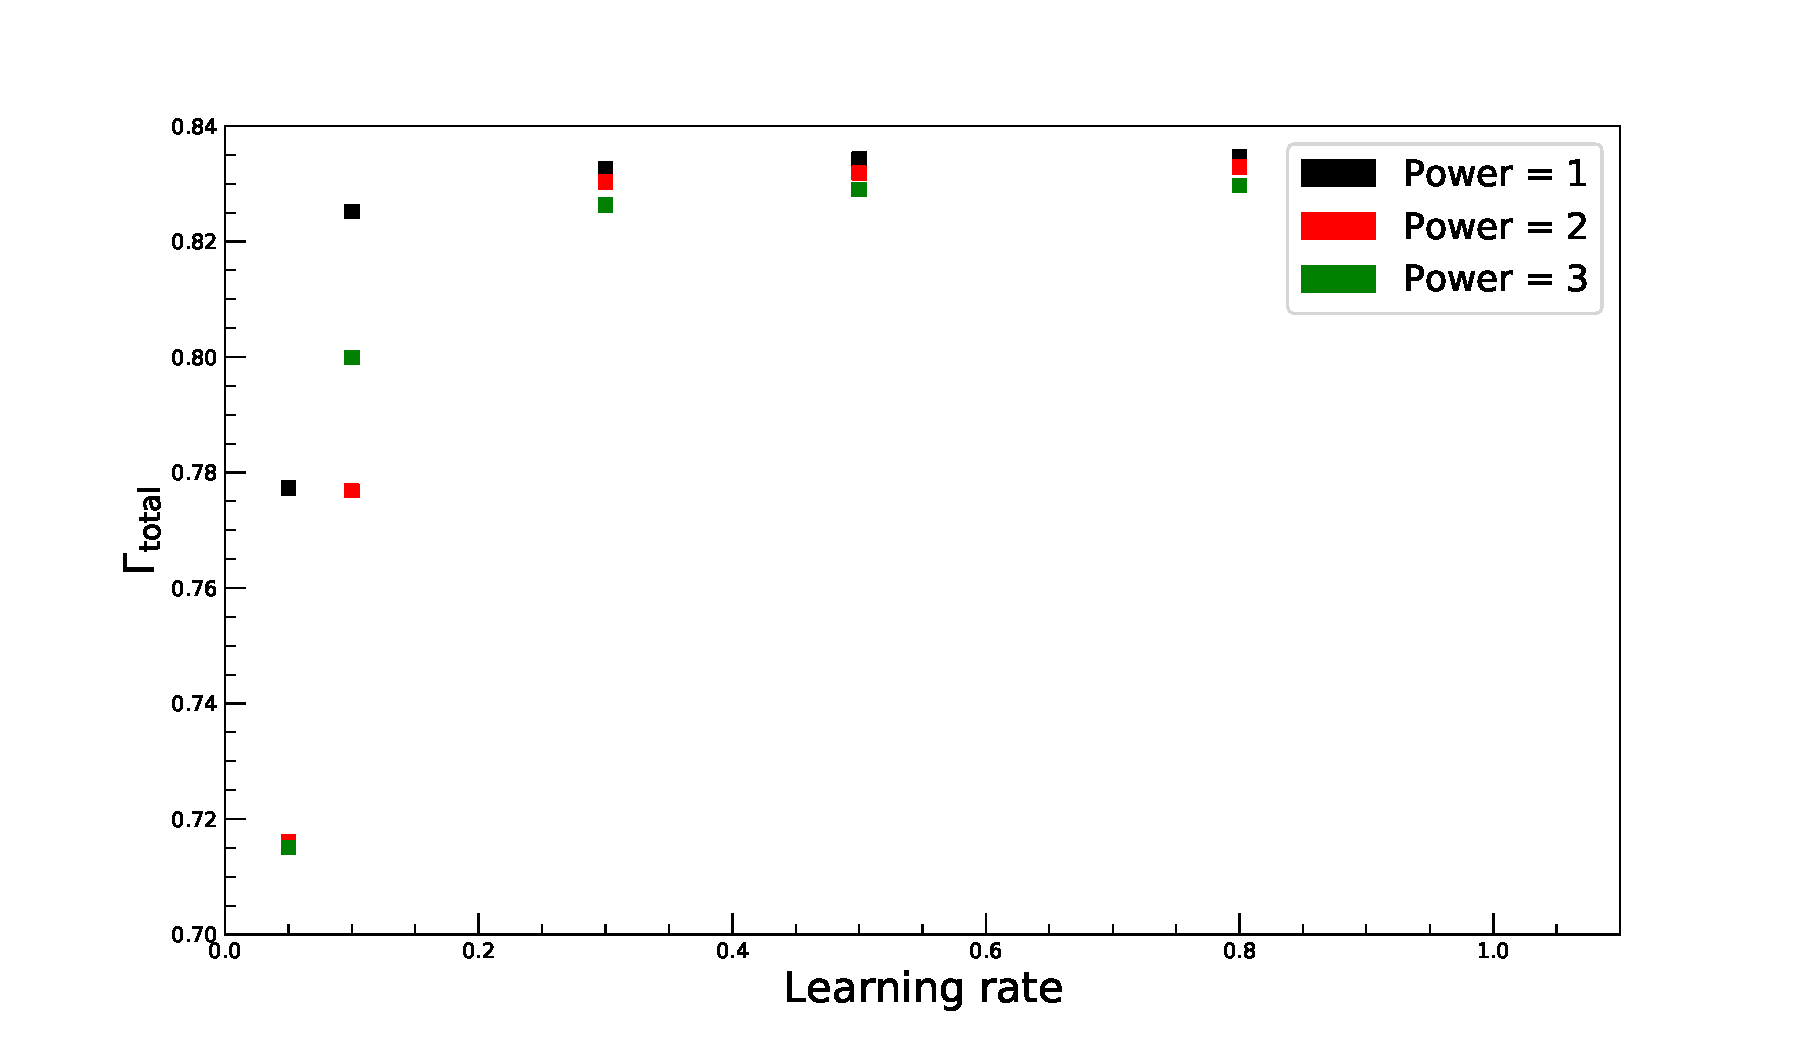
\includegraphics[width=\linewidth]{figs/RNN/LrAuc_Fixed}
\caption{The obtained average AUC of RNNs with different learning rates. The average includes the AUCs of the 2 best-performing Neural Networks with different batchsizes.}
\label{fig:LrRNN}
\end{figure}

The Neural Network with the best performance in the previous study is selected to investigate the AUCs dependence on the learning rate and the batch size. The considered batch size reaches from $10^{11}$ to $10^{14}$, which was observed to be a high-performance region for FNNs. Following the same logic, learning rates between 0.05 and 0.8 with decay polynomials of power 1 to 3 are selected. \\
Figure \ref{fig:LrRNN} shows the average AUCs obtained using the different learning rates and decay polynomials. The average includes the results for the two best performing considered batch sizes (2048 and 4096). Similar to the observed results for FNNs, the performance of RNNs is stable within one order of magnitude around the learning rate that performs the best. Outside of the stable region, it decreases the performance of RNNs rapidly. Similarly, the power of the chosen polynomial has a minor influence on the performance inside the stable region, whereas outside of the region, it can have a significant influence.  One reason for this could be the more complex and thus more fragile training procedures for RNNs compared to FNNs. On the other hand, the fact that the learning rate decay of order 1 worked the best implies that the Neural Networks might not have converged. The Epoch at which the highest AUC is reached is close to the maximum 80 Epochs but more than 5 Epoch away. Therefore, a combination of both effects is the most likely explanation for the rapid drop. \\

\begin{figure}[H]
\centering
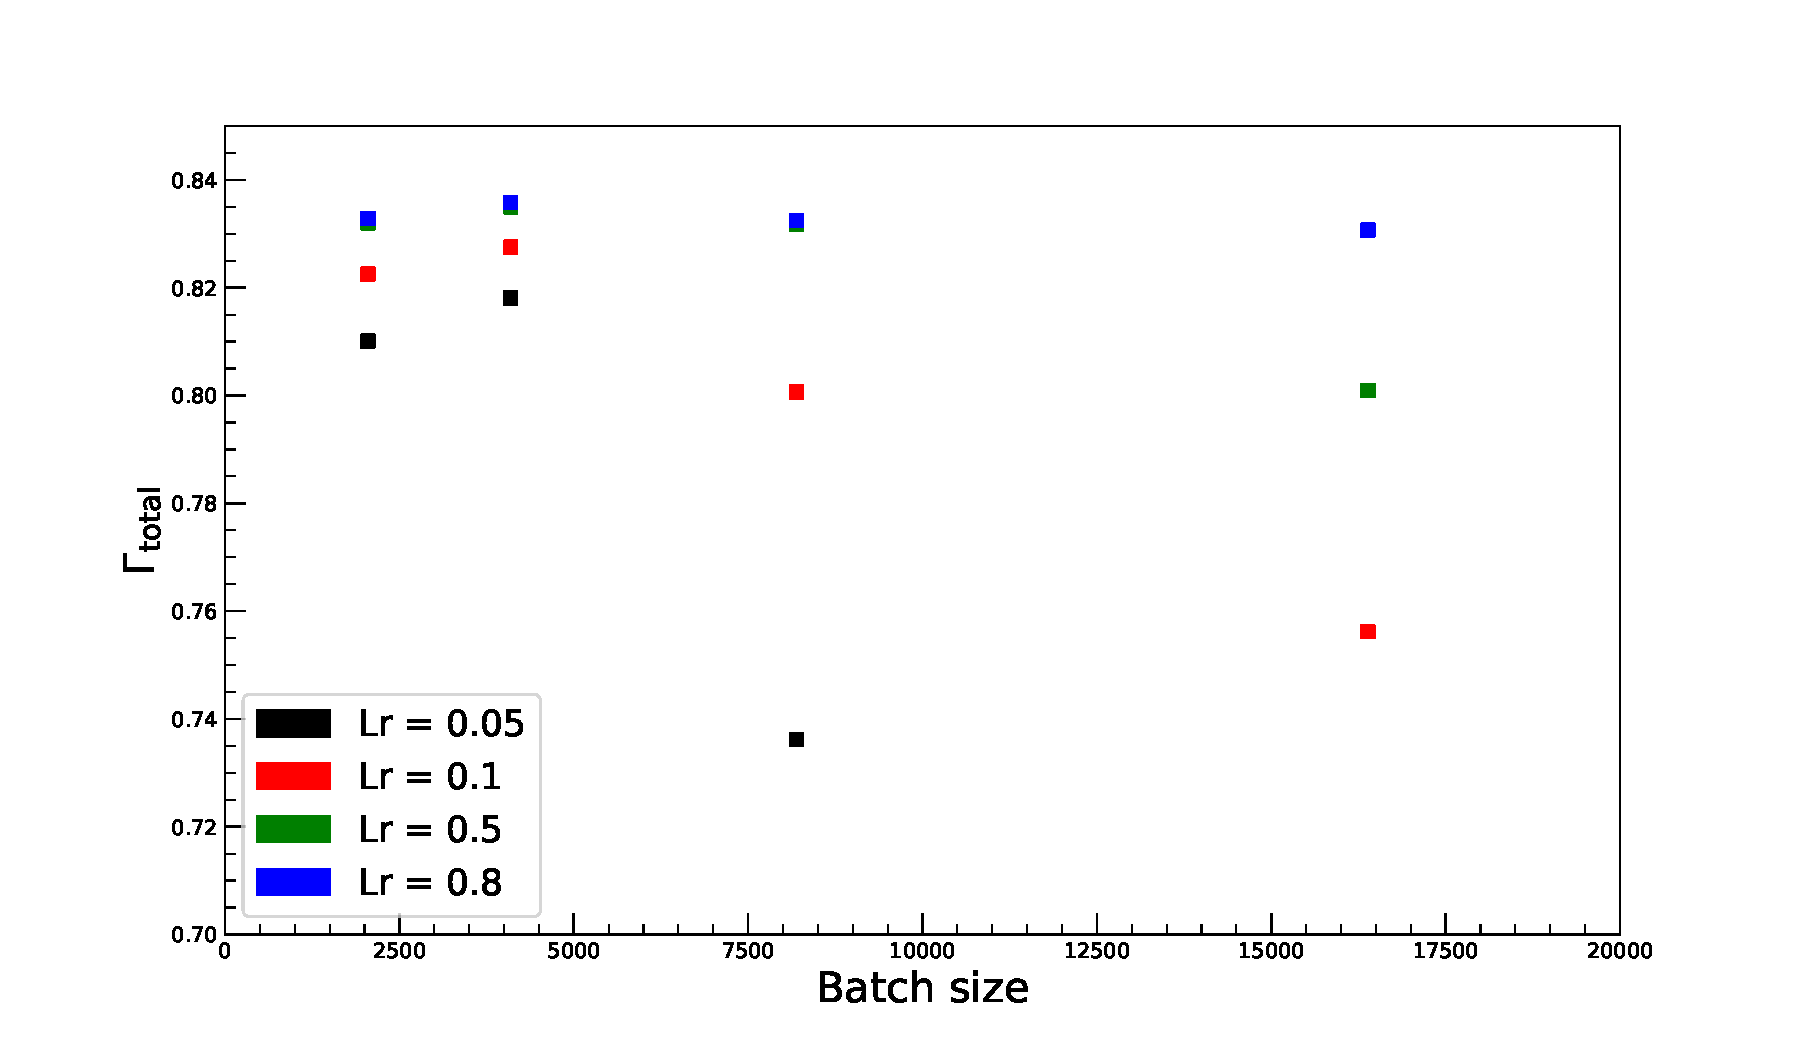
\includegraphics[width=\linewidth]{figs/RNN/BatchOv_Fixed}
\caption{The AUC as a function of the batch size and the learning rate.}
\label{fig:BatchRNN}
\end{figure}

The dependence of the AUC on the batch size is shown in Figure \ref{fig:BatchRNN}. A similar dependence as for the FNNs can be observed. For learning rates close to the optimal value obtained, the batch size has a minor influence on the performance of the Neural Networks. For smaller learning rates, the dependence is larger. The decrease in performance when choosing a large batch size, when combined with a small learning rate, is larger than the observed decrease for FNNs. This validates the assumption that the more complex training of RNNs is sensitive to the choice of hyperparameters. \\
The best performing RNN has a significantly smaller AUC (0.842) than the best performance observed using FNNs (0.854). Therefore, the initial idea to present the Neural Network with the possibility of using the full information available did not improve $\Gamma_{\text{total}}$. The RNN failed in combining the input features in a way that discriminates the signal from the background more than the features used for FNNs, which are constructed using physical knowledge. \\
The overtraining of all considered Neural Networks is below 3\%. Figures showing the dependence of overtraining on the batch size and the learning rate can be found in Appendix \ref{ap:addRNN}.

\newpage

\paragraph{Achieved Separation} \mbox{} \\

\begin{figure}[H]
\centering
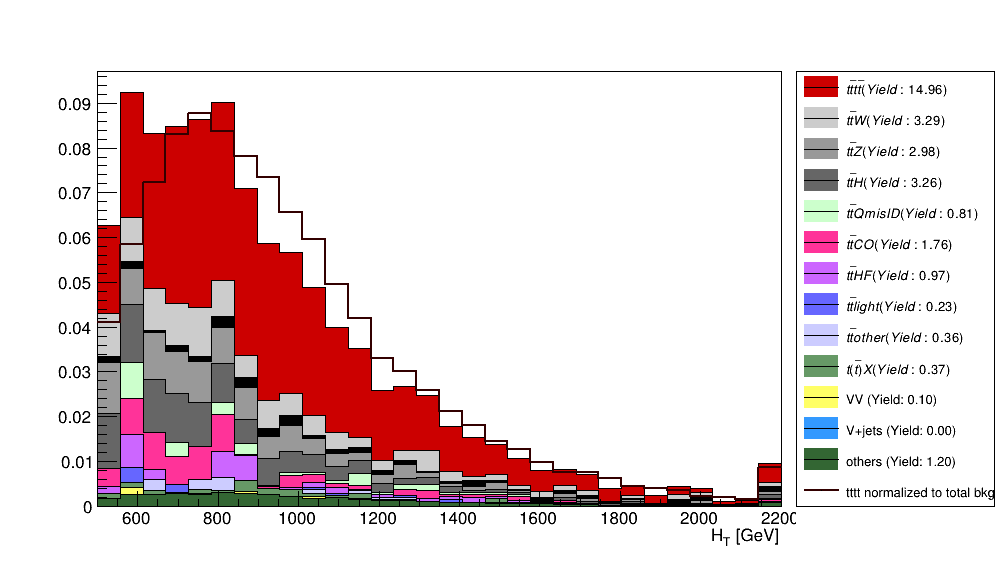
\includegraphics[width=\linewidth]{figs/RNN/HT_all_Even}
\caption{The $H_{\text{T}}$ distribution after applying a cut (optimized on the signal efficiency) to the RNN score obtained for the training on the background dataset containing even event numbers. The last bin additionally contains all events with $H_{\text{T}} > 2200$.}
\label{fig:RNNHT}
\end{figure}


Proceeding in the same way as for the FNNs, a cut based on the signal efficiency is optimized on the RNN score. Events passing that cut contribute to the $H_{\text{T}}$ distribution shown in Figure \ref{fig:RNNHT}. The selected RNN is the best-performing Neural Network from the learning rate and batch size study in the previous sub-section. It was trained on the background dataset, which contains events with odd event numbers. The score of the RNN can be found in the Appendix \ref{ap:addRNN} together with both the score and the $H_{\text{T}}$ distribution of the corresponding RNN trained on background events with odd event numbers. \\
The optimized cut is determined to be 0.85. The signal efficiency in the signal region improves from 1.8 to 2.7. As expected, is this signal efficiency lower than the one observed for the best FNN (2.9). The comparison between the background yields after applying the respective cuts to the FNN and RNN scores is shown in table \ref{tab:Rejcomb} where $\kappa$ and $\zeta$ are functions of the signal efficiencies $s$ and are calculated according to
\begin{equation}
\kappa = s \cdot Y'_{\text{sig}} 
\label{eq:kappa}
\end{equation}
\begin{equation}
\zeta = \frac{\kappa_{\text{FNN}} - \kappa_{\text{RNN}}}{Y_{\text{sig}}}
\label{eq:zeta}
\end{equation}
where $Y'_{\text{sig}}$ is the signal yield after applying the cut and $Y_{\text{sig}}$ before. As can be seen, the reduction measure $\kappa$ of all backgrounds is higher for FNN than for RNNs. The background hardest to reduces is $t\bar{t}t$. The dominate background $t\bar{t}W$, $t\bar{t}Z$ and $t\bar{t}H$ are reduced the most. $\zeta$ was designed with the intend to investigate from which backgrounds the performance decrease of the RNN, compared to the FNN, originates from. The backgrounds $VV$ and $t(\bar{t})X$ have the highest $\zeta$ values which indicates that these background especially benefit from the engineered features in the FNN. 

\begin{table}[H]
\begin{tabular}{|r|r|r|r|r|r|r|r|r|r|r|r|}
\toprule
measure & $t\bar{t}W$ & $t\bar{t}Z$ & $t\bar{t}H$ & $t\bar{t}$QmisID & $t\bar{t}$CO & $t\bar{t}$HF & $t\bar{t}$light & $t\bar{t}$other & $t(\bar{t})X$ & $VV$ & others \\
\midrule
\midrule
$\kappa_{\text{FNN}}$ & 33.8 & 33.6 & 33.7 & 53.1 & 45.5 & 68.9 & 111.3 & 74.7 & 100.8 & 197.7 & 59.4 \\
$\kappa_{\text{FNN}}$ & 29.4 & 29.2 & 29.3 & 46.2 & 39.6 & 60.0 & 96.9 & 65.0 & 87.7 & 172.0 & 51.7 \\
$\zeta$ & 0.07 & 0.09 & 0.11 & 0.51 & 0.27 & 0.56 & 2.15 & 1.54 & 2.55 & 5.84 & 2.52 \\
\bottomrule
\end{tabular}
\caption{The reduction measure $\kappa$ (defined in Equation \ref{eq:kappa}) for the high FNN and RNN region and there scaled difference $\zeta$ (defined in Equation \ref{eq:zeta}).}
\label{tab:Rejcomb}
\end{table}

\paragraph{Validation and Error Estimation} \mbox{} \\

\begin{figure}[H]
\centering
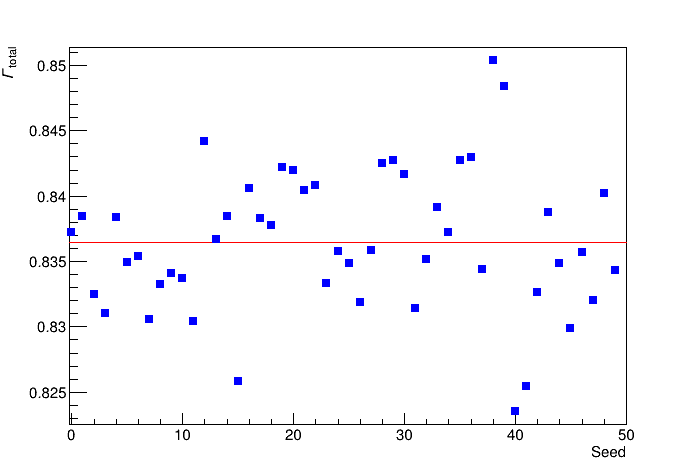
\includegraphics[width=\linewidth]{figs/RNN/BootStrap_RNN}
\caption{AUCs observed by using the bootstrap method on the validation set. The seed quoted (times 365) is the random seed used to generate the different resampled versions of the validation set. The red line indicates the mean of all observed AUCs.}
\label{fig:RNNBootStrap}
\end{figure}

The obtained AUC on the testing dataset (0.842) needs to be validated to 
ensure that no additional bias during the hyperparameter tuning was introduced. As for the FNN, the validation realized by obtaining the AUC on the resampled versions of the validation sample. Figure \ref{fig:RNNBootStrap} shows the observed AUCs and there mean value (red line) $\Gamma = 0.838$. The standard deviation represents the error of the obtained result and was determinate to be 0.006. Therefore, is the observed performance on the testing set within the exacted error.


\newpage

\section{Performance Evaluation of CPUs and GPUs}
\label{sec:CPUGPU}

All Neural Networks used in the previous studies were trained on Central Processing Units (CPUs). However, in deep learning applications, it is prevalent to use Graphics Processing Units (GPUs). \\
Most operations performed during a Neural Network training are simple matrix multiplication of weight matrices and feature matrices. CPUs are designed to perform few but complicated tasks and struggle with multiple threads at the same time. On the other hand, GPUs are designed to perform simple but many tasks at the same time, making them the optimal choice for deep learning applications. \\
The following study investigates the training time of Feedforward Neural Networks and Recurrent Neural Networks using CPUs and GPUs.
The same datasets that were used in the previous Neural Network studies are utilized in here. The devices used for the training are Intel Xeon e5-2620 v3 CPUs and Geforce gtx 1080 GPUs. \\
Neural Networks with sizes between 2000 and 70000 parameters are considered. The optimization algorithm used is SGD, with batch sizes between $2^{10}$ and $2^{16}$. All other parameters are fixed to the best-performing Neural Networks of each type. The AUC evaluation at each Epoch is turned off since the needed calculations can take several seconds. The reported train time per Epoch is the average over 120 Epochs. \\

\begin{figure}[H]
\centering
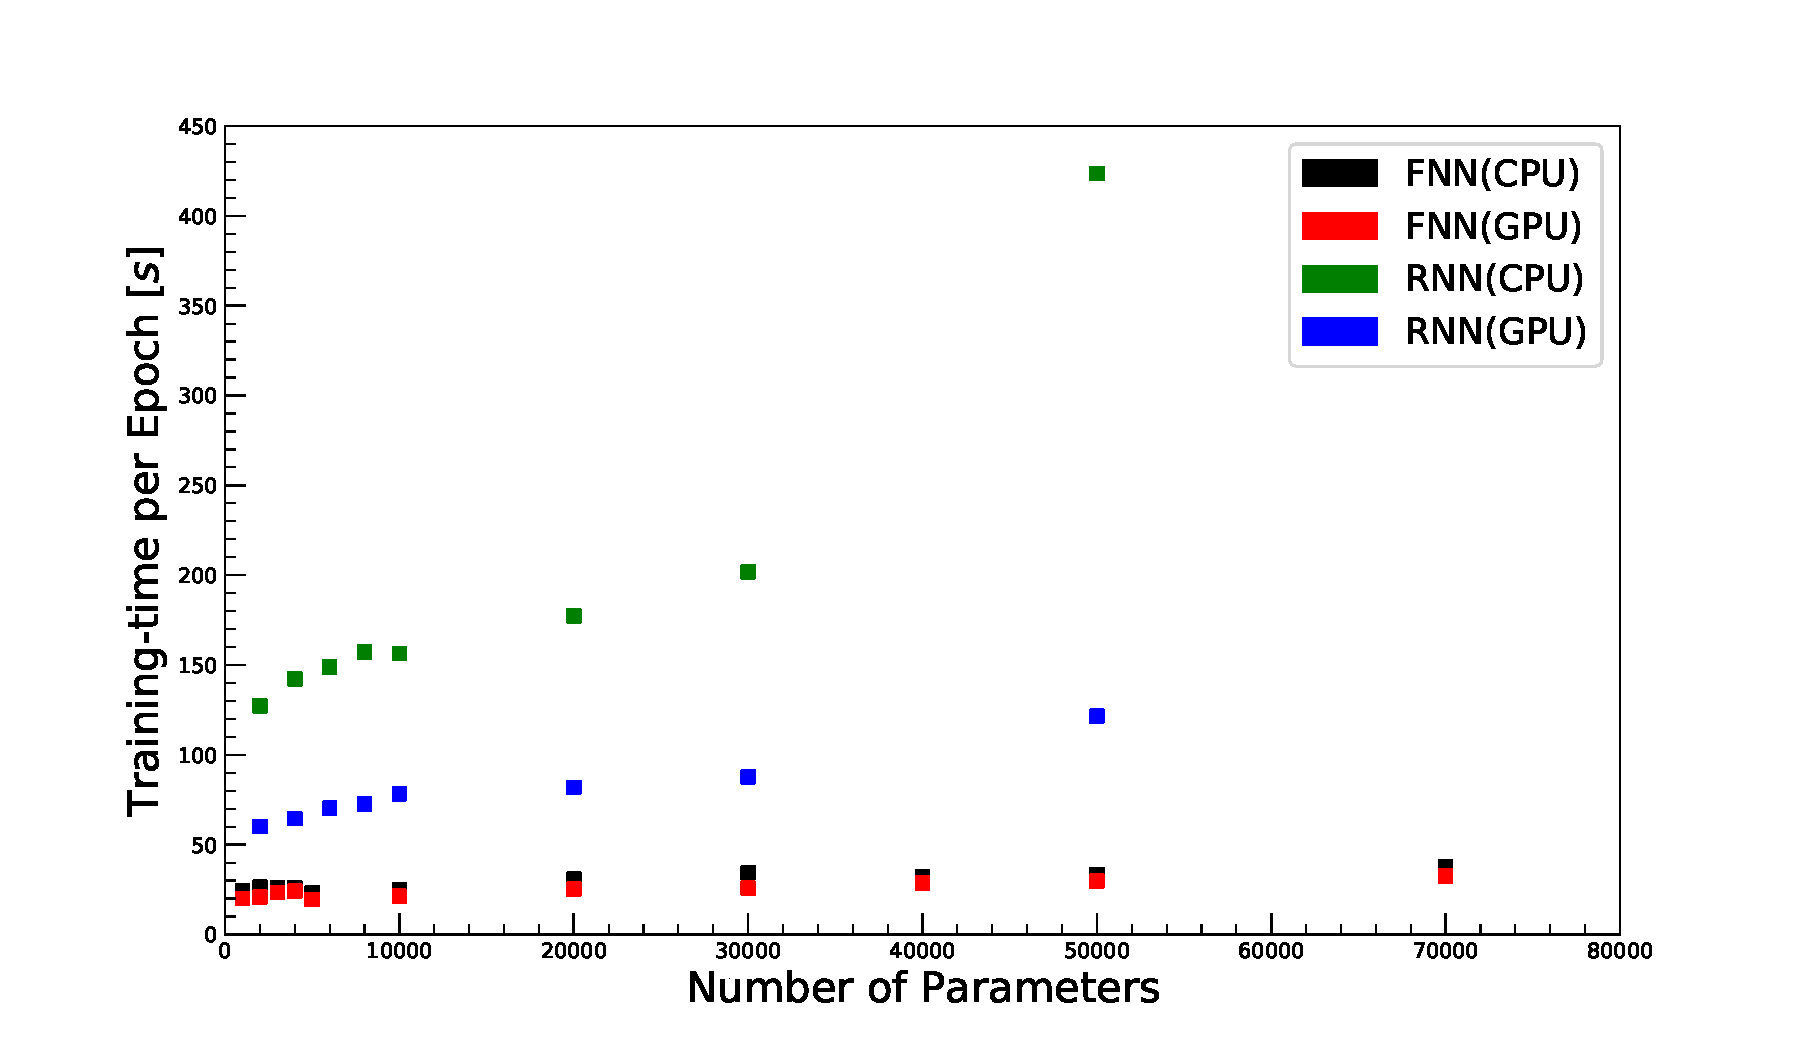
\includegraphics[width=\linewidth]{figs/CPUGPU/NumParaTraintime_Fixed}
\caption{Training times per Epoch for FNNs and RNNs of different sizes trained on CPUs and GPUs.}
\label{fig:CPUGPUPara}
\end{figure}

Figure \ref{fig:CPUGPUPara} shows training time for the Neural Networks of different sizes where the batch size was fixed to 8192. The RNNs take significantly longer to train than the FNNs due to their more complicated neuron structure and training algorithm. GPUs outperform CPUs for all considered Neural Networks. The gain in performance is especially high for Neural Networks with many tunable parameters. For the largest RNNs training time decreases per Epoch by a factor of 4 when using GPUs compared to CPUs. \\
The results for the different batch sizes are shown in Figure \ref{fig:CPUGPUBatch}, where a Neural Network with 50000 parameters was used. Again GPUs outperform CPUs over the full parameter space selected. The decrease in training time is small for small batch size and increases with larger batch sizes. The reason for this is that only the calculations within one iteration are performed simultaneously. Since the number of performed calculations scale with the batch size, also the performance gain does. The saturation of performance gain for Neural Networks with batch size larger than $\sim16000$ most likely has two sources. The first one being that for this batch sizes the matrices get so large that the GPUs reach their limit in terms of maximum number of calculations that can be performed at the same time. The second possible explanation is the observed standard deviation of the training times per Epoch was significantly higher for the batches of $2^{15}$ and $2^{16}$. This indicates that the cluster node started to lag, potentially influencing the obtained result. \\
In conclusion it can be stated that even for the small datasets and Neural Networks considered, the usage of GPUs is highly advisable.

\begin{figure}[H]
\centering
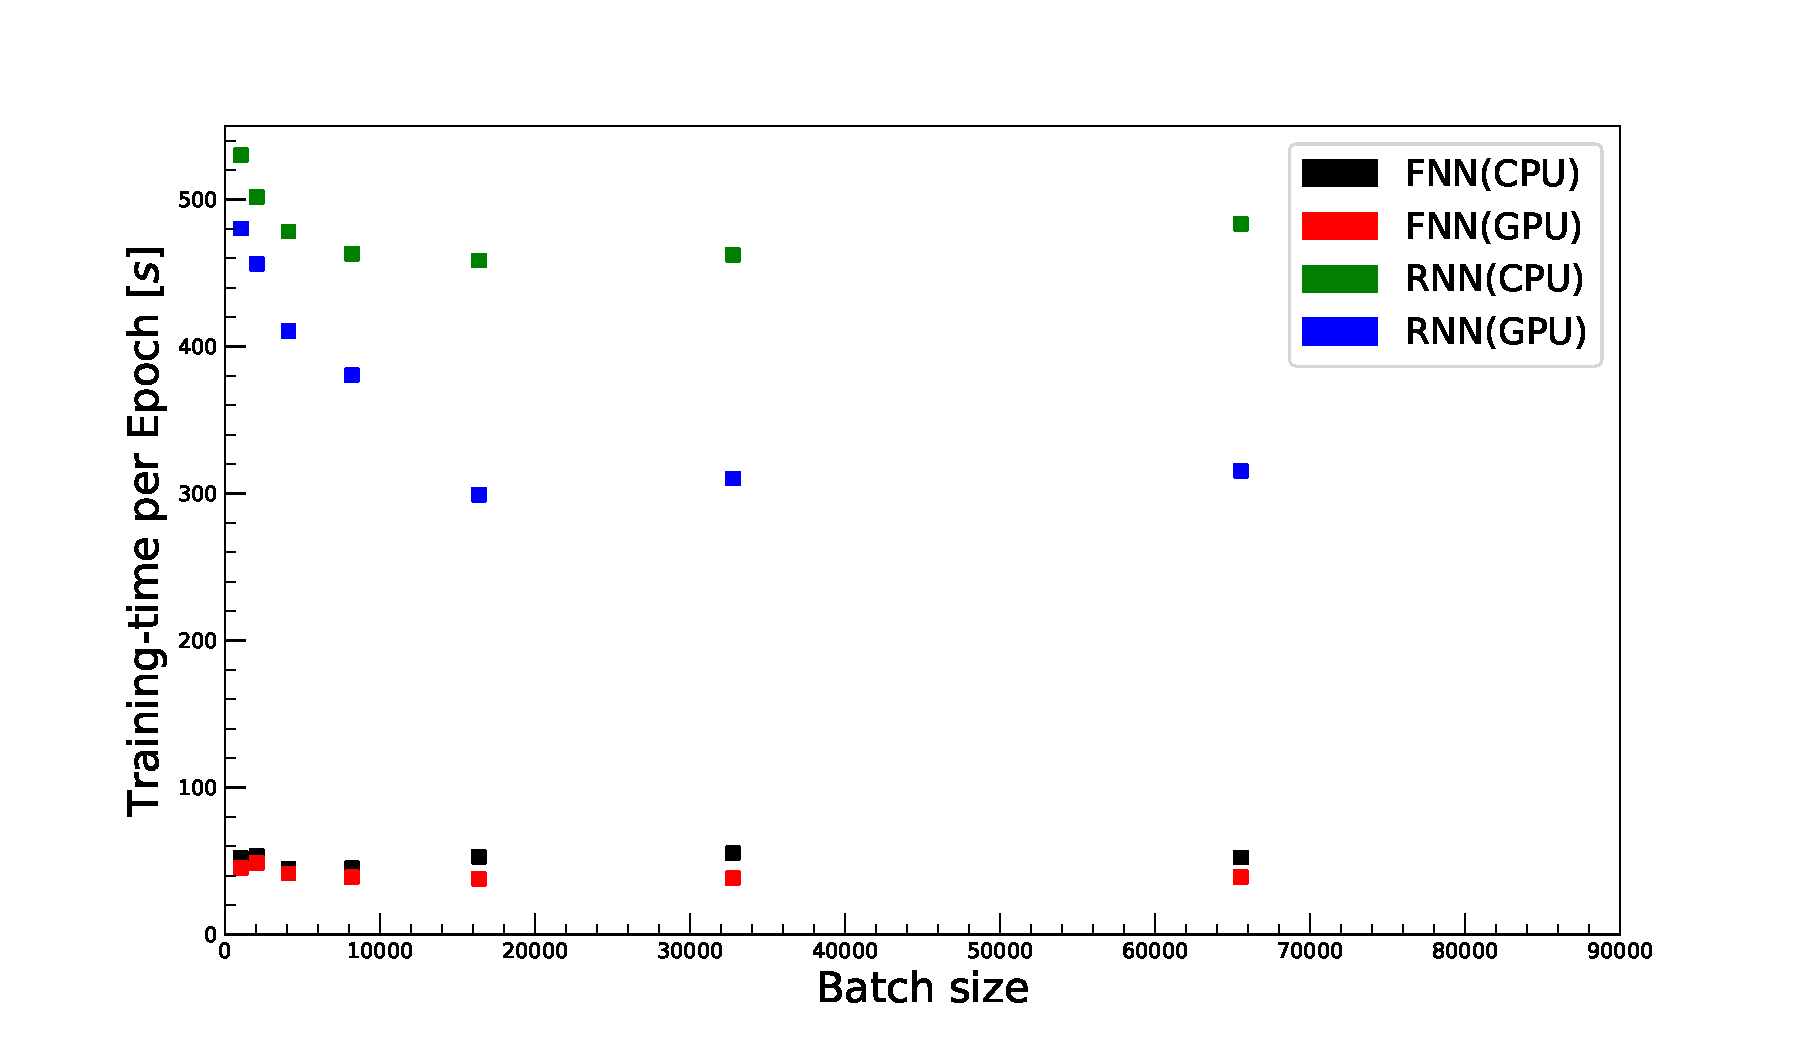
\includegraphics[width=\linewidth]{figs/CPUGPU/BatchTraintime_Fixed}
\caption{Training times per Epoch for FNNs and RNNs trained with different batch sizes and on CPUs and GPUs.}
\label{fig:CPUGPUBatch}
\end{figure}

\newpage

\section{Reconstruction of Two Hadronic Top Quarks}
\label{sec:TwoHadTop}

The $t\bar{t}t$ contamination in the high score regions of the FNN, the RNN, and the BDT used in the official $t\bar{t}t\bar{t}$ analysis motivate the search for a feature that discriminates the two processes well. Since both processes are very similar in their kinematics, the chosen approach aims at the final state particle composition. In the same-sign two lepton channel, two of the four $W$ bosons that originate from four top quark decays, decay
hadronically. On the other hand, a $t\bar{t}t$ event produced without any associated particles has one hadronically decaying W boson in the final state. As discussed in Section \ref{sec:Theory3top} such a production is not possible at leading order. In practice make the particles produced in association with the $t\bar{t}t$ the separation of $t\bar{t}t\bar{t}$ and $t\bar{t}t$ more complicated. Incorrect reconstruction of jets or leptons and charge misidentification can further disturb a possible reconstruction. \\
The datasets used for the reconstruction were introduced in Chapter \ref{sec:Samples}. The signal region is redefined to match the conditions of the two hadronic top quark reconstruction. Events with 3 or more leptons are rejected; only events with two leptons with charges have the same sign are considered. The number of required jets is raised from at least 6 jets to at least 8 jets. All other signal region conditions stay the same.

\paragraph{Reconstruction principle} \mbox{} \\

The reconstruction technique presented in the following tries to identify $t\bar{t}t$ events by final states that have one hadronic top quark and $t\bar{t}t\bar{t}$ events by final states that have two hadronic top quark. Priority is given to the reconstruction of two hadronic top quarks, which are reconstructed from 6 jet combinations, 3 jets for each top quark. At least one of the two top quark candidates has to contain a b-jet. The assignment of the three jets to a W boson and a b-jet depends on the number of b-tagged jets contained within the top quark. If only one of the jets is b-tagged, this jet is assigned to the b-jet, and the two other jets are said to be the decaying produces of the W boson. If two jets are b-tagged, the two jet combination with the lowest discriminator is selected, but at least one b-tagged jet has to be assigned to the b-jet. If non or all jets are b-tagged, the combination with the lowest discriminator is selected. \\  
The discriminator chosen for the reconstruction is based on $\chi^2$ and contains one term for each of the four reconstructed objects (2 top quarks and 2 W bosons). 
\begin{equation}
\label{eq:Chi2had}
\chi^2_{\text{2had}} = \chi^2_{t_1} + \chi^2_{t_2} + \chi^2_{W_1} + \chi^2_{W_2}
\end{equation}
The individual $\chi^2$ terms are defined as
\begin{equation}
\label{eq:Chi2}
\chi^2_X = \frac{(m_{3/2j} - m_X)^2}{\sigma_X^2}; \,\,\,\,\,\, X \in {t,W}
\end{equation}
where $m_{3/2j}$ is the mass of the 3 or 2 jet combination. The mass and the width of the top quark and the W boson are obtained from the dataset, which will be discussed in the next sub-section. \\
The reconstruction of two hadronic top quarks is defined to be successful if $\chi^2_{\text{2had}}$ does not exceed a critical value $\chi^2_{c1}$. The exact value of $\chi^2_{c1}$ is left as a tunable parameter of the reconstruction. If $\chi^2_{\text{2had}}$ is smaller than the $\chi^2_{c1}$, the reconstruction of one hadronic top quark is carried out. The reconstruction of one hadronic top quark proceeds in the same way as the two hadronic top quark reconstruction using the discriminator $\chi^2_{\text{1had}} = \chi^2_{t_1} + \chi^2_{W_1}$. If $\chi^2_{\text{1had}}$ surpasses a second critical value $\chi^2_{c2}$, the event is considered to have no hadronic top quark.

\newpage

\paragraph{Calibration} \mbox{} \\

\begin{figure}[H]
\begin{subfigure}{.5\textwidth}
  \centering
  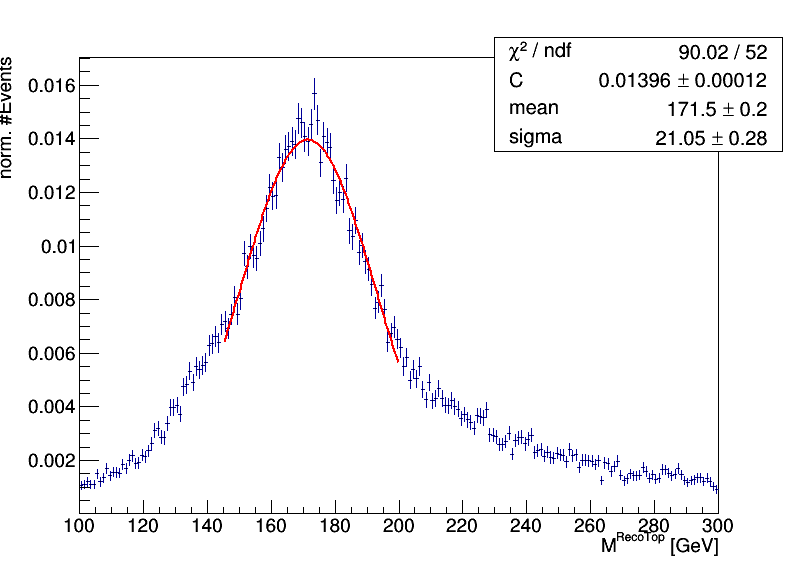
\includegraphics[width=.99\linewidth]{figs/HadTop/TopMass}
  \caption{Top Quark}
  \label{fig:Calt}
\end{subfigure}%
\begin{subfigure}{.5\textwidth}
  \centering
  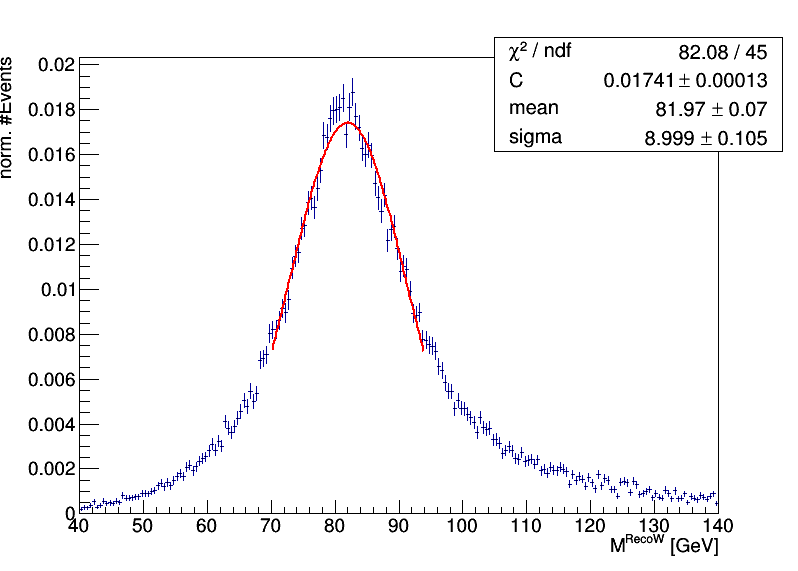
\includegraphics[width=.99\linewidth]{figs/HadTop/WMass}
  \caption{$W$ boson}
  \label{fig:CalW}
\end{subfigure}
\caption{Mass distributions of the truth matched and reconstructed top quarks (a) and W bosons (b).}
\label{fig:Cal}
\end{figure}

The calibration of the top quark and W boson mass and width is performed by matching the reconstruction candidate to the \textit{truth particles}. The kinematic and final state particles of the truth particles are known from the truth information in the used datasets. Only hadronically decaying truth top quarks or W bosons with final state particles that can be measured by the ATLAS detector are considered. The matching is performed based on the $\Delta R$ between the reconstruction candidates and the truth top quarks in the same event. The closest reconstruction candidate is assigned to the truth top quark. The matching of W bosons is performed in the same way and independently of the matching of top quarks. \\
Only matched pairs that have a $\delta R(\text{reco},\text{truth})$ smaller than the critical value are considered for the final mass fit. Figure \ref{fig:Cal} shows the result of the calibration with a critical value of $\delta R(\text{reco},\text{truth}) < 0.4$. The mass and the width of the particles is observed as the mean and standard deviation of the gaussian fit.  The obtained masses and width are $m_t = 172$, $m_W = 82$, $\sigma_t = 21$, and $\sigma = 9$. \\
To study the dependence of the observed masses and widths, different critical values between 0.1 and 0.8 were considered. The mean of the distribution is approximately independent of the critical value. The standard deviation varied between 22.6 and 16.9 for the top quark and between 7.7 and 9.6 for the W boson. The critical value of $\Delta R(\text{reco},\text{truth}) < 0.4$ was selected as the point at which both weight distributions showed an approximately symmetric peak. \\
In order to have a comparison to the results discussed in the next sub-section, a \textit{best-possible reconstruction} is defined. This reconstruction also uses truth information and, therefore, can not be used for measured data. All pre-requirement concerning the number of b-jets in the reconstructed particles are the same as for the $\chi^2$ based reconstruction. The best-possible reconstruction first selects all top quark candidates with a mass within $3\sigma$ around $m_t$ and contain a W candidate within $3\sigma$ around $m_W$. If there are more truth top quarks than reconstructed top quarks, the mass windows are broadened to $4\sigma$. If the number of truth top quarks still exceeds the number of reconstructed top quarks, all candidates are kept. After this pre-selection is finished, the matching based on $\delta R(\text{reco},\text{truth})$ as described previously is performed. The candidates closest to the truth top quarks in the same event are said to be the reconstructed top quarks.

\newpage

\paragraph{Reconstruction Results} \mbox{} \\


\begin{figure}[H]
\begin{subfigure}{.5\textwidth}
  \centering
  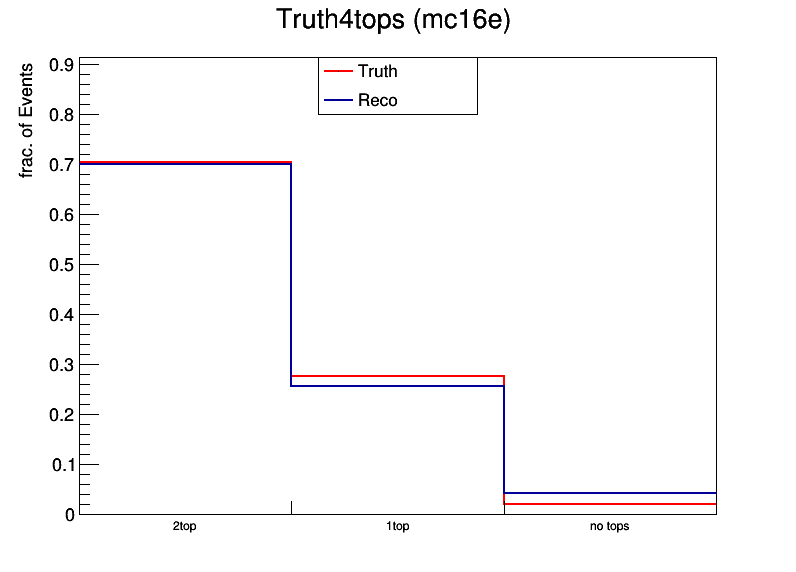
\includegraphics[width=.99\linewidth]{figs/HadTop/4topResult}
  \caption{$t\bar{t}t\bar{t}$ events}
  \label{fig:Reco4t}
\end{subfigure}%
\begin{subfigure}{.5\textwidth}
  \centering
  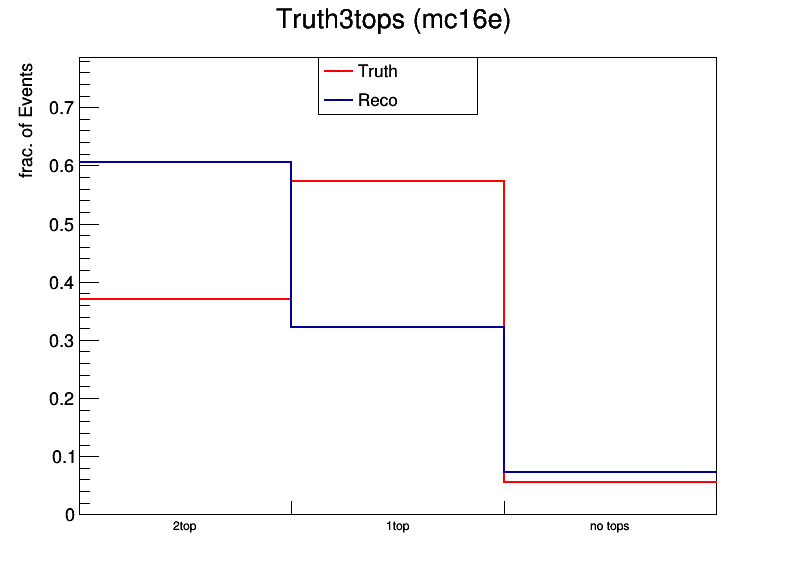
\includegraphics[width=.99\linewidth]{figs/HadTop/3topsResult}
  \caption{$t\bar{t}t$ events}
  \label{fig:Reco3t}
\end{subfigure}
\caption{Observed reconstruction where the critical values were tuned such that the fraction of events in all three channels fit the true $t\bar{t}t\bar{t}$ distribution.}
\label{fig:RecoResult}
\end{figure}

\vspace{-0.01cm}

Figure \ref{fig:RecoResult} shows the number of identified hadronic top quarks for the $t\bar{t}t\bar{t}$ and the $t\bar{t}t$ processes for the $\chi^2$ reconstruction (blue) and the true distribution (red). The critical values $\chi^2_{c1} = 5$ and $\chi^2_{c1} = 10$ are tuned such that the obtained results match the true $t\bar{t}t\bar{t}$ distribution. This results in a poor performance on the $t\bar{t}t$ dataset. In fact only 64\% of the events $t\bar{t}t\bar{t}$ and 43\% of the $t\bar{t}t$ events are categorized correctly to one or two hadronic top quark events. Most $t\bar{t}t$ one hadronic top quark events are reconstructed as two hadronic events and most non hadronic top quark events are reconstructed as one hadronic top quark events. The most likely explanation for this behavior is that the dominant production channel of $t\bar{t}t$ is associated production with a W boson. In fact, the original branching fraction of 0.72 is increased due to the signal region cuts to 0.99. In the case where the additional W boson decays hadronically, a hadronic top quark decay can be easily faked. The additional W boson is also the reason why at truth level not all $t\bar{t}t$ events in the signal region have one hadronic top quark. The signal region requirement of two same sign leptons can be achieved for a two hadronic $t\bar{t}t$ event when the additional W boson decays leptonically. \\
The poor performance (only 64\% of all events a categorized correctly) for the $t\bar{t}t\bar{t}$ is not apparent. The comparison of $\delta R(\text{reco},\text{truth})$ between the $\chi^2$ based reconstruction and the best-possible reconstruction, shown in Figure \ref{fig:dR}, shows that in most cases the incorrect jet combinations were selected. Furthermore, the kinematic distribution of the reconstructed objects differ in some cases from the truth and best-possible reconstruction distributions, shown in Figure \ref{fig:kinReco}. \\
A possible improvement of the $\chi^2$ based reconstruction can be the introduction of an additional term proportional to the MV2c10 scores for the jets assumed to be the b-jet of the top quark decay. Another way to improve the performance is to reconstruct the leptonically decaying W  bosons additionally. The difficulty in the reconstruction of multiple leptonically decaying W bosons is the allocation of $E_{T}^{miss}$ to multiple neutrinos, which was the reason why this approach was not considered for this study.

\newpage

\begin{figure}[H]
\begin{subfigure}{.5\textwidth}
  \centering
  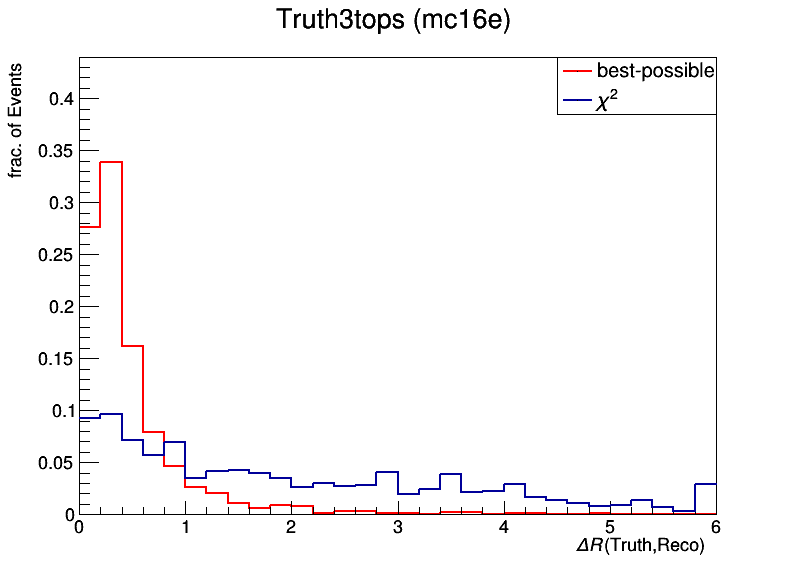
\includegraphics[width=.99\linewidth]{figs/HadTop/Chi3tops}
  \caption{}
  \label{fig:dR3}
\end{subfigure}%
\begin{subfigure}{.5\textwidth}
  \centering
  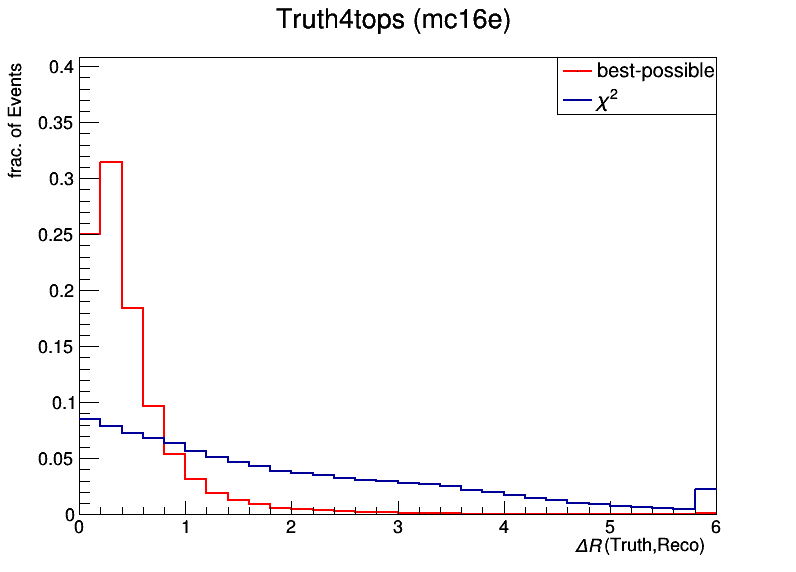
\includegraphics[width=.99\linewidth]{figs/HadTop/Chi4tops}
  \caption{}
  \label{fig:dR4}
\end{subfigure}
\caption{$\Delta R$ between the reconstructed top quarks and the truth top quarks for the $t\bar{t}t\bar{t}$ process (a) and the $t\bar{t}t$ process (b). The last bin contains additionally all reconstructed top quarks with $\Delta R > 6$.}
\label{fig:dR}
\end{figure}

\begin{figure}[H]
\begin{subfigure}{.5\textwidth}
  \centering
  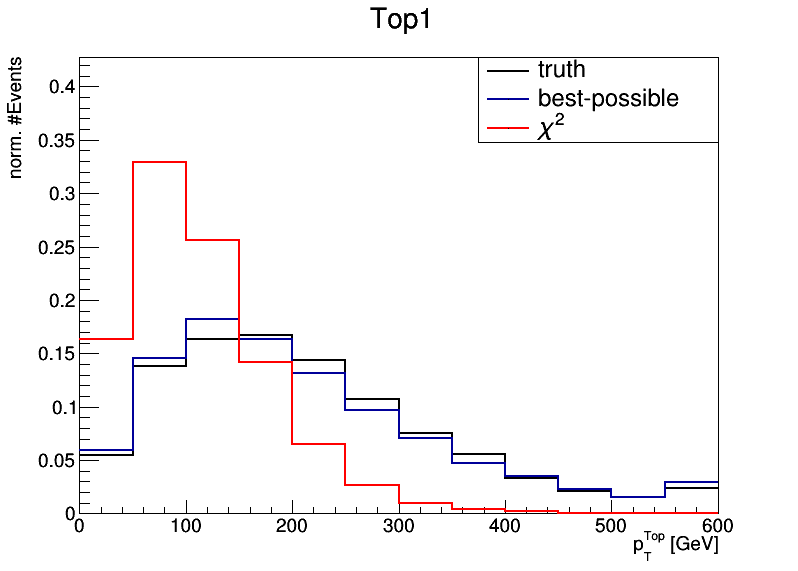
\includegraphics[width=.99\linewidth]{figs/HadTop/pt1hadtop1}
  \caption{Top $p_{\text{T}}$ for the one hadronic top category}
  \label{fig:pthad1}
\end{subfigure}%
\begin{subfigure}{.5\textwidth}
  \centering
  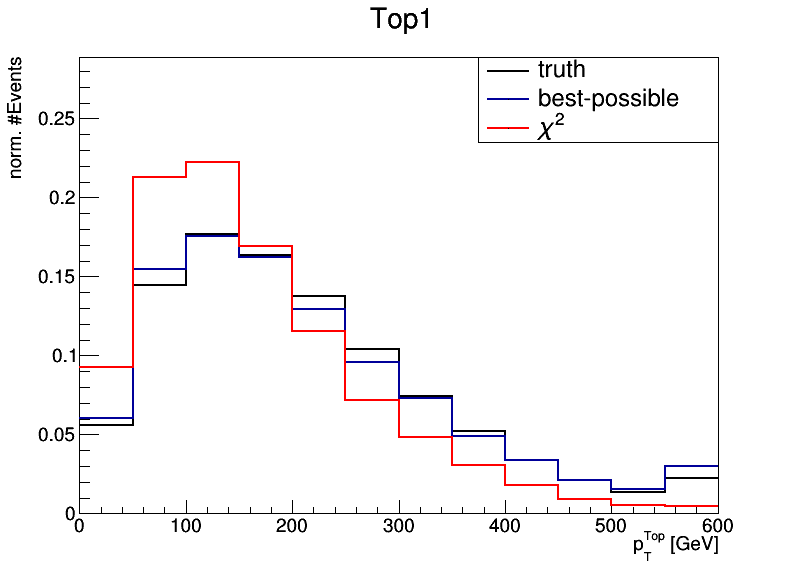
\includegraphics[width=.99\linewidth]{figs/HadTop/pt2hadtop1}
  \caption{Top $p_{\text{T}}$ for the two hadronic top category}
  \label{fig:pthad2}
\end{subfigure}
\begin{subfigure}{.5\textwidth}
  \centering
  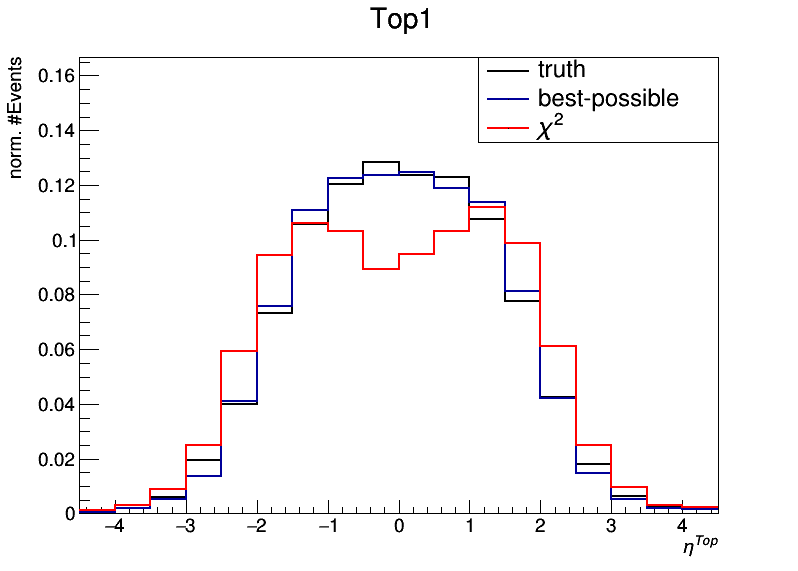
\includegraphics[width=.99\linewidth]{figs/HadTop/etatop}
  \caption{Top $\eta$ for the one hadronic top category}
  \label{fig:etat}
\end{subfigure}%
\begin{subfigure}{.5\textwidth}
  \centering
  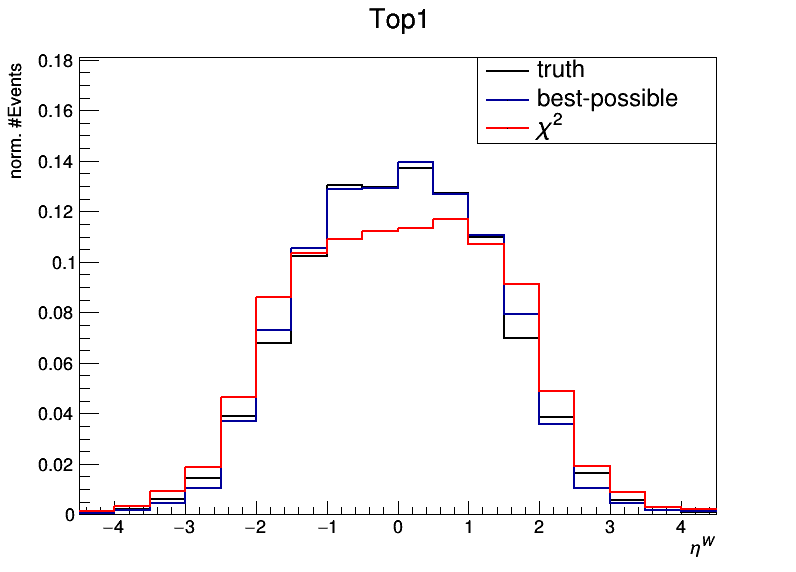
\includegraphics[width=.99\linewidth]{figs/HadTop/etaW}
  \caption{W boson $\eta$ for the one hadronic top category}
  \label{fig:etaW}
\end{subfigure}
\caption{Kinematic distributions for the truth and reconstructed top quarks and W bosons. The last bin in all distribution contains additionally the events which fall into bins above the maximum x-axis range.}
\label{fig:kinReco}
\end{figure}
